\documentclass[11pt]{amsart}
\usepackage[T1]{fontenc}
\usepackage[utf8]{inputenc}
\usepackage[english]{babel}
\usepackage{lmodern}
\usepackage{amsmath,amssymb,mathtools}
\usepackage{booktabs,array,longtable}
\usepackage{graphicx}
\usepackage{tikz}
\usetikzlibrary{arrows.meta,positioning,calc}
\usepackage{url}
\usepackage{enumitem}
\usepackage{float}
\usepackage{microtype}
\emergencystretch=2em
\usepackage[hidelinks]{hyperref}
\hypersetup{
  pdftitle={Proposal for a Descriptive Mechanism of the Asymptotic Wave: Observable Structural Compression through a Matrix Formalism},
  pdfauthor={Germán García Andrés},
  pdfsubject={Asymptotic wave; observable structural compression; matrix involutions; Riemann zeta and xi functions; prime-weighted states; passive-adjoint criteria},
  pdfkeywords={asymptotic wave, structural compression, matrix formalism, Riemann Hypothesis, xi function, critical reflection, nodal cancellation, commutation law, quaternionic lift, Smith coordinate, passive operators},
  pdfcreator={LaTeX / AMS article class},
  pdfproducer={pdfTeX},
  pdfinfo={DOI={10.5281/zenodo.22695552},RelatedDOI={10.5281/zenodo.22117063}}
}

\newtheorem{theorem}{Theorem}[section]
\newtheorem{proposition}[theorem]{Proposition}
\newtheorem{lemma}[theorem]{Lemma}
\newtheorem{corollary}[theorem]{Corollary}
\theoremstyle{definition}
\newtheorem{definition}[theorem]{Definition}
\newtheorem{algorithmicdef}[theorem]{Procedure}
\theoremstyle{remark}
\newtheorem{remark}[theorem]{Remark}
\newtheorem{scope}[theorem]{Scope condition}

\title[Asymptotic Wave and Matrix Compression]{Proposal for a Descriptive Mechanism of the Asymptotic Wave:\\ Observable Structural Compression through a Matrix Formalism}
\author{Germán García Andrés}
\thanks{Independent Researcher. Primary DOI: \href{https://doi.org/10.5281/zenodo.22695552}{10.5281/zenodo.22695552}. Related Spanish version DOI: \href{https://doi.org/10.5281/zenodo.22117063}{10.5281/zenodo.22117063}.}
\address{Independent Researcher}
\date{Final integrated revision with relativistic prime-wave extension, September 12, 2026}
\subjclass[2020]{11M26, 05C50, 55N31}
\keywords{asymptotic wave, observable structural compression, matrix formalism, Riemann Hypothesis, xi function, symmetry, involution, nodal cancellation, commutation law, quaternionic lift, Smith coordinate, prime angular field, Euler product, Fourier selector, arithmetic drum, relativistic prime wave, standing wave, sonification, passive operators}

\begin{document}
\begin{abstract}
We present an analytic--topological framework for studying the nontrivial zeros of the Riemann zeta function through involutions, orbits, induced operators, complementary graphs, and a dimensionless amplitude--phase state space.  Its central descriptive mechanism is the asymptotic mode $e^{(\beta-1/2)u}e^{i\gamma u}$ represented on the two scalar axes $x=\beta-1/2$ and $y=\gamma$.  The critical involution acts by the diagonal matrix $J_c=\operatorname{diag}(-1,1)$: it reverses the transverse coordinate and preserves the longitudinal coordinate.  The associated commuting projectors separate the observable fixed component from the confinement defect, while the distinct nodal involution $J_n=-I_2$ produces the rank-zero cancellation $I_2+J_n=O_2$.  This distinction prevents the null matrix, the identity, and the rank-one critical projection from being conflated.  The matrix law of commutation is linked to the graph identity $[L,P_R]=0$.  Occupied coordinate nodes are indexed losslessly on one discrete line by Cantor pairing, while a nested-cubical lemma states the exact condition under which transverse width collapses to zero.  Under the M\"obius coordinate $w(\rho)=1-1/\rho$, critical reflection preserves phase and inverts radial amplitude.  A paired quaternionic lift $Q_\rho=w(\rho)+w(R\rho)j$ combines the direct and reflected Smith coordinates, represents reflection by an exact component-exchange involution, and yields a nonnegative fixed-point defect.  The direct and reflected prime amplitudes similarly define two signed square-root branches; their squared separation yields a positive prime-channel defect, and summation over the analytic zero set gives an exact finite-height criterion for absence of the $F_4$ sector.  Buckingham reduction produces $K=(\beta-1/2)/\gamma$ and reciprocal cycle gains $e^{\pm2\pi K}$; bilateral passivity confines any independently realized reflected pair to $K=0$.  We integrate these statements with the $F_2/F_4$ orbit classification, prime-weighted coordinates, frozen out-of-sample tests, and the monopolar operator extension.  An Euler--Fourier arithmetic drum now supplies an exact prime--singularity bridge on $\Re s>1$: its heat trace is $\zeta(s)$, while its logarithmic derivative is a uniquely resolvable prime-power frequency comb $m\log p$.  A finite $10{,}001$-prime sonification and graphical audit preserve the declared frequencies, amplitudes, and phases.  A relativistic scaling $\kappa=c/L_0$ maps every arithmetic channel to $k_{p,m}=m\log(p)/L_0$ and $\omega_{p,m}=ck_{p,m}$; equal counterpropagating branches form an even standing wave with zero directional imbalance.  Exact identities, equivalent or conditional confinement criteria, and empirical results are kept logically separate; in particular, neither the acoustic nor relativistic reconstruction is substituted for the independent self-adjoint spectral realization required by the universal RH implication.
\end{abstract}
\maketitle
\begin{center}
\small\textbf{DOI:} \href{https://doi.org/10.5281/zenodo.22695552}{10.5281/zenodo.22695552}
\end{center}

\section{Object and scope}
The Riemann Hypothesis (RH) states that every nontrivial zero $\rho$ of $\zeta(s)$ satisfies
\begin{equation}\label{eq:RH}
   \Re(\rho)=\frac12.
\end{equation}
The official formulation of the Clay Mathematics Institute is precisely the universal statement \eqref{eq:RH}. The aim of this manuscript is to present, in reproducible detail, the method developed to: (i) express symmetry closure in terms of involutions and orbits; (ii) classify the orbits into $F_2$ and $F_4$ families; (iii) construct null, neutral, and non-null graphs; (iv) identify clusters through the Laplacian and $H_0$ persistence; (v) represent the symmetry by an operator $P_R$ and study its commutation with the Laplacian; (vi) organize a generational hierarchy; and (vii) formulate a strengthened criterion that, when certified globally, yields RH together with simplicity.

The mathematical core is complex-analytic, topological, spectral, matrix-theoretic, and dynamical.  The asymptotic-wave section gives the two-axis realization, its commuting involutions and projectors, and the exact distinction between transverse compression and total nodal cancellation.  In parallel, the monopole section develops a physical operator-theoretic extension based on the radial $L=0$ mode, while explicitly preserving the distinction between the nuclear operator and the graph-symmetry operator.  The revised extension also distinguishes three logically different assertions: an exact coordinate identity, a conditional confinement theorem, and a statistical predictor assessed on held-out data.  This separation is used throughout.

\section{Conceptual map and main results}\label{sec:mainresults}
The complete architecture can be read from left to right as
\begin{equation}\label{eq:roadmap}
\boxed{\begin{aligned}
\xi &\longrightarrow (C,F,R)\longrightarrow F_2/F_4\longrightarrow P_R,\\
P_R &\longrightarrow [L,P_R]=0\longrightarrow (J_c,J_n)\longrightarrow [J_c,J_n]=0,\\
(J_c,J_n)&\longrightarrow (P_{\parallel},P_{\perp},O_2)\longrightarrow B_n
\longrightarrow N(B_n)=1\longrightarrow \mathrm{RH}+\text{simplicity}.
\end{aligned}}
\end{equation}
Each arrow has a different role: the first ones describe analytic symmetry and its graphical representation; the intermediate ones introduce the spectral language; and the last one applies the argument principle to invariant regions.

\subsection{Results stated at the outset}
\begin{enumerate}[label=\textbf{R\arabic*.},leftmargin=*]
\item \textbf{Exact critical characterization.} For every nontrivial zero $\rho$,
\[
\Delta_R(\rho)=0\iff R(\rho)=\rho\iff F(\rho)=C(\rho)\iff \Re(\rho)=\frac12.
\]
The proof appears in Proposition~\ref{prop:residual}.
\item \textbf{Operator representation.} The assignment from zeros to vertices is equivariant,
\[
Q\circ R=P_R\circ Q,
\]
and, if $P_R$ preserves the graph edges, then $P_R^2=I$ and $[L,P_R]=0$; see Propositions~\ref{prop:equivariance} and~\ref{prop:lapcomm}.
\item \textbf{Global criterion.} RH is equivalent to every nontrivial zero belonging to the fixed sector of $R$, or equivalently to $\Delta_R(\rho)=0$ for every $\rho\in Z^*$.
\item \textbf{Extension to simplicity.} Theorem~\ref{thm:unitcells} establishes the equivalence between RH plus simplicity of all zeros and the existence, for every zero, of an $R$-invariant region with unit index $N(B_n)=1$.
\item \textbf{Coordinate-node and Cantor closure.}  The map
$\Phi(\rho)=(\Re\rho-1/2,\Im\rho)$ identifies every zero position with one occupied
coordinate node.  The two commuting reflections generate the four-node Klein orbit and its
null average; symmetry plus unit-cell uniqueness, rather than the null average alone, forces
the fixed node.  Cantor pairing then gives a reversible one-dimensional address for every
occupied cell.  Nested cubical slabs with transverse widths tending to zero provide an exact
intersection criterion for $\Re\rho=1/2$.
\item \textbf{Closure by set saturation.} For each finite height $T$, an inclusion $S(T)\subseteq Z_2(T)\subseteq Z^*(T)$ together with the counting equality $|S(T)|=N(T)=\sum_{\rho\in Z^*(T)}m(\rho)$ forces $S(T)=Z_2(T)=Z^*(T)$; hence $Z_4(T)=\varnothing$. An exhaustive sequence $T_k\to\infty$ transfers the closure to the entire critical strip.
\item \textbf{Dimensionless reflected dynamics.} For $\rho=\beta+i\gamma$, $\gamma\ne0$, the Buckingham parameter
\[
K_\rho=\frac{\beta-1/2}{\gamma}
\]
controls radial gain per unit phase.  The critical reflection sends $K_\rho$ to $-K_\rho$, so the two cycle gains are reciprocal.  If both reflected branches are realized in a common forward-passive architecture, they must have unit gain and hence $K_\rho=0$.
\item \textbf{Predictive state extension.} The unfolded ordinate, two quadrature coordinates, and a normalized prime-angular field define a four-dimensional state.  A frozen localizer is evaluated on held-out transitions and compared with the neutral predictor; the resulting scores are empirical ranking quantities, not probabilities of an exact zero on a continuum.
\item \textbf{Two-axis matrix compression and commutation.}  With
$x=\Re\rho-1/2$ and $y=\Im\rho$, the critical involution is
$J_c=\operatorname{diag}(-1,1)$ and the nodal involution is $J_n=-I_2$.
They commute, their projectors isolate the $x$ and $y$ axes, and
$I_2+J_n=O_2$ gives the exact rank-zero cancellation.  Critical confinement,
by contrast, is the rank-one condition $P_{\perp}\mathbf a=0$, which is
equivalent to $x=0$.
\item \textbf{Signed square-root prime defect.}  For finite nonempty prime-power
cutoffs, the weighted squared separation of the reciprocal reflected amplitudes is
nonnegative and even in $a=\Re\rho-1/2$.  Its two square-root branches are $\pm$,
the corresponding oriented defect is odd under reflection, and the two branches meet
only at $a=0$.  Summing the squared defect over $Z^*(T)$ with multiplicity vanishes
exactly when $Z_4(T)$ is empty.
\item \textbf{Prime--singularity bridge and universal-route reduction.}  The diagonal
Euler Hamiltonian has partition trace $\zeta(s)$ for $\Re s>1$.  Logarithmic
differentiation produces the discrete prime-power frequency comb $m\log p$, and
long-time Fourier averaging extracts every coefficient uniquely.  A reproducible
$10{,}001$-prime sonification and four-panel graphical audit realize the finite
arithmetic identities.  The same construction yields the exact reduction
$E_\rho\in\mathbb R\iff\Re\rho=1/2$ and states, as one fixed target rather than an
open-ended list, the independent spectral realization that turns this equivalence into RH.
\item \textbf{Relativistic prime-wave realization.}  Introducing one reference length
$L_0$ fixes the dimensional scale $\kappa=c/L_0$.  The arithmetic Hamiltonian becomes
$\mathsf H_{\rm pr}=(\hbar c/L_0)H_E$, each channel obeys the massless dispersion
$\omega_{p,m}=ck_{p,m}$, and equal counterpropagating components generate an even standing
wave.  The arithmetic angular-momentum operators commute with $\mathsf H_{\rm pr}$, while
the passive term has an explicit nonpositive norm derivative.  A reproducible finite-difference
audit verifies second-order convergence of the wave-equation residual.
\end{enumerate}

\subsection{Status of the statements}
For clarity, five levels of content are distinguished:
\begin{center}
\begin{tabular}{p{0.25\linewidth}p{0.66\linewidth}}
\toprule
\textbf{Level} & \textbf{Content}\\
\midrule
Exact result & Symmetry identities, characterization of $\operatorname{Fix}(R)$, $F_2/F_4$ classification, equivariance, and commutation under a graph automorphism.\\
Derived theorem & Strengthened unit-cell criterion and its equivalence with RH plus simplicity.\\
Computational result & Null--neutral--non-null graphs, Laplacian spectra, and $H_0$ persistence on finite blocks of ordinates.\\
Operator extension & Nuclear $L=0$ monopole operator, collective Hamiltonian, and architectural comparison with the graph operator.\\
State extension & Exact Buckingham and reflection identities; conditional bilateral-passivity confinement; and separately labelled out-of-sample numerical localization.\\
Matrix extension & Exact two-axis involutions, commuting projectors, null/identity distinction, and a commutation criterion linking the scalar, matrix, and graph representations.\\
Set-theoretic extension & Exact node intersection, Klein-orbit averaging, Cantor indexing, and nested-cubical confinement implications, with their non-circularity conditions stated explicitly.\\
Acoustic arithmetic extension & Exact Euler trace, prime-power Fourier comb, coefficient selector, finite diagonal drum, $10{,}001$-prime sonification, and an explicitly conditional spectral-reality closure.\\
Relativistic wave extension & Dimensionally consistent $c/L_0$ scaling, massless dispersion, standing-wave superposition, conserved arithmetic angular momentum, passive norm balance, and a numerical PDE audit.\\
\bottomrule
\end{tabular}
\end{center}

\subsection{Minimal table of symbols}
\begin{center}
\begin{tabular}{p{0.18\linewidth}p{0.72\linewidth}}
\toprule
\textbf{Symbol} & \textbf{Meaning}\\
\midrule
$C(s)$ & Complex conjugation $\overline{s}$.\\
$F(s)$ & Functional reflection $1-s$.\\
$R(s)$ & Critical involution $1-\overline{s}$.\\
$\Delta_R$ & Closure residual $F(\rho)-C(\rho)=1-2\Re(\rho)$.\\
$F_2,F_4$ & Critical and generic geometric orbits, respectively.\\
$Q$ & Assignment of a zero to its vertex; in the generational layer a scalar quotient is also denoted by $Q$, explicitly indicated by context.\\
$P_R$ & Permutation operator induced by $R$ on the vertices.\\
$A,D,L$ & Adjacency, degree, and Laplacian matrices, $L=D-A$.\\
$\beta_0$ & Number of connected components, $\dim\ker L$.\\
$B_n$ & $R$-invariant Jordan region associated with the zero $\rho_n$.\\
$N(B)$ & Number of zeros of $\xi$ in $B$, counted with multiplicity.\\
$\mathcal J$ & Radial involution $x\mapsto -x$ in the monopole extension.\\
$\widehat H_M$ & Quantized collective Hamiltonian of the ideal monopole mode.\\
$K_\rho$ & Dimensionless radial-to-angular rate $(\Re\rho-1/2)/\Im\rho$.\\
$x,y$ & Scalar transverse and longitudinal coordinates, $x=\Re\rho-1/2$ and $y=\Im\rho$.\\
$J_c,J_n$ & Critical reflection $\operatorname{diag}(-1,1)$ and nodal inversion $-I_2$.\\
$P_{\parallel},P_{\perp}$ & Commuting projectors onto the preserved $y$ axis and transverse $x$ axis.\\
$O_2,I_2$ & Rank-zero null matrix and multiplicative identity; they are distinct neutral objects.\\
$\mathfrak n_\rho$ & Occupied coordinate node $\{(\Re\rho-1/2,\Im\rho)\}$.\\
$\eta,\pi,\kappa$ & Signed-integer code, Cantor pairing function, and one-dimensional occupied-node index.\\
$\mathcal C_n$ & Nested cubical slab with transverse half-width $\varepsilon_n\downarrow0$.\\
$Q_\Lambda(\gamma)$ & Normalized prime-angular coordinate in $[0,1]$.\\
$\mathbf S_n^{(d)}$ & State attached to the $n$th ordinate in $d$ coordinates.\\
\bottomrule
\end{tabular}
\end{center}

\section{Established analytic preliminaries}
\subsection{Zeta, trivial zeros, and the completed function}
The function $\zeta(s)$, initially defined for $\Re(s)>1$ by
\begin{equation}
  \zeta(s)=\sum_{n=1}^{\infty}n^{-s},
\end{equation}
extends meromorphically to the complex plane with a simple pole at $s=1$. The functional equation implies the trivial zeros
\begin{equation}
  -2,-4,-6,\ldots.
\end{equation}
All remaining zeros lie in the critical strip $0<\Re(s)<1$ and are called nontrivial zeros.

It is useful to work with Riemann's entire xi function
\begin{equation}\label{eq:xi}
 \xi(s)=\frac12 s(s-1)\pi^{-s/2}\Gamma\!\left(\frac{s}{2}\right)\zeta(s),
\end{equation}
which satisfies
\begin{equation}\label{eq:functionalxi}
   \xi(s)=\xi(1-s)
\end{equation}
and whose zeros are exactly the nontrivial zeros of $\zeta$, counted with multiplicity.

\subsection{Conjugation and reflection}
We define
\begin{equation}\label{eq:CFR}
  C(s)=\overline{s},\qquad F(s)=1-s,\qquad R(s)=F(C(s))=1-\overline{s}.
\end{equation}
All three transformations are involutions:
\begin{equation}
 C^2=F^2=R^2=I.
\end{equation}
Moreover, the reality of the coefficients together with \eqref{eq:functionalxi} implies that these transformations preserve the zero set of $\xi$.

\section{Symmetry families: $F_2$ and $F_4$}
Let
\begin{equation}
 \rho=\sigma+i\gamma
\end{equation}
be a nontrivial zero. Consider the orbit under the transformations generated by $C$ and $F$:
\begin{equation}\label{eq:orbit}
 \mathcal O(\rho)=\{\rho,\overline\rho,1-\rho,1-\overline\rho\}.
\end{equation}

\begin{definition}[$F_4$ family]
If $\sigma\neq1/2$ and $\gamma\neq0$, the four elements of \eqref{eq:orbit} are generically distinct. We denote this orbit by $F_4$.
\end{definition}

\begin{definition}[$F_2$ family]
If $\sigma=1/2$, then
\begin{equation}\label{eq:F2collapse}
  1-\rho=\overline\rho,\qquad 1-\overline\rho=\rho,
\end{equation}
and the orbit reduces to two geometric positions:
\begin{equation}
 F_2(\gamma)=\left\{\frac12+i\gamma,\frac12-i\gamma\right\}.
\end{equation}
\end{definition}

\begin{proposition}[Reversible-closure residual]\label{prop:residual}
Define
\begin{equation}\label{eq:delta}
 \Delta_R(\rho)=F(\rho)-C(\rho).
\end{equation}
Then
\begin{equation}\label{eq:deltaeval}
 \Delta_R(\rho)=1-2\Re(\rho),
\end{equation}
and therefore
\begin{equation}\label{eq:equiv}
 \Delta_R(\rho)=0
 \iff F(\rho)=C(\rho)
 \iff R(\rho)=\rho
 \iff \Re(\rho)=\frac12.
\end{equation}
\end{proposition}

\begin{proof}
For $\rho=\sigma+i\gamma$,
\[
F(\rho)-C(\rho)=1-\sigma-i\gamma-(\sigma-i\gamma)=1-2\sigma.
\]
Thus $\Delta_R=0$ if and only if $\sigma=1/2$. Moreover, $R(\rho)=\rho$ is equivalent to $1-\overline\rho=\rho$, which yields the same real equality $1-\sigma=\sigma$.
\end{proof}

\begin{corollary}[Fixed set]
\begin{equation}
 \operatorname{Fix}(R)=\{s\in\mathbb C:\Re(s)=1/2\}.
\end{equation}
In particular, RH is equivalent to all nontrivial zeros belonging to $\operatorname{Fix}(R)$.
\end{corollary}

\subsection{Minimal worked example: critical closure versus generic orbit}\label{sec:workedexample}
To visualize the classification without depending on a numerical table of zeros, first consider the critical model point
\[
\rho_c=\frac12+14i.
\]
Then
\[
C(\rho_c)=\frac12-14i,\qquad F(\rho_c)=\frac12-14i,\qquad R(\rho_c)=\rho_c,
\]
and
\[
\Delta_R(\rho_c)=0,
\qquad
\mathcal O(\rho_c)=\left\{\frac12+14i,\frac12-14i\right\}.
\]
By construction, the model belongs to the $F_2$ pattern: the $C$ and $F$ routes have the same image and $R$ fixes the point.

As a logical contrast, consider the off-line point
\[
\rho_o=0.4+14i.
\]
One obtains
\[
C(\rho_o)=0.4-14i,\qquad F(\rho_o)=0.6-14i,\qquad R(\rho_o)=0.6+14i,
\]
\[
\Delta_R(\rho_o)=0.2\neq0,
\]
and the orbit contains four distinct positions,
\[
\mathcal O(\rho_o)=\{0.4\pm14i,\;0.6\pm14i\}.
\]
This second point is a geometric counterexample to $F_2$ closure, not a claim that it is a zero of $\zeta$. The pair of examples shows exactly what the identifier detects before the graph is introduced: equality of images in the critical case and transverse duplication in the generic case.

\section{Symmetry graph for identifying the families}
The first graph does not use numerical proximity; it encodes exactly the action of the involutions.

\begin{definition}[Symmetry graph $\mathcal G_{\rm sym}(\rho)$]
The vertices are the distinct elements of $\mathcal O(\rho)$. Edges labelled by $C$, $F$, and $R$ are added between a vertex $z$ and its image under each transformation. The labels are retained even when two transformations have the same image.
\end{definition}

For a generic $F_4$ orbit, with
\[
v_1=\rho,\quad v_2=\overline\rho,\quad v_3=1-\rho,\quad v_4=1-\overline\rho,
\]
the edges are
\begin{align*}
C:&\ (v_1,v_2),(v_3,v_4),\\
F:&\ (v_1,v_3),(v_2,v_4),\\
R:&\ (v_1,v_4),(v_2,v_3).
\end{align*}
After forgetting the labels, the underlying graph is $K_4$, with
\begin{equation}
A_{F_4}=\begin{pmatrix}
0&1&1&1\\1&0&1&1\\1&1&0&1\\1&1&1&0
\end{pmatrix},\qquad
L_{F_4}=3I-A_{F_4},
\end{equation}
and spectrum
\begin{equation}
 \operatorname{Spec}(L_{F_4})=\{0,4,4,4\}.
\end{equation}

In $F_2$, the identifications in \eqref{eq:F2collapse} produce two vertices. The labels $C$ and $F$ describe the same transposition, while $R$ fixes each vertex. The simple quotient graph is $K_2$:
\begin{equation}
A_{F_2}=\begin{pmatrix}0&1\\1&0\end{pmatrix},\qquad
L_{F_2}=\begin{pmatrix}1&-1\\-1&1\end{pmatrix},
\end{equation}
with
\begin{equation}
 \operatorname{Spec}(L_{F_2})=\{0,2\}.
\end{equation}
Thus the orbit size and the quotient graph distinguish exactly the critical case from the generic one. This classification supplies the algebraic identifier used later in the global cell criterion.

\begin{figure}[t]
\centering
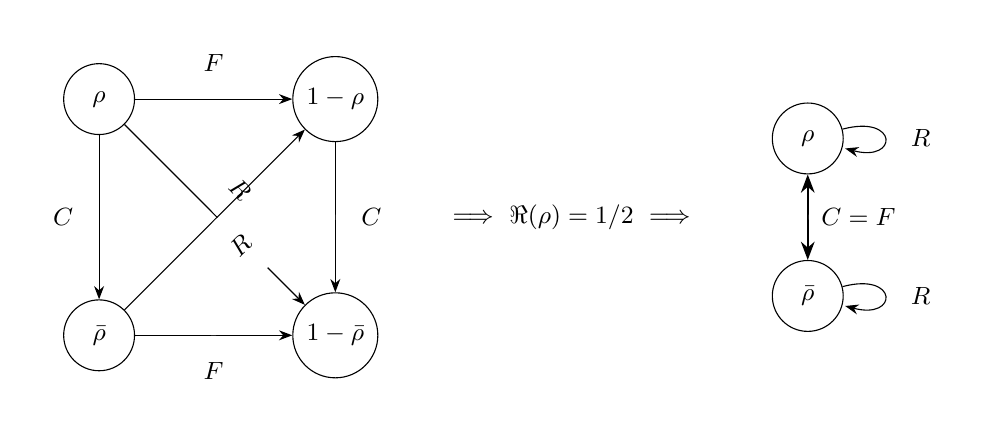
\begin{tikzpicture}[>=Stealth, every node/.style={circle,draw,minimum size=9mm,font=\small}]
\node (a) at (0,1.5) {$\rho$};
\node (b) at (0,-1.5) {$\bar\rho$};
\node (c) at (3,1.5) {$1-\rho$};
\node (d) at (3,-1.5) {$1-\bar\rho$};
\draw[->] (a) -- node[left,draw=none,fill=white] {$C$} (b);
\draw[->] (a) -- node[above,draw=none,fill=white] {$F$} (c);
\draw[->] (a) -- node[sloped,above,draw=none,fill=white] {$R$} (d);
\draw[->] (c) -- node[right,draw=none,fill=white] {$C$} (d);
\draw[->] (b) -- node[below,draw=none,fill=white] {$F$} (d);
\draw[->] (b) -- node[sloped,below,draw=none,fill=white] {$R$} (c);
\node[draw=none] at (6,0) {$\Longrightarrow\ \Re(\rho)=1/2\ \Longrightarrow$};
\node (e) at (9,1) {$\rho$};
\node (f) at (9,-1) {$\bar\rho$};
\draw[<->,thick] (e) -- node[right,draw=none,fill=white] {$C=F$} (f);
\path[->] (e) edge[loop right] node[right,draw=none] {$R$} (e);
\path[->] (f) edge[loop right] node[right,draw=none] {$R$} (f);
\end{tikzpicture}
\caption{Labelled graph of the generic $F_4$ orbit and its geometric collapse to $F_2$ when $1-\rho=\bar\rho$. The labels represent distinct transformations even when they coincide in their image.}
\label{fig:symgraph}
\end{figure}

\section{Induced operator and commutation of the two languages}
Let $Z^*$ denote the set of nontrivial zeros and let
\[
Q:Z^*\longrightarrow V(\mathcal G_{\rm sym}),\qquad Q(\rho)=v_{\rho},
\]
be the assignment of each zero to its vertex. The involution $R(s)=1-\overline{s}$ induces a linear permutation of the vertices,
\begin{equation}\label{eq:PR}
P_R v_{\rho}=v_{R(\rho)}.
\end{equation}
Since $R^2=I$, one also has
\begin{equation}
P_R^2=I,\qquad P_R^{-1}=P_R.
\end{equation}

\begin{proposition}[Equivariance of the identifier]\label{prop:equivariance}
The assignment $Q$ between zeros and vertices is equivariant with respect to $R$ and $P_R$:
\begin{equation}\label{eq:commdiagram}
Q\circ R=P_R\circ Q.
\end{equation}
In particular,
\[
Q(\operatorname{Fix}R)=\operatorname{Fix}(P_R)\cap Q(Z^*).
\]
\end{proposition}

\begin{proof}
By definition, $(Q\circ R)(\rho)=Q(R(\rho))=v_{R(\rho)}$, whereas $(P_R\circ Q)(\rho)=P_Rv_{\rho}=v_{R(\rho)}$. The equality of fixed sets follows immediately.
\end{proof}

\begin{proposition}[Commutation with the Laplacian]\label{prop:lapcomm}
If the action of $P_R$ preserves the edges of the graph under consideration, then $P_R$ is an automorphism and
\begin{equation}\label{eq:lapcomm}
P_RAP_R^{-1}=A,\qquad P_RDP_R^{-1}=D,
\end{equation}
so that
\begin{equation}
P_RLP_R^{-1}=L,\qquad [L,P_R]=0,
\end{equation}
with $L=D-A$.
\end{proposition}

\begin{proof}
An automorphism preserves adjacency and degrees. The two identities in \eqref{eq:lapcomm} follow from the permutation-matrix representation; subtracting them yields invariance of $L$. Since $P_R^{-1}=P_R$, invariance is equivalent to $LP_R=P_RL$.
\end{proof}

The preceding commutation has two precise interpretations. In $\mathcal G_{\rm sym}$ it is an exact consequence of the symmetry action used to construct the orbit. In graphs obtained from an independent rule, the equality $[L,P_R]=0$ is a structural test that the resulting architecture preserves the same involution. In this way, the complex symmetry and the spectral language of the graph are linked by the commutative diagram \eqref{eq:commdiagram}.

\section{Generations: from primary families to secondary zeta functions}
The term \emph{generation} is used here with an explicit distinction between established literature and the proposed extension.

\subsection{First generation: families of zeros}
The first generation consists of the orbits of the nontrivial zeros under $C$ and $F$. On the critical line, each geometric family is
\begin{equation}
  F_2(\gamma_k)=\left\{\frac12+i\gamma_k,\frac12-i\gamma_k\right\}.
\end{equation}
When $\gamma_k>0$, quotienting by conjugation permits the scalar code
\begin{equation}\label{eq:Q}
 Q(F_2(\gamma_k))=\gamma_k^2.
\end{equation}
On its image, \eqref{eq:Q} is bijective, with inverse
\begin{equation}
 Q^{-1}(u)=\left\{\frac12+i\sqrt u,\frac12-i\sqrt u\right\},\qquad u>0.
\end{equation}

\subsection{Second generation: zeta functions built over zeros}
Voros studied zeta functions defined by Dirichlet series over the Riemann zeros. A fundamental form is
\begin{equation}\label{eq:superzeta}
 \mathcal Z(\sigma,v)=\sum_{k=1}^{\infty}(\tau_k^2+v)^{-\sigma},
\end{equation}
with meromorphic continuation in $\sigma$. In later literature these constructions are explicitly described as \emph{second-generation} zeta functions or \emph{superzeta functions}.

The literature allows two facts to be separated. Voros constructs second-generation zeta functions from the zeros, whereas Arias de Reyna formulates a secondary zeta function without presupposing RH, using parameters $\alpha_n$ defined by $\rho_n=1/2+i\alpha_n$. In the $F_2$ stratum, $\alpha_n=\gamma_n\in\mathbb R$ and the code $\gamma_k^2$ is real, one-dimensional, and reversible on the critical family; outside that stratum, the parameter may retain complex transverse information. This distinction fixes precisely the generational content used in the method.

\subsection{Proposed third layer: persistent topological families}
We propose organizing the positive codes $\gamma_k$, or their unfolded coordinates, by means of a proximity filtration. This third layer is not standard terminology in analytic number theory; it is a topological classification tool for studying whether similar clusters recur in blocks of zeros at different heights.

\section{Three control architectures: null, neutral, and non-null}
To separate structural zero eigenvalues that arise from the architecture itself from patterns specific to the Riemann ordinates, three controls with the same number $N$ of vertices are used.

\subsection{Null graph $\mathcal G_{\varnothing}$}
\begin{equation}
 E_{\varnothing}=\varnothing,\qquad A_{\varnothing}=0,\qquad L_{\varnothing}=0.
\end{equation}
Therefore,
\begin{equation}
 \operatorname{Spec}(L_{\varnothing})=\{0,\ldots,0\},\qquad \beta_0=N.
\end{equation}
This control represents the complete absence of connections.

\subsection{Neutral graph $\mathcal G_{\rm neu}(\varepsilon)$}
Equally spaced points are used,
\begin{equation}
 y_n=n,\qquad n=1,\ldots,N,
\end{equation}
with the same proximity rule that will be applied to the data:
\begin{equation}\label{eq:neutraledge}
 (i,j)\in E_{\rm neu}(\varepsilon)
 \iff |y_i-y_j|\le\varepsilon.
\end{equation}
Thus the neutral control has a single separation scale. For $\varepsilon=1$, the 1-skeleton is a connected path; component merging occurs essentially at a single scale.

\subsection{Non-null Riemann graph $\mathcal G_R(\varepsilon)$}
Each vertex corresponds to a positive ordinate $\gamma_n$ of a known zero on the critical line. Because the density changes with height, the ordinates are first unfolded using the smooth part of the Riemann--von Mangoldt formula:
\begin{equation}\label{eq:unfold}
 x_n=\overline N(\gamma_n),\qquad
 \overline N(T)=\frac{T}{2\pi}\log\frac{T}{2\pi}-\frac{T}{2\pi}+\frac78.
\end{equation}
An edge is activated by the same Rips rule:
\begin{equation}\label{eq:riemannedge}
 (i,j)\in E_R(\varepsilon)
 \iff |x_i-x_j|\le\varepsilon.
\end{equation}
We define
\begin{equation}
 A_R(\varepsilon)=(a_{ij}),\quad
 a_{ij}=\mathbf 1\{0<|x_i-x_j|\le\varepsilon\},
\end{equation}
\begin{equation}
 D_R(\varepsilon)=\operatorname{diag}(d_1,\ldots,d_N),\qquad
 L_R(\varepsilon)=D_R(\varepsilon)-A_R(\varepsilon).
\end{equation}
The multiplicity of the zero eigenvalue of the Laplacian equals the number of connected components:
\begin{equation}\label{eq:beta0}
 \beta_0(\varepsilon)=\dim\ker L_R(\varepsilon).
\end{equation}
As $\varepsilon$ varies, edges are activated monotonically, producing a Vietoris--Rips filtration. In dimension zero, every death of a persistence bar corresponds to a merger of components.

\section{Complete method, step by step}
\begin{algorithmicdef}[Reproducible pipeline]
The procedure used to identify families and clusters is as follows.
\begin{enumerate}[label=\textbf{Step \arabic*.},leftmargin=*]
\item \textbf{Analytic input.} Fix the transformations $C,F,R$ from \eqref{eq:CFR} and the orbit \eqref{eq:orbit}.
\item \textbf{Symmetry-family identification.} Construct $\mathcal G_{\rm sym}(\rho)$ and count distinct positions. If $R(\rho)=\rho$, the family is $F_2$; otherwise the generic orbit is $F_4$.
\item \textbf{Algebraic check.} Evaluate $\Delta_R=1-2\Re(\rho)$. Exact zero is equivalent to the critical line.
\item \textbf{Data selection.} Take an ordered block $\gamma_1<\cdots<\gamma_N$ of ordinates of verified zeros. Odlyzko's tables provide, for example, the first $100\,000$ zeros to high precision.
\item \textbf{Unfolding.} Transform $\gamma_n\mapsto x_n$ using \eqref{eq:unfold} to remove the smooth change in density.
\item \textbf{Null control.} Construct $\mathcal G_{\varnothing}$ with the same $N$ vertices and no edges.
\item \textbf{Neutral control.} Construct $\mathcal G_{\rm neu}(\varepsilon)$ on equally spaced points and use exactly the same values of $\varepsilon$.
\item \textbf{Non-null graph.} Construct $\mathcal G_R(\varepsilon)$ using the rule \eqref{eq:riemannedge}.
\item \textbf{Laplacian.} Compute $L=D-A$, its spectrum, and the multiplicity of $\lambda=0$ for each architecture.
\item \textbf{Filtration.} Sweep $\varepsilon$ without selecting an a posteriori threshold. Record the complete curve $\beta_0(\varepsilon)$ and the $H_0$ death times.
\item \textbf{Topological families.} Define a cluster at a given scale as a connected component of the Rips graph. The most persistent families are those separated by the largest death times; they are not selected manually.
\item \textbf{Comparison of architectures.} Contrast
\[
\mathcal B_{\varnothing}(\varepsilon),\quad
\mathcal B_{\rm neu}(\varepsilon),\quad
\mathcal B_R(\varepsilon),
\]
where $\mathcal B=\beta_0$.
\item \textbf{Statistical-topological self-similarity test.} Repeat the pipeline on disjoint blocks of zeros; compare the normalized curves $\beta_0(\varepsilon)/N$ and the persistence distributions. Stable agreement among blocks would constitute evidence of statistical topological universality, not by itself a proof of RH.
\item \textbf{Generational layer.} For $F_2$ families, apply the quotient $Q$ and, where appropriate, construct secondary objects of the form \eqref{eq:superzeta}. Keep this analytic generation separate from the topological classification by proximity.
\end{enumerate}
\end{algorithmicdef}

\section{Reproducible illustration with the first 300 zeros}
As a numerical control, the first $300$ positive zeros were computed with standard multiprecision arithmetic and the scale was checked against Odlyzko's public tables. After the unfolding \eqref{eq:unfold}, the $299$ consecutive gaps give
\begin{equation}
 \overline d=0.9985241,\qquad
 \operatorname{median}(d)=0.9591051,
\end{equation}
\begin{equation}
 d_{\min}=0.2910884,\qquad d_{\max}=1.9934329.
\end{equation}
Table \ref{tab:beta} shows the $H_0$ curve at eight predefined scales.

\begin{table}[t]
\centering
\caption{Number of components $\beta_0$ for $N=300$ at the same scale $\varepsilon$. The null graph activates no edges; the equally spaced neutral graph merges at the unit scale; the non-null Riemann graph exhibits a multiscale transition.}
\label{tab:beta}
\begin{tabular}{rrrr}
\toprule
$\varepsilon$ & $\beta_0(\mathcal G_{\varnothing})$ & $\beta_0(\mathcal G_{\rm neu})$ & $\beta_0(\mathcal G_R)$\\
\midrule
0.25 & 300 & 300 & 300\\
0.50 & 300 & 300 & 282\\
0.75 & 300 & 300 & 211\\
1.00 & 300 & 1   & 131\\
1.25 & 300 & 1   & 74\\
1.50 & 300 & 1   & 31\\
1.75 & 300 & 1   & 12\\
2.00 & 300 & 1   & 1\\
\bottomrule
\end{tabular}
\end{table}

At $\varepsilon=1.50$, there are $31$ components; the six largest component sizes are
\[
19,\;17,\;16,\;15,\;14,\;12.
\]
At $\varepsilon=1.75$, $12$ components remain; the six largest sizes are
\[
40,\;33,\;32,\;31,\;30,\;26.
\]
These groups are outputs of the $H_0$ filtration and must not be confused with the algebraic $F_2/F_4$ orbits.

Spectrally, at $\varepsilon=1$ the Riemann graph has $169$ edges and $131$ components, whereas the neutral control has $299$ edges and is connected. At $\varepsilon=2$ the Riemann graph is connected, with $448$ edges and mean degree $2.9867$. These values serve as implementation checks for the architecture, not as a truth criterion for RH.

\section{Laplacian zeros versus zeros of $\zeta$}
It is essential to keep two uses of the word \emph{zero} separate.

\begin{enumerate}[label=(\alph*)]
\item A zero of $\zeta$ or $\xi$ is a complex point $\rho$ such that $\xi(\rho)=0$.
\item A zero of the Laplacian is an eigenvalue $\lambda=0$ of $L$; its multiplicity is $\beta_0$, the number of connected components.
\end{enumerate}

The graph does not ``produce'' Riemann zeros. It uses previously computed zeros as vertices and produces topological invariants of their organization. By contrast, the symmetry graph $\mathcal G_{\rm sym}$ encodes exactly how each zero is related to its images under the functional equation and conjugation.

\section{Poles, inverses, and multiplicity}
The function $\zeta$ has a simple pole at $s=1$, whereas $\xi$ is entire. Nevertheless, the zeros of $\xi$ appear as poles of $1/\xi$ and of the logarithmic derivative $\xi'/\xi$.

If $\rho$ is a zero of multiplicity $m$, locally
\begin{equation}
 \xi(s)=(s-\rho)^m g(s),\qquad g(\rho)\neq0,
\end{equation}
and hence
\begin{equation}\label{eq:logder}
 \frac{\xi'(s)}{\xi(s)}=\frac{m}{s-\rho}+\frac{g'(s)}{g(s)}.
\end{equation}
Thus $\xi'/\xi$ has a simple pole at $\rho$ with residue $m$.

\begin{proposition}[Argument principle and extension to simplicity]
Let $B$ be a region whose boundary contains no zeros of $\xi$. Then
\begin{equation}
 N(B)=\frac{1}{2\pi i}\oint_{\partial B}\frac{\xi'(s)}{\xi(s)}\,ds
\end{equation}
counts zeros with multiplicity. If, in addition, $R(B)=B$ and $N(B)=1$, the unique zero in $B$ lies on $\Re(s)=1/2$ and is simple.
\end{proposition}

\begin{proof}
If $\rho\in B$ is a zero, then $R(\rho)$ is also a zero and belongs to $B$. Since $N(B)=1$, there can be neither two distinct positions nor multiplicity greater than one; therefore $R(\rho)=\rho$ and $m=1$. Proposition \ref{prop:residual} gives $\Re(\rho)=1/2$.
\end{proof}

\begin{remark}
The condition $N(B)=1$ contains two conclusions simultaneously: it fixes a unique geometric position inside an $R$-invariant region and fixes multiplicity one. Hence a global certification of unit cells yields a strictly strengthened conclusion: critical-line localization and simplicity.
\end{remark}

\section{Conditional global certification criterion}\label{sec:globalmechanism}
The logical route connecting the graph architecture to the strengthened result is summarized by
\begin{equation}\label{eq:globalchain}
\boxed{\begin{aligned}
\mathcal G &\Longrightarrow \{B_n\}_{n\ge1}
\Longrightarrow \bigl(R(B_n)=B_n,\;N(B_n)=1\bigr),\\
&\Longrightarrow R(\rho_n)=\rho_n
\Longrightarrow \Re(\rho_n)=\frac12,\;m(\rho_n)=1.
\end{aligned}}
\end{equation}
The content of each step is as follows.
\begin{enumerate}[label=\textbf{G\arabic*.},leftmargin=*]
\item \textbf{Architecture.} The symmetry graph fixes the actions $C,F,R$ and the operator $P_R$; the proximity graphs provide an independent multiscale partition of the ordinates.
\item \textbf{Cells.} A global certification associates with each zero a Jordan region $B_n$ whose boundary avoids zeros and whose architecture is stable under $R$.
\item \textbf{Unit index.} The argument principle computes
\[
N(B_n)=\frac{1}{2\pi i}\oint_{\partial B_n}\frac{\xi'(s)}{\xi(s)}\,ds.
\]
The value $N(B_n)=1$ asserts simultaneously a unique position and multiplicity one inside the cell.
\item \textbf{Fixing by symmetry.} If $R(B_n)=B_n$, the image $R(\rho_n)$ remains in the same cell; the unit index forces $R(\rho_n)=\rho_n$.
\item \textbf{Conclusion.} The critical characterization gives $\Re(\rho_n)=1/2$, and the count gives $m(\rho_n)=1$.
\end{enumerate}
Thus the global condition concentrating the criterion is the exhaustive certification of the second step in \eqref{eq:globalchain}: constructing the cells from a rule that does not introduce the equality $\Re(\rho)=1/2$ in advance. Theorem~\ref{thm:unitcells} formalizes the result once that certification is established.

\section{Coordinate nodes, Cantor flattening, and cubical confinement}
\label{sec:cantor-closure}
This section puts the coordinate, set-theoretic, and dimensional reductions in a single
deductive order.  Three operations must be distinguished: formation of a node by intersection,
lossless enumeration of a countable grid, and confinement by a nested family.  Only the third
can force a coordinate to vanish; the first two preserve or encode information.

\subsection{Occupied nodes as intersections}
Write $Z_{\rm nt}=Z^*$ for the set of nontrivial zero positions.  For
$\rho=\beta+i\gamma\in Z_{\rm nt}$, put
\begin{equation}\label{eq:node-coordinate-map}
 x_\rho=\beta-\frac12,
 \qquad y_\rho=\gamma,
 \qquad \Phi(\rho)=(x_\rho,y_\rho).
\end{equation}
Define the coordinate lines
\begin{equation}\label{eq:coordinate-lines}
 V_\rho=\{x_\rho\}\times\mathbb R,
 \qquad H_\rho=\mathbb R\times\{y_\rho\}.
\end{equation}
Their intersection is the singleton
\begin{equation}\label{eq:occupied-node}
 \mathfrak n_\rho=V_\rho\cap H_\rho=\{(x_\rho,y_\rho)\}.
\end{equation}
It is called an \emph{occupied node}; a geometric grid intersection not satisfying the zero
equation is merely an unoccupied node.  The inverse coordinate map is
\begin{equation}\label{eq:node-coordinate-inverse}
 \Phi^{-1}(x,y)=\frac12+x+iy,
\end{equation}
so $\Phi$ is a bijection between the set of zero positions and the set of occupied nodes.

Let $\{I_i\}_{i\in\mathbb Z}$ and $\{J_j\}_{j\in\mathbb Z}$ be locally finite interval
partitions of the two axes and set
\begin{equation}\label{eq:grid-cells}
 B_{ij}=I_i\times J_j.
\end{equation}
A cell assignment $c(\rho)=(i,j)$ is injective precisely when no two distinct zero positions
are assigned to the same cell.  This coordinate uniqueness is different from multiplicity:
the argument-principle condition $N(B_{ij})=1$ certifies both one occupied position and
multiplicity one.

\subsection{Inside--outside and above--below involutions}
On the centered coordinate plane define
\begin{equation}\label{eq:two-coordinate-involutions}
 J_x=\begin{pmatrix}-1&0\\0&1\end{pmatrix},
 \qquad
 J_y=\begin{pmatrix}1&0\\0&-1\end{pmatrix}.
\end{equation}
The critical reflection $R(\rho)=1-\overline\rho$ is represented by $J_x$ and complex
conjugation by $J_y$.  Their product represents the centered functional reflection:
\begin{equation}\label{eq:klein-relations}
 J_x^2=J_y^2=I_2,
 \qquad J_xJ_y=J_yJ_x=-I_2.
\end{equation}

\begin{lemma}[Four-node orbit and null average]\label{lem:four-node-average}
For every $v=(x,y)^T\in\mathbb R^2$, the complete orbit under
$G=\{I_2,J_x,J_y,J_xJ_y\}\cong C_2\times C_2$ is
\begin{equation}\label{eq:four-node-orbit}
 (x,y),\quad(-x,y),\quad(x,-y),\quad(-x,-y),
\end{equation}
and
\begin{equation}\label{eq:four-node-null}
 I_2+J_x+J_y+J_xJ_y=O_2,
 \qquad
 \frac14\sum_{g\in G}gv=0.
\end{equation}
\end{lemma}

\begin{proof}
Equations~\eqref{eq:four-node-orbit} and \eqref{eq:four-node-null} follow by direct matrix
multiplication and addition.
\end{proof}

\begin{remark}[Cancellation versus fixedness]\label{rem:cancellation-fixedness}
The null average centers every four-node orbit, including one with $x\ne0$; therefore it does
not by itself prove critical localization.  Individual confinement follows instead from
fixedness under $J_x$.  Explicitly,
\begin{equation}\label{eq:fixedness-xzero}
 J_xv=v\quad\Longleftrightarrow\quad(-x,y)=(x,y)
 \quad\Longleftrightarrow\quad x=0.
\end{equation}
Thus orbit cancellation and symmetry--uniqueness fixing are complementary but logically
distinct statements.
\end{remark}

\begin{lemma}[Symmetry plus cell uniqueness]\label{lem:symmetry-uniqueness-cell}
Let $B$ be a zero-free-boundary Jordan region satisfying $R(B)=B$ and $N(B)=1$.
Then its occupied node is fixed by $J_x$, its zero is simple, and its transverse coordinate
is zero.
\end{lemma}

\begin{proof}
If $\rho\in B$ is the zero, then $R(\rho)$ is also a zero in $B$.  The unit index excludes a
second position and multiplicity greater than one, hence $R(\rho)=\rho$ and $m(\rho)=1$.
Applying $\Phi$ gives $J_x\Phi(\rho)=\Phi(\rho)$; equation~\eqref{eq:fixedness-xzero}
therefore gives $x_\rho=0$.
\end{proof}

\subsection{Lossless flattening of the cell grid}
The countable grid can be placed on one discrete line without discarding either index.  Map
signed integers to natural numbers by
\begin{equation}\label{eq:signed-natural-map}
 \eta(k)=
 \begin{cases}
  2k,&k\ge0,\\
  -2k-1,&k<0,
 \end{cases}
\end{equation}
and use the Cantor pairing polynomial
\begin{equation}\label{eq:cantor-pairing}
 \pi(a,b)=\frac{(a+b)(a+b+1)}2+b,
 \qquad \pi:\mathbb N^2\longrightarrow\mathbb N.
\end{equation}
A direct diagonal enumeration proves that $\pi$ is bijective.  It implements the classical
countability of a Cartesian product of two countable sets and is consistent with Cantor's
broader cardinal correspondences between a line and finite-dimensional continua
\cite{Cantor1878}.

\begin{theorem}[Lossless node indexing]\label{thm:cantor-node-indexing}
Let $c:Z_{\rm nt}\to\mathbb Z^2$ be an injective cell assignment.  Then
\begin{equation}\label{eq:kappa-node-index}
 \kappa(\rho)=\pi\!\left(\eta(i_\rho),\eta(j_\rho)\right),
 \qquad c(\rho)=(i_\rho,j_\rho),
\end{equation}
is an injection $Z_{\rm nt}\to\mathbb N$.  If $c$ is bijective onto the occupied cells, then
$\kappa$ is a bijection onto the occupied index set
\begin{equation}\label{eq:occupied-index-set}
 K_\xi=\kappa(Z_{\rm nt})\subseteq\mathbb N.
\end{equation}
The inverse on $K_\xi$ recovers both cell indices and hence the unique occupied node.
\end{theorem}

\begin{proof}
The maps $\eta:\mathbb Z\to\mathbb N$ and $\pi:\mathbb N^2\to\mathbb N$ are bijections.
Their composition with the injective map $c$ is injective.  Restriction of the codomain to the
image $K_\xi$ makes the resulting map surjective as well.  The inverse composition recovers
$(i_\rho,j_\rho)$, and cell uniqueness recovers $\rho$.
\end{proof}

The theorem is a lossless enumeration theorem, not a localization theorem.  Its role is to
replace the two cell labels by a single reversible label.  The arithmetic content is supplied
separately by the exact one-dimensional prime-power transform
\begin{equation}\label{eq:prime-power-line}
 -\frac{\zeta'(s)}{\zeta(s)}
 =\sum_{n\ge1}\frac{\Lambda(n)}{n^s}
 =\sum_p\sum_{m\ge1}\frac{\log p}{p^{ms}},
 \qquad \Re s>1,
\end{equation}
whose meromorphic continuation has poles at the zeros of $\zeta$ with residues determined by
their multiplicities \cite{Titchmarsh}.  Thus primes are not identified pairwise with zeros;
prime powers generate the arithmetic signal whose transform encodes the zero set.

\subsection{Nested cubical confinement}
The set-theoretic reduction of a transverse dimension is expressed by an intersection, not by
discarding a coordinate.  Let $\varepsilon_n>0$ decrease to zero, let
$K_1\supseteq K_2\supseteq\cdots$ be nonempty compact subsets of $\mathbb R^2$, and define
the nested cubical slabs
\begin{equation}\label{eq:nested-cubical-slabs}
 \mathcal C_n=[-\varepsilon_n,\varepsilon_n]\times K_n
 \subset\mathbb R^3.
\end{equation}

\begin{lemma}[Cantor cubical intersection]\label{lem:cantor-cubical}
The family in \eqref{eq:nested-cubical-slabs} satisfies
\begin{equation}\label{eq:cubical-intersection}
 \bigcap_{n\ge1}\mathcal C_n
 =\{0\}\times\bigcap_{n\ge1}K_n.
\end{equation}
The second factor is nonempty.  If additionally $\operatorname{diam}(K_n)\to0$, the full
intersection is a singleton.
\end{lemma}

\begin{proof}
Membership in every first factor gives $|x|\le\varepsilon_n$ for all $n$.  Since
$\varepsilon_n\downarrow0$, the Archimedean property forces $x=0$.  The nested compact-set
theorem gives $\bigcap_nK_n\ne\varnothing$; if the diameters tend to zero, completeness gives
uniqueness of its point \cite{Rudin}.
\end{proof}

\begin{corollary}[Transverse confinement of every occupied state]
\label{cor:cubical-transverse-confinement}
Let $\Theta(\rho)=(x_\rho,u_\rho,v_\rho)$ be an injective three-coordinate representation of
the nontrivial zeros.  If
\begin{equation}\label{eq:all-cubes-membership}
 \Theta(\rho)\in\mathcal C_n
 \qquad\text{for every }\rho\in Z_{\rm nt}\text{ and every }n\in\mathbb N,
\end{equation}
then $x_\rho=0$ for every nontrivial zero and hence RH holds.  If
$\varepsilon_n=1/n$, the finite stage $n=10^7$ yields only
$|x_\rho|\le10^{-7}$; exact equality is supplied by the universal intersection.
\end{corollary}

\begin{proof}
Apply Lemma~\ref{lem:cantor-cubical} to each state and use
$x_\rho=\Re\rho-1/2$.
\end{proof}

\begin{scope}
Condition~\eqref{eq:all-cubes-membership} must be proved by a construction independent of
the desired equality $x_\rho=0$; otherwise the corollary is an equivalent criterion rather
than an independent proof.  The same non-circularity requirement applies to exhaustive
unit-cell certification in Section~\ref{sec:globalmechanism}.
\end{scope}

\subsection{Compatibility with Buckingham reduction}
Cantor flattening and Buckingham reduction act on different objects.  Cantor replaces two
discrete labels by one reversible label.  Buckingham's $\Pi$ theorem reduces dimensional
variables to independent dimensionless groups: with five variables and a rank-two dimension
matrix, the nullity is $5-2=3$, giving the three groups in \eqref{eq:PiGroups}
\cite{Buckingham1914}.  In particular,
\begin{equation}\label{eq:K-cantor-parallel}
 K_\rho=\frac{x_\rho}{y_\rho},
 \qquad
 \kappa(\rho)=\pi\!\left(\eta(i_\rho),\eta(j_\rho)\right).
\end{equation}
The first is a dimensionless state invariant and the second a discrete address.  Unit changes
leave $K_\rho$ unchanged, while reversible reindexing leaves the node represented by
$\kappa(\rho)$ unchanged.  Neither operation alone proves fixedness; together with
symmetry, unit-cell uniqueness, and exhaustive coverage they provide a coherent dimensional
and set-theoretic representation of the same occupied nodes.

\section{Critical route by saturation and closure through set theory}\label{sec:saturation}
\subsection{Separation between the computational list and the universal analytic set}\label{subsec:list-vs-set}
The universal demonstration is not defined from a previously tabulated list of ordinates $\gamma_n$. That list belongs to the computational layer of the method. For a finite block one may write
\begin{equation}\label{eq:computational-list}
 \Gamma_{\rm data}^{(N)}=\{\gamma_1,\ldots,\gamma_N\},
\end{equation}
and use it to unfold the ordinates, construct the proximity graphs, and reproduce the numerical controls. Its role is to check the implementation and study the topological organization of known data.

The universal layer instead begins from the analytic definition of the zero set. For a height $T$ whose boundary passes through no zeros, let
\begin{equation}\label{eq:analytic-support}
 Z^*(T)=\{\rho:\xi(\rho)=0,\ 0<\Re\rho<1,\ 0<\Im\rho<T\},
\end{equation}
be the set of \emph{positions} of the nontrivial zeros in the truncated region, and let $m(\rho)\in\mathbb N$ denote multiplicity. The total count is defined independently of any finite list by
\begin{equation}\label{eq:NTmultiplicity}
 N(T)=\sum_{\rho\in Z^*(T)}m(\rho),
\end{equation}
which agrees with the number of zeros counted with multiplicity obtained by the argument principle. This separation avoids circularity: tabulated data feed the computational verification, whereas $Z^*(T)$ and $N(T)$ are the objects of the universal statement.

The saturation logic therefore compares a certified set $S(T)$ with the complete analytic universe $Z^*(T)$, not with a supposedly exhaustive list of zeros. In particular, if $S(T)\subseteq Z^*(T)$, all elements of $S(T)$ are simple, and
\begin{equation}\label{eq:saturation-simple-chain}
 |S(T)|=N(T)=\sum_{\rho\in Z^*(T)}m(\rho),
\end{equation}
then
\[
 |S(T)|\le |Z^*(T)|\le \sum_{\rho\in Z^*(T)}m(\rho)=|S(T)|.
\]
Consequently both inequalities are equalities: $S(T)=Z^*(T)$ and $m(\rho)=1$ for every $\rho\in Z^*(T)$. This observation is the exact set-theoretic form of saturation and will be used in the next theorem.

The set formulation reduces universal closure to inclusion, counting, and exhaustivity. Returning to $Z^*(T)$ from \eqref{eq:analytic-support}, define the fixed subset
\begin{equation}\label{eq:Z2T}
 Z_2(T)=\{\rho\in Z^*(T):R(\rho)=\rho\}
       =Z^*(T)\cap\{\Re s=1/2\},
\end{equation}
and its relative complement
\begin{equation}\label{eq:Z4T}
 Z_4(T)=Z^*(T)\setminus Z_2(T).
\end{equation}
By construction,
\begin{equation}\label{eq:partitionT}
 Z^*(T)=Z_2(T)\sqcup Z_4(T).
\end{equation}

Let $\{B_j(T)\}_{j=1}^{M(T)}$ be a collection of certified cells, disjoint with respect to their zeros, satisfying
\begin{equation}\label{eq:cellcertT}
 R(B_j)=B_j,\qquad
 N(B_j)=\frac{1}{2\pi i}\oint_{\partial B_j}\frac{\xi'(s)}{\xi(s)}\,ds=1.
\end{equation}
Denote by
\begin{equation}\label{eq:ST}
 S(T)=\{\rho_j:\rho_j\in B_j(T),\ j=1,\ldots,M(T)\}
\end{equation}
the set of zeros certified by these cells. By the proposition based on the argument principle,
\begin{equation}\label{eq:inclusionST}
 S(T)\subseteq Z_2(T)\subseteq Z^*(T),
\end{equation}
and every element of $S(T)$ is simple.

\begin{theorem}[Closure by set saturation]\label{thm:saturation}
Suppose that for a height $T$ whose boundary contains no zeros, inclusion \eqref{eq:inclusionST} holds and, in addition, the saturation condition
\begin{equation}\label{eq:saturationcount}
 |S(T)|=M(T)=N(T)=\sum_{\rho\in Z^*(T)}m(\rho),
\end{equation}
holds, where $N(T)$ is the total count of nontrivial zeros in $0<\Im s<T$, with multiplicity, as defined in \eqref{eq:NTmultiplicity}. Then
\begin{equation}\label{eq:saturationequality}
 S(T)=Z_2(T)=Z^*(T),\qquad Z_4(T)=\varnothing,
\end{equation}
and every nontrivial zero below height $T$ lies on $\Re(s)=1/2$ and is simple.
\end{theorem}

\begin{proof}
Since $S(T)\subseteq Z^*(T)$, one has $|S(T)|\le |Z^*(T)|$. Since every multiplicity satisfies $m(\rho)\ge1$,
\[
 |Z^*(T)|\le \sum_{\rho\in Z^*(T)}m(\rho)=N(T).
\]
The saturation hypothesis \eqref{eq:saturationcount} identifies the endpoints, so
\[
 |S(T)|=|Z^*(T)|=N(T).
\]
The first equality, together with $S(T)\subseteq Z^*(T)$ and finiteness, gives $S(T)=Z^*(T)$. The second also forces $m(\rho)=1$ for every $\rho\in Z^*(T)$. Together with $S(T)\subseteq Z_2(T)\subseteq Z^*(T)$, double inclusion yields
\[
 S(T)=Z_2(T)=Z^*(T).
\]
The partition \eqref{eq:partitionT} then implies $Z_4(T)=\varnothing$.
\end{proof}

\begin{corollary}[Exhaustive closure]\label{cor:exhaustive}
Let $T_1<T_2<\cdots\to\infty$ be a sequence whose boundaries avoid zeros. If the saturation condition \eqref{eq:saturationcount} holds for every $T_k$, then
\begin{equation}\label{eq:globalsetclosure}
 Z^*=Z_2,\qquad Z_4=\varnothing,
\end{equation}
and consequently
\begin{equation}\label{eq:RHsimpleConclusion}
 \Re(\rho)=\frac12,\qquad m(\rho)=1\qquad(\rho\in Z^*).
\end{equation}
\end{corollary}

\begin{proof}
Every finite height is contained in some $T_k$. By Theorem~\ref{thm:saturation}, in each truncated region all zeros belong to $Z_2(T_k)$ and are simple. Taking the increasing union over $k$ yields \eqref{eq:globalsetclosure} and \eqref{eq:RHsimpleConclusion}.
\end{proof}

\subsection{Explicit reflection-equivariant tessellation and exact index decomposition}
\label{subsec:explicit-global-tessellation}

The coverage of the truncated critical rectangle can be constructed before any
zero positions are assigned to cells.  Fix a height $T>0$ such that the
horizontal boundary contains no zero, and put
\begin{equation}\label{eq:global-critical-rectangle}
 \mathcal R_T=\{\sigma+it:0\leq\sigma\leq1,\ 0\leq t\leq T\}.
\end{equation}
Choose a finite symmetric vertical partition
\begin{equation}\label{eq:symmetric-vertical-partition}
 0=x_0<x_1<\cdots <x_{2r+1}=1,
 \qquad x_{2r+1-k}=1-x_k,
\end{equation}
and a horizontal partition
\begin{equation}\label{eq:horizontal-partition}
 0=y_0<y_1<\cdots <y_q=T,
\end{equation}
so that no partition segment contains a zero of $\xi$.  Such choices exist
because $\xi$ has only finitely many zeros in the compact rectangle and its
zeros are isolated.  Define
\begin{equation}\label{eq:explicit-tessellation-cells}
 C_{k\ell}=\{\sigma+it:
 x_{k-1}\leq\sigma\leq x_k,\quad
 y_{\ell-1}\leq t\leq y_\ell\},
 \quad
 \substack{1\leq k\leq2r+1,\\1\leq\ell\leq q}.
\end{equation}
The interiors of these rectangles are disjoint and their union is
$\mathcal R_T$.  Critical reflection acts on the cells by
\begin{equation}\label{eq:tessellation-reflection-action}
 R(C_{k\ell})=C_{2r+2-k,\ell};
\end{equation}
in particular, the central column $C_{r+1,\ell}$ is invariant.

For every cell put
\begin{equation}\label{eq:cell-index-explicit-tessellation}
 n_{k\ell}=\frac{1}{2\pi i}\oint_{\partial C_{k\ell}}
 \frac{\xi'(s)}{\xi(s)}\,ds.
\end{equation}
All internal edges occur twice with opposite orientations.  Additivity of the
contour integral and the argument principle therefore give
\begin{equation}\label{eq:global-index-cell-sum}
 N(T)=\sum_{k=1}^{2r+1}\sum_{\ell=1}^{q}n_{k\ell}.
\end{equation}
The zero-set symmetry preserves multiplicity and yields
$n_{k\ell}=n_{2r+2-k,\ell}$.  Hence the global count has the exact decomposition
\begin{equation}\label{eq:central-external-index-decomposition}
 \boxed{N(T)=N_{\rm c}(T)+2P_{\rm ext}(T)},
\end{equation}
where
\begin{equation}\label{eq:central-external-index-definitions}
 N_{\rm c}(T)=\sum_{\ell=1}^{q}n_{r+1,\ell},
 \qquad
 P_{\rm ext}(T)=\sum_{k=1}^{r}\sum_{\ell=1}^{q}n_{k\ell}.
\end{equation}

\begin{theorem}[Global tessellation closure criterion]
\label{thm:global-tessellation-closure}
For every admissible finite height $T$, the cells
\eqref{eq:explicit-tessellation-cells} cover $\mathcal R_T$ exhaustively and
the count identity \eqref{eq:central-external-index-decomposition} holds.  If
\begin{equation}\label{eq:external-index-nullity}
 P_{\rm ext}(T)=0,
\end{equation}
then every zero below height $T$ belongs to the invariant central column.  If,
in addition, each occupied central cell has index one, then every such zero is
simple.  Establishing these two index conditions along an exhaustive sequence
$T_m\to\infty$ implies RH and simplicity of every nontrivial zero.
\end{theorem}

\begin{proof}
Coverage and cancellation of internal boundaries prove
\eqref{eq:global-index-cell-sum}; reflection pairing proves
\eqref{eq:central-external-index-decomposition}.  Every cell index is a
nonnegative integer.  Thus \eqref{eq:external-index-nullity} makes every
off-central cell index zero, while the central column is fixed by $R$.  Unit
index in each occupied central cell then gives one simple zero there by the
argument principle.  Exhaustion in height gives the global conclusion.
\end{proof}

\begin{remark}[Logical content of the tessellation]
The construction proves global geometric coverage and exact additivity of the
cellular indices without using a precomputed zero list.  It does not, by
coverage alone, force \eqref{eq:external-index-nullity}: the latter is the
arithmetic assertion that the reflected off-central cell pairs are empty.
Thus the tessellation supplies a concrete domain on which that assertion can
be tested or bounded, rather than assuming that all occupied cells are already
central.
\end{remark}

\subsection{Didactic interpretation: ``critical route by saturation''}
The road-traffic analogy summarizes the counting without replacing the proof. $N(T)$ represents the total capacity of positions occupied by zeros up to height $T$, whereas $M(T)$ counts positions already certified by unit cells. When
\[
 M(T)=N(T),
\]
the capacity is saturated: there is no additional position available for an $F_4$ orbit without exceeding the total count. The rigorous form of this intuition is precisely Theorem~\ref{thm:saturation}: inclusion plus equality of counts implies equality of sets.

\begin{figure}[t]
\centering
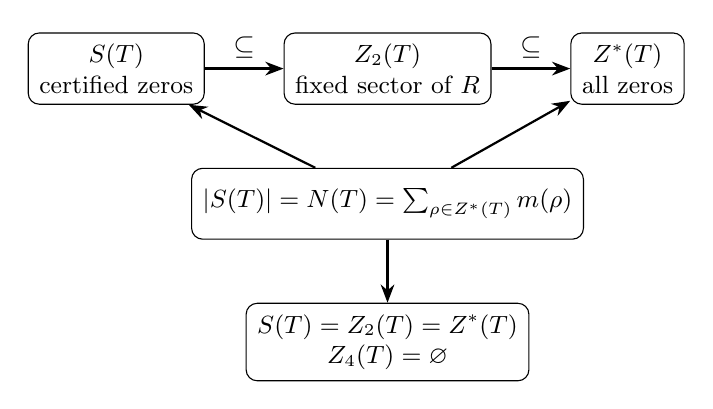
\begin{tikzpicture}[>=Stealth,node distance=8mm and 10mm,
 box/.style={draw,rounded corners,align=center,minimum height=9mm,inner sep=4pt,font=\small}]
\node[box] (s) {$S(T)$\\certified zeros};
\node[box,right=of s] (z2) {$Z_2(T)$\\fixed sector of $R$};
\node[box,right=of z2] (zs) {$Z^*(T)$\\all zeros};
\draw[->,thick] (s) -- node[above] {$\subseteq$} (z2);
\draw[->,thick] (z2) -- node[above] {$\subseteq$} (zs);
\node[box,below=of z2] (count) {$|S(T)|=N(T)=\sum_{\rho\in Z^*(T)}m(\rho)$};
\draw[->,thick] (count) -- (s);
\draw[->,thick] (count) -- (zs);
\node[box,below=of count] (close) {$S(T)=Z_2(T)=Z^*(T)$\\$Z_4(T)=\varnothing$};
\draw[->,thick] (count) -- (close);
\end{tikzpicture}
\caption{Critical route by saturation. Inclusion of the certified zeros in the fixed sector, combined with saturation of the total zero count, forces equality of sets and excludes the complement $Z_4(T)$.}
\label{fig:saturation-route}
\end{figure}

\section{Checks and counterexamples}
\subsection{Zero on the critical line}
For $\rho=1/2+i\gamma$,
\[
\Delta_R=0,\qquad R(\rho)=\rho,
\]
and the geometric orbit is $F_2$.

\subsection{Hypothetical zero off the critical line}
For
\begin{equation}
 \rho=\frac12+\delta+i\gamma,\qquad\delta\neq0,
\end{equation}
one obtains
\begin{equation}
 \Delta_R=-2\delta\neq0,
\end{equation}
\begin{equation}
 R(\rho)=\frac12-\delta+i\gamma\neq\rho,
\end{equation}
and the complete orbit is $F_4$. This orbit respects the known symmetries; therefore symmetry alone does not exclude $F_4$.

\subsection{Multiple zero on $1/2$}
If a zero on the critical line has multiplicity $m>1$, the orbit geometry remains $F_2$ and $R(\rho)=\rho$. Multiplicity appears only in \eqref{eq:logder}. Hence geometric closure and simplicity are distinct concepts.

\subsection{Trivial zeros}
The trivial zeros $-2n$ belong to $\zeta$ but not to the zero set of $\xi$ defined in \eqref{eq:xi}. Moreover, the reflection $s\mapsto1-s$ sends $-2n$ to $1+2n$, which is not another zero of $\zeta$. They therefore do not participate in the $F_2/F_4$ families of nontrivial zeros.

\subsection{$F_4$ encoding control}
The scalar map $Q(F_2)=\gamma^2$ is reversible on critical families. If an $F_4$ family is parameterized by $(\delta,\gamma)$, projecting it only to $\gamma^2$ loses $\delta$ and ceases to be injective; a complex or two-dimensional code can retain that information. This check delineates which part of reversibility comes from the critical family and what additional information must be controlled in a generic orbit.

\section{Closure theorems and logical status}
\begin{theorem}[Critical characterization]
For any nontrivial zero $\rho$,
\begin{equation}
 \Re(\rho)=\frac12
 \iff R(\rho)=\rho
 \iff F(\rho)=C(\rho)
 \iff \Delta_R(\rho)=0.
\end{equation}
In the upper half-plane, these conditions are equivalent to the orbit under $R$ having a single geometric position.
\end{theorem}

\begin{theorem}[Global criterion equivalent to RH]
RH is equivalent to any of the statements
\begin{align}
 Z^*&\subseteq\operatorname{Fix}(R),\\
 \Delta_R(\rho)&=0\quad\forall\rho\in Z^*,\\
 |\operatorname{Orb}_R(\rho)|&=1\quad\forall\rho\in Z^*.
\end{align}
\end{theorem}

\begin{theorem}[Strengthened unit-cell criterion]\label{thm:unitcells}
The following statements are equivalent:
\begin{enumerate}[label=(\roman*)]
\item RH holds and all nontrivial zeros are simple.
\item For every nontrivial zero $\rho_n$ there exists a Jordan region $B_n$ whose boundary contains no zeros, such that $R(B_n)=B_n$, $\rho_n\in B_n$, and
\[
N(B_n)=\frac{1}{2\pi i}\oint_{\partial B_n}\frac{\xi'(s)}{\xi(s)}\,ds=1.
\]
The regions can be chosen locally without other zeros, and the collection covers the set of nontrivial zeros.
\end{enumerate}
\end{theorem}

\begin{proof}
(ii)$\Rightarrow$(i): by the argument principle, $N(B_n)=1$ implies a unique zero counted with multiplicity one. The invariance $R(B_n)=B_n$ forces the image $R(\rho_n)$ to remain in the same region; uniqueness gives $R(\rho_n)=\rho_n$, and Proposition~\ref{prop:residual} yields $\Re(\rho_n)=1/2$. This holds for every $n$, and each multiplicity is one.

(i)$\Rightarrow$(ii): under RH, every $\rho_n$ lies on the fixed line of $R$; under simplicity and discreteness of the zero set of the entire function $\xi$, there exists a sufficiently small disk centered at $\rho_n$ containing no other zeros. Since the center lies on $\Re(s)=1/2$, the disk can be chosen $R$-invariant. The argument principle then gives $N(B_n)=1$.
\end{proof}

\begin{scope}
Theorem~\ref{thm:unitcells} converts the universal problem into a precise geometric-analytic objective: certify, through the constructed architecture, the exhaustive collection of $R$-invariant cells with unit index. This condition is the connecting point among the graph, the argument principle, and the strengthened result RH plus simplicity.
\end{scope}

\section{Architectural families and ``isotopes'' as an analogy}
In the exploratory analysis, the term \emph{architectural isotope} was used only as an analogy: within the same graph architecture, one varies a parameter (for example, $\varepsilon$, mean degree, or block size) while preserving the construction rule. Formally, the object is a parameterized family
\begin{equation}
 \{\mathcal G_R(\varepsilon)\}_{\varepsilon\ge0}.
\end{equation}
The standard term is \emph{filtration}; ``isotope'' is not proposed as a new technical term.

\section{Computational reproducibility}
The minimal implementation requires:
\begin{enumerate}
\item an ordered list of $\gamma_n$;
\item the unfolding function \eqref{eq:unfold};
\item distance matrices $|x_i-x_j|$;
\item matrices $A(\varepsilon)$, $D(\varepsilon)$, and $L(\varepsilon)$;
\item a sweep over $\varepsilon$ and computation of $\beta_0$;
\item optionally, persistent-homology software such as GUDHI to verify the Vietoris--Rips persistence diagram.
\end{enumerate}
The supplementary code associated with this manuscript implements exactly these steps and reproduces Table \ref{tab:beta}.

\section{Discussion}
The method articulates three complementary levels. The universal argument is formulated on the analytic set $Z^*(T)$ and the count $N(T)$, whereas numerical lists of ordinates are reserved for the computational layer; this separation keeps logical exhaustivity independent of numerical verification. The symmetry graph is exact and algebraic: it identifies whether a given orbit belongs to $F_2$ or $F_4$. The proximity graph is topological-spectral: it quantifies clustering of the ordinates and their persistence scales. The operator representation links both languages through equivariance and commutation, while the generational structure organizes the transmission of information between primary families and secondary objects. Section~\ref{sec:correspondencia} extends this reading by comparing the scheme with independent spectral correspondences known in mathematical physics.

Secondary zeta functions over zeros are established objects in the literature; organizing their codes through persistence constitutes the methodological extension developed here. The unit-cell criterion further specifies a globally verifiable condition: when the architecture certifies $R(B_n)=B_n$ and $N(B_n)=1$ exhaustively, RH and simplicity follow simultaneously. Thus the orbital classification, the representation $P_R$, the Laplacian, and the argument principle are integrated into a single mathematical chain.

\section{Independent structural correspondence: two parallel lines of logic}\label{sec:correspondencia}

\subsection{Two constructions of different origin}
The method distinguishes two lines of construction that do not arise from the same mathematical question. The first is analytic-topological: it starts from Riemann's completed function, its involutions, and the organization of the zeros,
\begin{equation}\label{eq:lineaA}
 \xi(s)\;\longrightarrow\;R(s)=1-\overline{s}\;\longrightarrow\;
 \operatorname{Fix}(R)\;\longrightarrow\;P_R\;\longrightarrow\;L .
\end{equation}
The second is operator-spectral: it starts from a state space, a symmetry, and a generator of dynamics,
\begin{equation}\label{eq:lineaB}
 \mathcal H\;\longrightarrow\;\mathcal J\;\longrightarrow\;
 \operatorname{Fix}(\mathcal J)\;\longrightarrow\;\widehat H\;\longrightarrow\;
 \operatorname{Spec}(\widehat H).
\end{equation}
In the monopole extension of Section~\ref{sec:monopolo}, for example, $\mathcal J^2=I$ and $[\widehat H_M,\mathcal J]=0$. In the symmetry graph, $P_R^2=I$ and, when the action preserves the architecture, $[L,P_R]=0$. Thus the two lines admit the same abstract logical scheme:
\begin{equation}\label{eq:parallelpattern}
 \boxed{\text{involution}\;\to\;\text{fixed sector}\;\to\;\text{commutation}\;\to\;\text{spectral decomposition}.}
\end{equation}

\begin{figure}[H]
\centering
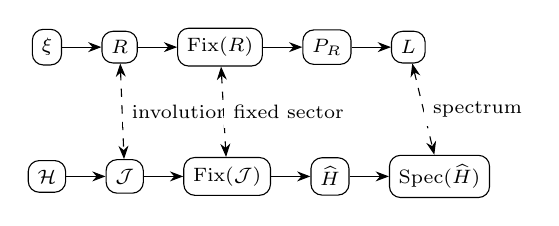
\begin{tikzpicture}[>=Stealth, node distance=7mm and 5mm, every node/.style={font=\scriptsize,align=center}]
\node[draw,rounded corners] (xi) {$\xi$};
\node[draw,rounded corners,right=of xi] (R) {$R$};
\node[draw,rounded corners,right=of R] (fixR) {$\operatorname{Fix}(R)$};
\node[draw,rounded corners,right=of fixR] (PR) {$P_R$};
\node[draw,rounded corners,right=of PR] (Lap) {$L$};
\draw[->] (xi)--(R); \draw[->] (R)--(fixR); \draw[->] (fixR)--(PR); \draw[->] (PR)--(Lap);

\node[draw,rounded corners,below=12mm of xi] (H) {$\mathcal H$};
\node[draw,rounded corners,right=of H] (J) {$\mathcal J$};
\node[draw,rounded corners,right=of J] (fixJ) {$\operatorname{Fix}(\mathcal J)$};
\node[draw,rounded corners,right=of fixJ] (Ham) {$\widehat H$};
\node[draw,rounded corners,right=of Ham] (Spec) {$\operatorname{Spec}(\widehat H)$};
\draw[->] (H)--(J); \draw[->] (J)--(fixJ); \draw[->] (fixJ)--(Ham); \draw[->] (Ham)--(Spec);

\draw[dashed,<->] (R)--node[right,fill=white] {involution} (J);
\draw[dashed,<->] (fixR)--node[right,fill=white] {fixed sector} (fixJ);
\draw[dashed,<->] (Lap)--node[right,fill=white] {spectrum} (Spec);
\end{tikzpicture}
\caption{Two parallel lines of logic. The upper row represents the analytic-graph construction associated with Riemann; the lower row, an operator-spectral construction. Dashed lines indicate architectural correspondences, not physical identity between the objects.}
\label{fig:parallel-lines}
\end{figure}

\subsection{Independent precedent: Riemann, random matrices, and quantum spectra}
The appearance of a common structure between number theory and spectral physics has a precedent independent of the present method. Montgomery studied the pair correlation of zeros of the zeta function \cite{Montgomery1973}; Dyson recognized that the resulting statistical form coincided with the eigenvalue correlation of random Hermitian matrices, a historical connection documented by the Institute for Advanced Study \cite{IASDyson}. Random-matrix theory had been developed in nuclear physics to describe statistical regularities of complex spectra, and the Bohigas--Giannoni--Schmit conjecture later related spectral fluctuations of quantum-chaotic systems to random-matrix ensembles \cite{BGS1984}. The DLMF explicitly records analogies between the distribution of the zeros of $\zeta$ and semiclassical quantum eigenvalues, as well as the Hilbert--P\'olya program \cite{DLMFphysical}.

This precedent is conceptually relevant because it shows that two disciplines built from different questions can converge on common spectral laws without one having been defined from the other. In the language of the present work, that convergence motivates the study not only of numerical coincidences, but of morphisms that preserve relations.

\subsection{Principle of structural correspondence}
Let $\mathcal A$ be an analytic architecture and $\mathcal G$ a graph architecture. We say that a \emph{structural correspondence} exists with respect to the involutions $R$ and $P$ if there is a map $Q:\mathcal A\to\mathcal G$ preserving the action,
\begin{equation}\label{eq:structcorr}
 \boxed{Q\circ R=P\circ Q.}
\end{equation}
If, in addition, $P$ is a graph automorphism, then
\begin{equation}\label{eq:structcorrLap}
 P^2=I,\qquad [L,P]=0,
\end{equation}
and the space can be decomposed into eigensectors of $P$. For the Riemann representation developed in this manuscript,
\begin{equation}
 P=P_R,\qquad Q(\operatorname{Fix}R)=\operatorname{Fix}(P_R)\cap Q(Z^*).
\end{equation}
The correspondence does not require identifying physical objects with analytic objects. It requires preservation of the essential relations. Accordingly, the mathematical content of the comparison lies in commutativity of the diagrams and coincidence of the architecture of invariants, not in a semantic equality among ``zero'', ``particle'', ``mode'', or ``state''.

\subsection{Interpretation for structures not directly accessible to visual observation}
In submicroscopic physics, elementary and collective degrees of freedom are not characterized by direct visual observation, but through detector responses, transition amplitudes, energy distributions, and spectra. The monopole mode provides a concrete example: the collective radial coordinate is not observed as a macroscopic sphere that literally ``breathes'', but is reconstructed through the response strength associated with an operator such as $\widehat M_{\rm IS0}$ and its spectral excitations. Analogously, Riemann zeros are studied through the analytic structure of $\xi$, its symmetries, counts, and correlations.

The structural statement of this work is therefore the following: architectures that appear to belong to different domains may constitute two parallel lines of logic when they preserve the same pattern of transformation and invariance. In condensed form,
\begin{equation}\label{eq:two-logic-lines}
 \boxed{
 \begin{array}{c}
 \text{analytic line: } R^2=I,\ [L,P_R]=0,\ \operatorname{Fix}(R),\\[1mm]
 \text{physical line: } \mathcal J^2=I,\ [\widehat H,\mathcal J]=0,\ \operatorname{Fix}(\mathcal J).
 \end{array}}
\end{equation}
The coincidence of form is not taken as proof of ontological identity; it is treated as a mathematically investigable object. When the two constructions are independent, persistence of the same pattern of involution, fixed point, commutation, and spectrum constitutes evidence of a structural correspondence and motivates the search for a more general common formalism.

\section{Asymptotic wave, matrix compression, and prime forcing}\label{sec:state-space}

\subsection{M\"obius amplitude and the exact action of reflection}
Introduce the dimensionless coordinate
\begin{equation}\label{eq:wcoord}
 w(\rho)=1-\frac1\rho=re^{i\theta}.
\end{equation}
For the critical reflection $R(\rho)=1-\overline\rho$, direct calculation gives
\begin{equation}\label{eq:wreflection}
 w(R\rho)=\frac1{\overline{w(\rho)}}=r^{-1}e^{i\theta}.
\end{equation}
\begin{proposition}[Exact Smith conjugacy]\label{prop:smith-conjugacy}
Let
\begin{equation}\label{eq:smith-centered-coordinate}
 z=2\rho-1,
 \qquad
 \Gamma(z)=\frac{z-1}{z+1}.
\end{equation}
For every $\rho\ne0$,
\begin{equation}\label{eq:smith-keiper-li-identity}
 \boxed{\ \Gamma(2\rho-1)=1-\frac1\rho=w(\rho)\ }.
\end{equation}
Moreover, $z(R\rho)=-\overline z$ and
$\Gamma(z(R\rho))=1/\overline{\Gamma(z)}$.  Consequently,
\begin{equation}\label{eq:smith-critical-boundary}
 \Re\rho=\frac12
 \quad\Longleftrightarrow\quad
 \Re z=0
 \quad\Longleftrightarrow\quad
 |\Gamma|=1.
\end{equation}
\end{proposition}
\begin{proof}
Substitution in the Smith bilinear map gives
\[
 \Gamma(2\rho-1)
 =\frac{(2\rho-1)-1}{(2\rho-1)+1}
 =\frac{\rho-1}{\rho}
 =1-\frac1\rho.
\]
The remaining statements follow from
$2(1-\overline\rho)-1=-\overline{(2\rho-1)}$ and direct conjugation.
\end{proof}

\begin{remark}[What Li's criterion confines]\label{rem:li-confinement}
With $w_\rho=1-1/\rho$, the Li coefficients can be written, under their
standard symmetric interpretation, as
\[
 \lambda_n=\sum_\rho\bigl[1-w_\rho^n\bigr].
\]
Li's theorem states that RH is equivalent to $\lambda_n\ge0$ for every
$n\ge1$ \cite{Li1997,BombieriLagarias}.  In the disk coordinate this is a
global positivity test equivalent to locating all transformed zeros on
$|w|=1$.  It detects an off-circle contribution through all orders $n$, but
it does not independently prove those inequalities; establishing them for
every $n$ is itself equivalent to RH.
\end{remark}
Thus $R$ preserves the angular coordinate and inverts the radial amplitude.  Moreover,
the central mechanism is binary: every generic state is treated together with its unique
reflected partner, forming the two-element orbit $(\rho,R\rho)$ and the reciprocal radial pair
$(r,r^{-1})$.  The different diagrams below are coordinate representations of this same
binary pair, not additional states.
At this stage RH is not an input.  The input is the established zero-set symmetry under $R$;
the target conclusion is reached only if an independently verified confinement criterion
forces every binary orbit into the fixed sector.  In schematic form,
\begin{equation}\label{eq:noncircular-rule}
 \boxed{\begin{gathered}
 \text{functional symmetry}+\text{independent confinement}\\
 \Longrightarrow\ \operatorname{Fix}(R)
 \ \Longleftrightarrow\ \Re\rho=\frac12.
 \end{gathered}}
\end{equation}
\begin{equation}\label{eq:wdelta}
 \Delta(\rho):=1-|w(\rho)|^2
 =\frac{2\beta-1}{\beta^2+\gamma^2},
 \qquad \rho=\beta+i\gamma,
\end{equation}
so
\begin{equation}\label{eq:wcircle}
 |w(\rho)|=1\quad\Longleftrightarrow\quad\beta=\frac12.
\end{equation}
Figure~\ref{fig:smith-sphere-map} displays the exact conjugacy
\eqref{eq:smith-keiper-li-identity} in the reflection-coefficient geometry associated with
the Smith chart~\cite{Smith1939}.  The chart is used here only as a
conformal visualization of the M\"obius coordinate; no electrical impedance model is assigned
to $\zeta$ or to its zeros.
In the centered coordinate $x=\beta-1/2$, the geometric center of the critical strip is
$x=0$, so the critical line is the central vertical axis.  The coordinate origin
$(x,y)=(0,0)$ corresponds to $\rho=1/2$ and is not a nontrivial zeta zero; the nontrivial
critical candidates have the form $\rho=1/2+i\gamma$ with $\gamma\ne0$.

\begin{figure}[H]
\centering
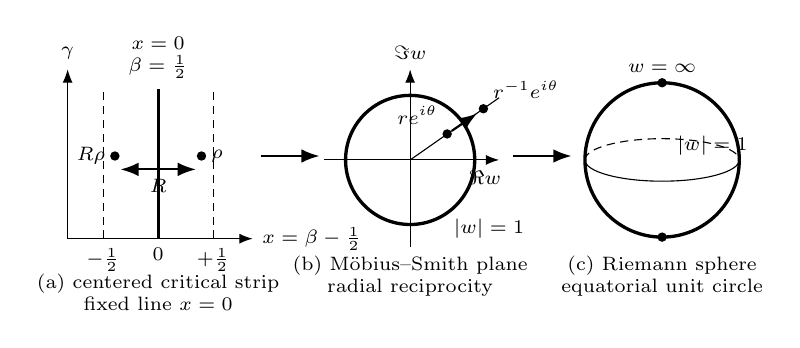
\begin{tikzpicture}[x=1cm,y=1cm,>=Latex,font=\scriptsize]
  % (a) Critical strip
  \draw[->] (0,0)--(2.35,0) node[right] {$x=\beta-\tfrac12$};
  \draw[->] (0,0)--(0,2.15) node[above] {$\gamma$};
  \draw[densely dashed] (0.45,0)--(0.45,1.90);
  \draw[very thick] (1.15,0)--(1.15,1.90)
    node[above,align=center] {$x=0$\\$\beta=\tfrac12$};
  \draw[densely dashed] (1.85,0)--(1.85,1.90);
  \node[below] at (0.45,0) {$-\tfrac12$};
  \node[below] at (1.15,0) {$0$};
  \node[below] at (1.85,0) {$+\tfrac12$};
  \fill (1.70,1.05) circle (1.7pt) node[right] {$\rho$};
  \fill (0.60,1.05) circle (1.7pt) node[left] {$R\rho$};
  \draw[<->,thick] (0.67,0.88)--(1.63,0.88) node[midway,below] {$R$};
  \node[align=center] at (1.15,-0.68) {(a) centered critical strip\\fixed line $x=0$};

  % Möbius map
  \draw[->,thick] (2.45,1.05)--(3.20,1.05);

  % (b) Smith/reflection-coefficient plane
  \coordinate (C) at (4.35,1.00);
  \draw[->] (3.25,1.00)--(5.48,1.00);
  \node[below] at (5.30,0.98) {$\Re w$};
  \draw[->] (4.35,-0.10)--(4.35,2.15) node[above] {$\Im w$};
  \draw[very thick] (C) circle (0.82);
  \node[below right] at (4.78,0.38) {$|w|=1$};
  \draw[thin] (C)--(5.48,1.79);
  \fill (4.82,1.33) circle (1.7pt) node[above left] {$re^{i\theta}$};
  \fill (5.28,1.65) circle (1.7pt) node[above right] {$r^{-1}e^{i\theta}$};
  \draw[->,thick] (4.88,1.37)--(5.20,1.59);
  \node[align=center] at (4.35,-0.48) {(b) M\"obius--Smith plane\\radial reciprocity};

  % Compactification
  \draw[->,thick] (5.65,1.05)--(6.40,1.05);

  % (c) Riemann sphere
  \coordinate (S) at (7.55,1.00);
  \draw[very thick] (S) circle (0.98);
  \draw (6.57,1.00) arc[start angle=180,end angle=360,x radius=0.98,y radius=0.27];
  \draw[densely dashed] (6.57,1.00) arc[start angle=180,end angle=0,x radius=0.98,y radius=0.27];
  \fill (7.55,1.98) circle (1.7pt) node[above] {$w=\infty$};
  \fill (7.55,0.02) circle (1.7pt);
  \node[right] at (7.62,1.18) {$|w|=1$};
  \node[align=center] at (7.55,-0.48) {(c) Riemann sphere\\equatorial unit circle};
\end{tikzpicture}
\caption{Three representations of one binary mechanism: critical strip, M\"obius--Smith
plane, and Riemann sphere.  The pair $\rho,R\rho$ maps to points of radii $r,r^{-1}$ on the same ray.
The critical line maps exactly to the unit circle, represented as the equator after
compactification.  The point $w=\infty$ is geometric and is not an arithmetic zero or a
substitute for finite-height exhaustion.}
\label{fig:smith-sphere-map}
\end{figure}

The raw residual in \eqref{eq:wdelta} tends to zero as $|\rho|\to\infty$ even if
$\beta\ne1/2$.  This is a loss of scale, not critical closure.  The normalized residual
\begin{equation}\label{eq:normalizedresidual}
 (\beta^2+\gamma^2)\Delta(\rho)=2\beta-1
\end{equation}
retains the transverse information.  Infinity is handled by finite exhaustion
$T_j\to\infty$ and never as an arithmetic value; in particular no argument uses $0/0$.

For $w\ne0$ and integers $n\ne m$, exact two-harmonic cancellation satisfies
\begin{equation}\label{eq:harmoniccancel}
 w^n+w^m=0
 \quad\Longrightarrow\quad
 r=1,
 \qquad
 \theta=\frac{(2k+1)\pi}{n-m}.
\end{equation}
Equation \eqref{eq:harmoniccancel} is an angular gate at discrete phases.  It does not assert
that every zero must activate that gate.

\subsection{Buckingham reduction and the natural parameter $K$}
Let $u$ denote the independent scale variable and write the generalized mode
\begin{equation}\label{eq:modeau}
 q_\rho(u)=A_0e^{au}e^{i(\gamma u+\phi)},
 \qquad a=\beta-\frac12.
\end{equation}
In the dimensional analogue, $[A]=[A_0]=L$, $[a]=[\gamma]=T^{-1}$ and $[u]=T$.
Five variables built from two base dimensions yield three independent Buckingham groups.
A convenient choice is
\begin{equation}\label{eq:PiGroups}
 \Pi_1=\frac A{A_0},
 \qquad \Pi_2=\tau=\gamma u,
 \qquad \Pi_3=K_\rho=\frac a\gamma
 =\frac{\beta-1/2}{\gamma}.
\end{equation}
Accordingly,
\begin{equation}\label{eq:reducedmode}
 \frac{q_\rho}{A_0}=e^{K_\rho\tau}e^{i(\tau+\phi)}.
\end{equation}
The critical reflection preserves $\gamma$ and sends $a\mapsto-a$; hence
\begin{equation}\label{eq:Kreflection}
 K_\rho\mapsto-K_\rho.
\end{equation}
Over one phase cycle, the reflected gains are
\begin{equation}\label{eq:cyclegains}
 G_+=e^{2\pi K_\rho},
 \qquad G_-=e^{-2\pi K_\rho},
 \qquad G_+G_-=1.
\end{equation}

\begin{theorem}[Bilateral cycle-passivity criterion]\label{thm:cycle-passivity}
If the two reflected branches associated with a zero are independently realized in a common
forward-passive architecture, then $G_+\le1$ and $G_-\le1$ imply
\[
 K_\rho=0\qquad\text{and hence}\qquad\Re\rho=\frac12.
\]
\end{theorem}
\begin{proof}
Two positive reciprocal numbers cannot both be at most one unless both equal one.
Equation \eqref{eq:cyclegains} therefore gives $e^{2\pi K_\rho}=1$, hence $K_\rho=0$.
Since a nontrivial zero has $\gamma\ne0$, \eqref{eq:PiGroups} gives $\beta=1/2$.
\end{proof}

The theorem is an exact confinement implication.  Its spectral use requires the two branches
to have been realized from arithmetic data without presupposing their transverse location.

\subsection{Three-dimensional state and recurrence}
The one-dimensional ordered data become a three-dimensional trajectory by retaining the
longitudinal unfolded coordinate and the two quadratures of the complex amplitude:
\begin{equation}\label{eq:state3d}
 \mathbf S_n^{(3)}=(x_n,X_n,Y_n)
 =\bigl(x_n,A_n\cos\phi_n,A_n\sin\phi_n\bigr),
\end{equation}
where $x_n=\overline N(\gamma_n)$ is defined by \eqref{eq:unfold}.  Put
\begin{equation}\label{eq:gapandphase}
 d_n=x_{n+1}-x_n,
 \qquad \Delta\tau_n=2\pi d_n.
\end{equation}
The factor $2\pi$ makes one unit of unfolded separation correspond to one phase cycle.  The
state recurrence is
\begin{align}
 A_{n+1}&=A_ne^{2\pi K_nd_n},\label{eq:amprecurrence}\\
 \phi_{n+1}&=\phi_n+2\pi d_n\pmod{2\pi},\label{eq:phaserecurrence}\\
 x_{n+1}&=x_n+d_n.\label{eq:xrecurrence}
\end{align}
Equivalently, on the transverse plane,
\begin{equation}\label{eq:matrixtransition}
 \binom{X_{n+1}}{Y_{n+1}}
 =e^{2\pi K_nd_n}
 \begin{pmatrix}
 \cos(2\pi d_n)&-\sin(2\pi d_n)\\
 \sin(2\pi d_n)& \cos(2\pi d_n)
 \end{pmatrix}
 \binom{X_n}{Y_n}.
\end{equation}
For $K_n=0$, $X_n^2+Y_n^2=A_0^2$ and the states lie on an irregular helix of fixed radius.
For $K_n\ne0$, the radius expands or contracts, while reflection reverses the radial rate.

\subsection{Paired Smith coordinates and the quaternionic hypersphere}
\label{subsec:quaternion-smith}
The direct and reflected Smith coordinates can be assembled without loss into one quaternion.
Write
\begin{equation}\label{eq:quaternion-algebra}
 \mathbb H=\{a+bi+cj+dk:a,b,c,d\in\mathbb R\},
 \qquad i^2=j^2=k^2=ijk=-1.
\end{equation}
The oriented products satisfy
\begin{equation}\label{eq:quaternion-products}
 ij=k,\qquad jk=i,\qquad ki=j,
 \qquad ji=-k,\qquad kj=-i,\qquad ik=-j.
\end{equation}
Thus multiplication is associative but not commutative.  Quaternionic conjugation and norm are
\begin{equation}\label{eq:quaternion-norm}
 \overline q=a-bi-cj-dk,
 \qquad
 \|q\|^2=q\overline q=a^2+b^2+c^2+d^2.
\end{equation}
The unit quaternions form
\begin{equation}\label{eq:S3-unit-quaternions}
 S^3=\{q\in\mathbb H:\|q\|=1\},
\end{equation}
whose axial points are $\{\pm1,\pm i,\pm j,\pm k\}$.  The zero quaternion is the center of
$\mathbb R^4$, not a point of $S^3$; in particular it has no multiplicative inverse.

Let
\begin{equation}\label{eq:paired-smith-coordinates}
 z_D(\rho)=w(\rho),\qquad
 z_A(\rho)=w(R\rho)=\frac{1}{\overline{w(\rho)}}.
\end{equation}
The paired quaternionic lift is
\begin{equation}\label{eq:quaternion-lift}
 \Phi(\rho)=Q_\rho:=z_D(\rho)+z_A(\rho)j.
\end{equation}
If $z_D=a+bi$ and $z_A=c+di$, then, using $ij=k$,
\begin{equation}\label{eq:quaternion-four-coordinates}
 Q_\rho=a+bi+cj+dk,
 \qquad
 \|Q_\rho\|^2=|z_D|^2+|z_A|^2.
\end{equation}
Because $w(s)=1-1/s$ has inverse $w^{-1}(z)=1/(1-z)$, the first component already recovers
$\rho$.  Hence $\Phi$ is injective on the nontrivial zero set.  The two complex components in
\eqref{eq:paired-smith-coordinates} are linked by reflection and are therefore not independent:
the image of $\Phi$ is a two-real-dimensional embedded surface in $\mathbb H$, represented by
four real coordinates, rather than all of $\mathbb R^4$.

Define the real-linear component-exchange involution
\begin{equation}\label{eq:quaternion-exchange}
 \mathcal P(z_1+z_2j)=z_2+z_1j,
 \qquad \mathcal P^2=I.
\end{equation}
Since $R^2=I$, the lift is equivariant:
\begin{equation}\label{eq:quaternion-equivariance}
 \boxed{\ \Phi(R\rho)=\mathcal P\Phi(\rho)\ }.
\end{equation}
Thus applying critical reflection before the lift is identical to exchanging the two Smith
components after the lift.  Moreover,
\begin{align}
 \mathcal P Q_\rho=Q_\rho
 &\iff z_D(\rho)=z_A(\rho)\notag\\
 &\iff w(\rho)=\frac1{\overline{w(\rho)}}\notag\\
 &\iff |w(\rho)|=1\notag\\
 &\iff \Re\rho=\frac12.\label{eq:quaternion-fixed-chain}
\end{align}
The corresponding nonnegative quaternionic defect is
\begin{equation}\label{eq:quaternion-defect}
 \mathcal D_{\mathbb H}(\rho)
 :=\|Q_\rho-\mathcal P Q_\rho\|^2
 =2|z_D(\rho)-z_A(\rho)|^2\ge0,
\end{equation}
and therefore
\begin{equation}\label{eq:quaternion-defect-zero}
 \boxed{\ \mathcal D_{\mathbb H}(\rho)=0
 \iff R\rho=\rho
 \iff \Re\rho=\frac12\ }.
\end{equation}

For $Q_\rho\ne0$ its scale and unit orientation separate uniquely as
\begin{equation}\label{eq:quaternion-polar}
 Q_\rho=r_\rho U_\rho,
 \qquad r_\rho=\|Q_\rho\|>0,
 \qquad U_\rho=Q_\rho/\|Q_\rho\|\in S^3.
\end{equation}
Writing $z_D=w=a+bi$ and $z_A=x_S+iy_S$, define the normalized coordinates
\begin{equation}\label{eq:normalized-smith-quaternion-coordinates}
 \widehat w=\frac{w}{r_\rho},
 \qquad
 \widehat x_S=\frac{x_S}{r_\rho},
 \qquad
 \widehat y_S=\frac{y_S}{r_\rho},
 \qquad
 r_\rho^2=|w|^2+x_S^2+y_S^2.
\end{equation}
Then the unit quaternion has the one-complex-plus-two-real form
\begin{equation}\label{eq:one-complex-two-real-quaternion}
 U_\rho=\widehat w+\widehat x_Sj+\widehat y_Sk
\end{equation}
and satisfies the hypersphere equation
\begin{equation}\label{eq:complex-S3-equation}
 \boxed{\ |\widehat w|^2+\widehat x_S^2+\widehat y_S^2=1\ }.
\end{equation}
Since $\widehat w=\widehat a+\widehat b i$, equation~\eqref{eq:complex-S3-equation}
is exactly
\begin{equation}\label{eq:real-S3-equation}
 \widehat a^2+\widehat b^2+\widehat x_S^2+\widehat y_S^2=1.
\end{equation}
Thus the complex coordinate supplies two real components and the remaining Smith component
supplies the other two.  When normalized coordinates are understood, hats may be suppressed
and the same equation is written $|w|^2+x_S^2+y_S^2=1$.  Retaining $r_\rho$ makes the
normalization reversible and prevents radial scale from being discarded.
This is the quaternionic analogue of $z=re^{i\theta}$.  General orientation-preserving
four-dimensional rotations with a uniform scale have the two-sided form
\begin{equation}\label{eq:quaternion-two-sided-rotation}
 x\longmapsto \lambda u x v^{-1},
 \qquad \lambda>0,\quad u,v\in S^3,
\end{equation}
where the left and right actions commute.  Equivalently,
$\operatorname{Spin}(4)\cong S^3_L\times S^3_R$ and
$SO(4)\cong(S^3_L\times S^3_R)/\{(1,1),(-1,-1)\}$.

The dimensional representations retain different parts of the same state.  The complex
Smith plane gives the two-dimensional coordinate $z_D$; the quaternion gives the four real
coordinates in~\eqref{eq:quaternion-four-coordinates}; and the unit orientation admits the
stereographic coordinate
\begin{equation}\label{eq:S3-stereographic}
 \pi(a+bi+cj+dk)=\frac{(b,c,d)}{1-a}\in\mathbb R^3,
 \qquad a\ne1.
\end{equation}
A second stereographic chart based at $-1$ covers the excluded pole.  Finally, the Cantor
pairing of Section~\ref{sec:cantor-closure} gives a reversible one-dimensional address for
the discretely indexed occupied cell.  The one-dimensional correspondence applies to cell
indices, not to an uncountable continuum of quaternionic points.

\begin{corollary}[Quaternionic form of unit-cell uniqueness]
\label{cor:quaternion-unit-cell}
Let $\{B_\nu\}$ be an exhaustive collection of Jordan regions for the nontrivial zeros, with
zero-free boundaries, such that $R(B_\nu)=B_\nu$ and
\begin{equation}\label{eq:quaternion-unit-index}
 N_{\rm mult}(B_\nu)
 =\frac{1}{2\pi i}\oint_{\partial B_\nu}
   \frac{\xi'(s)}{\xi(s)}\,ds=1.
\end{equation}
Then every lifted zero is fixed by $\mathcal P$, every nontrivial zero lies on the critical
line, and every nontrivial zero is simple.
\end{corollary}
\begin{proof}
If $\rho\in B_\nu$, zero-set symmetry and invariance give $R\rho\in B_\nu$.  The unit index
counts one zero with multiplicity, hence $R\rho=\rho$ and the multiplicity is one.
Equation~\eqref{eq:quaternion-equivariance} gives
$\mathcal P Q_\rho=Q_\rho$, and~\eqref{eq:quaternion-fixed-chain} gives
$\Re\rho=1/2$.  Exhaustiveness applies this conclusion to every nontrivial zero.
\end{proof}

\begin{theorem}[Quaternionic closure by finite saturation]
\label{thm:quaternion-saturation}
Fix $T<\infty$ with zero-free horizontal boundary.  Let
$\{B_\nu(T)\}_{\nu=1}^{M(T)}$ be pairwise zero-disjoint Jordan regions satisfying
\begin{equation}\label{eq:quaternion-certified-cells}
 R(B_\nu(T))=B_\nu(T),
 \qquad
 \frac{1}{2\pi i}\oint_{\partial B_\nu(T)}
       \frac{\xi'(s)}{\xi(s)}\,ds=1.
\end{equation}
Let $S(T)$ be the set of their certified zeros and put
\begin{equation}\label{eq:quaternion-certified-lifts}
 \widehat S(T)=\Phi(S(T)),
 \qquad
 \widehat Z(T)=\Phi(Z^*(T)).
\end{equation}
If the independently computed total count is saturated,
\begin{equation}\label{eq:quaternion-saturation-count}
 M(T)=N(T),
\end{equation}
then
\begin{equation}\label{eq:quaternion-saturation-conclusion}
 \widehat S(T)=\widehat Z(T)
 \subseteq\operatorname{Fix}(\mathcal P),
 \qquad Z_4(T)=\varnothing,
\end{equation}
and every nontrivial zero below $T$ is simple and lies on $\Re s=1/2$.
If the same construction and equality hold along an exhaustive sequence
$T_m\to\infty$, then RH holds and every nontrivial zero is simple.
\end{theorem}
\begin{proof}
Equation~\eqref{eq:quaternion-certified-cells} and
Corollary~\ref{cor:quaternion-unit-cell} give
$S(T)\subseteq Z_2(T)$ and show that every element of $S(T)$ is simple.  Hence
\[
 |S(T)|=M(T)=N(T)=\sum_{\rho\in Z^*(T)}m(\rho).
\]
The finite-set inequalities
\[
 |S(T)|\le |Z^*(T)|\le
 \sum_{\rho\in Z^*(T)}m(\rho)
\]
therefore have equal endpoints.  Thus $S(T)=Z^*(T)$ and every multiplicity equals one.
Since $\Phi$ is injective, applying it preserves this equality and gives
$\widehat S(T)=\widehat Z(T)$.  Every certified lift is fixed by $\mathcal P$ through
\eqref{eq:quaternion-equivariance}, so~\eqref{eq:quaternion-saturation-conclusion} follows.
Finally, every zero has finite ordinate; taking the increasing union over an exhaustive
sequence $T_m$ yields the global statement.
\end{proof}

Corollary~\ref{cor:quaternion-unit-cell} is the two-chart quaternionic representation of
Theorem~\ref{thm:unitcells}.  It does not infer the unit index from coordinate uniqueness:
the contour value in~\eqref{eq:quaternion-unit-index} must be certified by a cell construction
independent of RH and simplicity.  Once that certification is exhaustive, the Smith,
quaternionic, graph, and cell descriptions form the same fixed-point conclusion.
Theorem~\ref{thm:quaternion-saturation} applies exactly the finite counting method of
Theorem~\ref{thm:saturation}; the lift preserves the closure but does not by itself establish
the saturation identity~\eqref{eq:quaternion-saturation-count}.

\subsection{Asymptotic wave, two-axis compression, and the law of commutation}
\label{subsec:asymptotic-matrix}
The matrix mechanism is obtained from two scalar coordinates, one for each axis.  Write
\begin{equation}\label{eq:two-axis-coordinate}
 x=\beta-\frac12,\qquad y=\gamma,\qquad
 \mathbf a(\rho)=\binom{x}{y}.
\end{equation}
The generalized amplitude--phase mode in~\eqref{eq:modeau} is therefore the asymptotic wave
\begin{equation}\label{eq:asymptotic-wave}
 \Psi_\rho(u)=A_0e^{xu}e^{i(yu+\phi)},\qquad u\ge0.
\end{equation}
The sign of $x$ gives growth or decay as $u\to+\infty$, while $x=0$ gives neutral
amplitude.  No value is assigned at infinity: the asymptotic statement is the family of
finite-$u$ estimates followed by the limit $u\to+\infty$.

The critical reflection $R(\rho)=1-\overline\rho$ is represented by
\begin{equation}\label{eq:Jcritical}
 \mathbf a(R\rho)=J_c\mathbf a(\rho),\qquad
 J_c=\begin{pmatrix}-1&0\\0&1\end{pmatrix},\qquad J_c^2=I_2.
\end{equation}
Thus the $x$ operation is $x\mapsto-x$ and the $y$ operation is $y\mapsto y$.
The matrix is their direct-sum representation, not a replacement of either scalar axis.
The corresponding complementary projectors are
\begin{equation}\label{eq:critical-projectors}
 P_{\parallel}=\frac{I_2+J_c}{2}
   =\begin{pmatrix}0&0\\0&1\end{pmatrix},\qquad
 P_{\perp}=\frac{I_2-J_c}{2}
   =\begin{pmatrix}1&0\\0&0\end{pmatrix}.
\end{equation}
They satisfy
\begin{equation}\label{eq:projector-algebra}
 P_{\parallel}+P_{\perp}=I_2,qquad
 P_{\parallel}P_{\perp}=P_{\perp}P_{\parallel}=O_2,qquad
 \operatorname{rank}P_{\parallel}=\operatorname{rank}P_{\perp}=1.
\end{equation}
Consequently, critical compression removes only the transverse coordinate:
\begin{equation}\label{eq:matrix-defect}
 \mathcal C(\rho)=\|P_{\perp}\mathbf a(\rho)\|^2=x^2,qquad
 \mathcal C(\rho)=0\iff\Re\rho=\frac12.
\end{equation}

Total nodal cancellation is a different involution.  If
$\psi=F e^{iG}$ and its paired branch has equal amplitude and phase opposition,
$\psi'=F e^{i(G+\pi)}=-\psi$, then the real two-component amplitude vector is acted on by
\begin{equation}\label{eq:Jnodal}
 J_n=-I_2,qquad J_n^2=I_2,qquad I_2+J_n=O_2,qquad
 \operatorname{rank}(O_2)=0.
\end{equation}
Hence $(I_2+J_n)\mathbf v=O_2\mathbf v=\mathbf0$ is the matrix form of
$\psi+\psi'=0$.  The null and identity matrices obey
\begin{equation}\label{eq:null-identity-laws}
 A+O_2=A,qquad AO_2=O_2A=O_2,qquad AI_2=I_2A=A.
\end{equation}
In particular, $O_2\ne I_2$.  Equation~\eqref{eq:Jnodal} has rank zero after summation,
whereas critical reflection in~\eqref{eq:Jcritical} has the rank-one fixed sector
$\operatorname{im}P_{\parallel}$.  This is the precise separation between nodal annihilation
and confinement to the critical line.

For compatibility with the monopolar nodal formulation, let $X$ denote the selected
transverse observable and let $\operatorname{Tr}_q$ be the trace functional specified on its
domain.  The flattening condition
\begin{equation}\label{eq:trace-flattening}
 \operatorname{Tr}_q[X^2]=0
\end{equation}
records that no transverse quadratic residue remains in that channel.  When
$\operatorname{Tr}_q$ is a positive Hilbert-space trace and $X=X^*$, it forces $X=0$ on the
traced sector.  For an indefinite, projected, or renormalized functional, its domain and
positivity must be supplied separately.  The phase cancellation in~\eqref{eq:Jnodal} follows
from equal amplitude and opposition by $\pi$; equation~\eqref{eq:trace-flattening} is the
geometric flattening statement and is not silently used as a substitute for that algebra.

\begin{theorem}[Law of commutation]\label{thm:commutation-law}
The critical and nodal involutions, and all polynomials in them, commute.  Explicitly,
\begin{equation}\label{eq:matrix-commutation-law}
 [J_c,J_n]=O_2,qquad
 [P_{\parallel},P_{\perp}]=O_2,qquad
 P_{\parallel}P_{\perp}=O_2.
\end{equation}
If $P_R$ is the graph automorphism induced by the same critical reflection, then
\begin{equation}\label{eq:full-commutation-law}
 P_R^2=I,qquad [L,P_R]=0,qquad
 \left[L,\frac{I\pm P_R}{2}\right]=0.
\end{equation}
Thus decomposition into reflected symmetry sectors can be performed before or after the
Laplacian action; the observable result is unchanged.
\end{theorem}
\begin{proof}
$J_n=-I_2$ commutes with every $2\times2$ matrix.  The matrices in
\eqref{eq:critical-projectors} are diagonal, giving~\eqref{eq:matrix-commutation-law}
directly.  The graph identities follow from $LP_R=P_RL$ and linearity.
\end{proof}

\begin{theorem}[Finite-height injective confinement criterion]
\label{thm:injective-confinement}
Let $T<\infty$ and let
$\mathcal A_T:Z^*(T)\to\mathcal K_T$ be an injective cell representation satisfying the
commutative invariance
\begin{equation}\label{eq:cell-commutation}
 \mathcal A_T\circ R=\mathcal A_T
 \quad\text{on }Z^*(T).
\end{equation}
Then $Z_4(T)=\varnothing$.  If the same construction is established for every finite $T$,
then all nontrivial zeros lie on the critical line.  Bijectivity is sufficient, but only its
injective part is used.
\end{theorem}
\begin{proof}
For $\rho\in Z^*(T)$, equation~\eqref{eq:cell-commutation} gives
$\mathcal A_T(R\rho)=\mathcal A_T(\rho)$.  Injectivity gives $R\rho=\rho$; by
Proposition~\ref{prop:residual}, this is equivalent to $x=0$.  Hence no $F_4$ orbit occurs
below $T$.  Every zero has finite ordinate, so finite exhaustion yields the universal statement.
\end{proof}

The criterion identifies exactly what must be verified by the construction: invariance and
injectivity may not be inferred merely from the uniqueness of the scalar value zero.  In the
M\"obius--Smith coordinate $w=1-1/\rho$, the same fixed sector is $|w|=1$ by
\eqref{eq:wcircle}; the Smith chart is its planar conformal representation, while adjoining
the point at infinity gives the Riemann sphere rather than a M\"obius band or torus.

\begin{figure}[H]
\centering
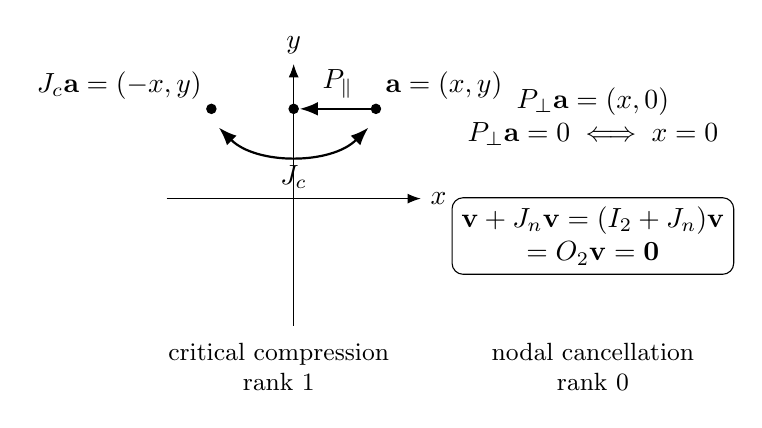
\begin{tikzpicture}[>=Latex,scale=0.95]
  \draw[->] (-4,0)--(-0.6,0) node[right] {$x$};
  \draw[->] (-2.3,-1.7)--(-2.3,1.8) node[above] {$y$};
  \fill (-1.2,1.2) circle (2pt) node[above right] {$\mathbf a=(x,y)$};
  \fill (-3.4,1.2) circle (2pt) node[above left] {$J_c\mathbf a=(-x,y)$};
  \draw[<->,thick] (-3.3,0.95) .. controls (-2.8,0.45) and (-1.8,0.45) .. (-1.3,0.95)
    node[midway,below] {$J_c$};
  \fill (-2.3,1.2) circle (2pt);
  \draw[->,thick] (-1.2,1.2)--(-2.22,1.2) node[midway,above] {$P_{\parallel}$};
  \node[align=center] at (1.7,1.1) {$P_{\perp}\mathbf a=(x,0)$\\$P_{\perp}\mathbf a=0\iff x=0$};
  \node[draw,rounded corners,align=center] at (1.7,-0.5)
    {$\mathbf v+J_n\mathbf v=(I_2+J_n)\mathbf v$\\$=O_2\mathbf v=\mathbf0$};
  \node[align=center,font=\small] at (-2.5,-2.25)
    {critical compression\\rank $1$};
  \node[align=center,font=\small] at (1.7,-2.25)
    {nodal cancellation\\rank $0$};
\end{tikzpicture}
\caption{Two operations that must remain distinct.  Critical reflection cancels the transverse
defect while preserving the ordinate; phase-opposed nodal inversion cancels both amplitude
components.}
\label{fig:matrix-compression}
\end{figure}

\subsection{Fourth arithmetic coordinate and fifth diagnostic coordinate}
Euler's logarithmic derivative supplies the prime-power frequencies and weights
\begin{equation}\label{eq:primechannels}
 -\frac{\zeta'(s)}{\zeta(s)}
 =\sum_p\sum_{m\ge1}(\log p)p^{-ms},
 \qquad
 \omega_{p,m}=m\log p,
 \qquad
 a_{p,m}=\frac{\log p}{p^{m/2}}.
\end{equation}
At $\rho=1/2+a+i\gamma$ the direct and reflected prime factors are
\begin{align}
 p^{-m\rho}&=p^{-m/2}e^{-ma\log p}e^{-im\gamma\log p},\\
 p^{-mR(\rho)}&=p^{-m/2}e^{ma\log p}e^{-im\gamma\log p}.
\end{align}
They have equal phase and reciprocal normalized amplitudes.  Their symmetric and
antisymmetric combinations are proportional to $\cosh(ma\log p)$ and
$-\sinh(ma\log p)$, respectively; the antisymmetric channel vanishes at $a=0$.

\subsection{Signed square-root defect and its global sum}
Fix finite nonempty cutoffs $P\ge2$ and $M\ge1$.  Define the normalized positive
prime-power weights as follows:
\begin{equation}\label{eq:normalized-prime-defect-weights}
 \widetilde a_{p,m}
 =\frac{a_{p,m}}
 {\displaystyle\sum_{q\le P}\sum_{1\le n\le M}a_{q,n}},
 \qquad
 \sum_{p\le P}\sum_{m\le M}\widetilde a_{p,m}=1.
\end{equation}
For $\rho=1/2+a+i\gamma$, define the squared separation of the reciprocal
amplitude branches by
\begin{align}
 \mathcal E_{P,M}(\rho)
 &:=\sum_{p\le P}\sum_{m\le M}\widetilde a_{p,m}
 \left|e^{ma\log p}-e^{-ma\log p}\right|^2\label{eq:prime-defect-energy-definition}\\
 &=4\sum_{p\le P}\sum_{m\le M}\widetilde a_{p,m}
 \sinh^2(ma\log p)\ge0.\label{eq:prime-defect-energy-sinh}
\end{align}
The phase $e^{-im\gamma\log p}$ has unit modulus and therefore disappears from
the squared separation.  Consequently distinct phase channels cannot cancel one
another in~\eqref{eq:prime-defect-energy-sinh}.

Solving the quadratic relation $d^2=\mathcal E_{P,M}$ gives the two real branches
\begin{equation}\label{eq:prime-defect-plus-minus-branches}
 \boxed{\quad
 \mathcal D^{\,\pm}_{P,M}(\rho)
 =\pm\sqrt{\mathcal E_{P,M}(\rho)}
 =\pm2\sqrt{\sum_{p\le P}\sum_{m\le M}
 \widetilde a_{p,m}\sinh^2(ma\log p)}\quad}.
\end{equation}
The principal square root is nonnegative; the symbol $\pm$ records the two
solutions of the quadratic relation.  To retain the orientation of the direct
state, set
\begin{equation}\label{eq:oriented-prime-defect}
 \mathcal D_{P,M}(\rho)
 :=\begin{cases}
 \operatorname{sgn}(a)\sqrt{\mathcal E_{P,M}(\rho)},&a\ne0,\\
 0,&a=0.
 \end{cases}
\end{equation}
Reflection sends $a\mapsto-a$.  Hence
\begin{equation}\label{eq:prime-defect-reflection-parity}
 \mathcal E_{P,M}(R\rho)=\mathcal E_{P,M}(\rho),
 \qquad
 \mathcal D_{P,M}(R\rho)=-\mathcal D_{P,M}(\rho).
\end{equation}

\begin{proposition}[Unique intersection of the signed prime branches]
\label{prop:prime-defect-unique-intersection}
For every $\rho=1/2+a+i\gamma$ and every finite nonempty pair of cutoffs
$P\ge2$, $M\ge1$,
\begin{equation}\label{eq:prime-defect-zero-chain}
 \boxed{\quad
 \mathcal D^{+}_{P,M}(\rho)=\mathcal D^{-}_{P,M}(\rho)
 \iff \mathcal E_{P,M}(\rho)=0
 \iff a=0
 \iff \Re\rho=\frac12.\quad}
\end{equation}
\end{proposition}
\begin{proof}
The two branches in~\eqref{eq:prime-defect-plus-minus-branches} are equal if and
only if their common nonnegative magnitude is zero.  Every summand in
\eqref{eq:prime-defect-energy-sinh} is nonnegative and every weight is positive,
so the sum vanishes if and only if $\sinh(ma\log p)=0$ for every included
prime-power channel.  Since $m\log p>0$ and $\sinh x=0$ only for $x=0$, this is
equivalent to $a=0$.
\end{proof}

For an admissible finite height $T$, sum the nonnegative squared defect over the
analytic zero set, with multiplicity:
\begin{align}\label{eq:global-summed-prime-defect}
 \mathfrak G_{P,M}(T)
 &:=\sum_{\rho\in Z^*(T)}m(\rho)\mathcal E_{P,M}(\rho)\\
 &=4\sum_{\rho\in Z^*(T)}m(\rho)
 \sum_{p\le P}\sum_{m\le M}\widetilde a_{p,m}
 \sinh^2\!\left(m(\Re\rho-\tfrac12)\log p\right).
\end{align}

\begin{theorem}[Global summed-defect criterion]
\label{thm:global-summed-prime-defect}
For every admissible finite height $T$ and every finite nonempty pair of cutoffs
$P\ge2$, $M\ge1$,
\begin{equation}\label{eq:global-summed-defect-equivalence}
 \boxed{\quad
 \mathfrak G_{P,M}(T)=0
 \iff Z_4(T)=\varnothing
 \iff \Re\rho=\frac12\quad(\rho\in Z^*(T)).\quad}
\end{equation}
Consequently, if $\mathfrak G_{P,M}(T_k)=0$ along an exhaustive sequence
$T_k\to\infty$ whose boundaries contain no zeros, then RH holds.
\end{theorem}
\begin{proof}
The set $Z^*(T)$ is finite and every multiplicity is positive.  Therefore the
finite sum of nonnegative terms in~\eqref{eq:global-summed-prime-defect} is zero
if and only if each $\mathcal E_{P,M}(\rho)$ is zero.  Proposition
\ref{prop:prime-defect-unique-intersection} then gives $\Re\rho=1/2$ for every
$\rho\in Z^*(T)$, which is equivalent to $Z_4(T)=\varnothing$.  The converse is
immediate.  Every nontrivial zero has finite ordinate, so exhaustion in height
gives the final implication.
\end{proof}

The ordinary algebraic sum of the two signed branches is identically zero,
\begin{equation}\label{eq:signed-branch-algebraic-cancellation}
 \mathcal D^{+}_{P,M}(\rho)+\mathcal D^{-}_{P,M}(\rho)=0,
\end{equation}
for every $a$; it expresses reflection symmetry and is not a confinement test.
The sum of squared magnitudes in~\eqref{eq:global-summed-prime-defect} is the
nonnegative quantity that detects transverse displacement.  Thus
Theorem~\ref{thm:global-summed-prime-defect} is an exact criterion: its universal
application requires deriving the stated zero value from arithmetic data rather
than inserting $a=0$ into the definition.

Using the same normalized weights, define
\begin{equation}\label{eq:Qlambda}
 Q_\Lambda(\gamma)
 =\sum_{p\le P}\sum_{m\le M}\widetilde a_{p,m}
 \mathbf 1_{\{\cos(m\gamma\log p)<0\}},
 \qquad 0\le Q_\Lambda(\gamma)\le1.
\end{equation}
The predictive state is
\begin{equation}\label{eq:state4d}
 \mathbf S_n^{(4)}=(x_n,X_n,Y_n,Q_\Lambda(\gamma_n)).
\end{equation}
For the known critical-line data, $K_n=0$ and therefore carries no sample variation; it remains
the deformation parameter.  To test hypothetical transverse motion one may use
\begin{equation}\label{eq:state5d}
 \mathbf S_n^{(5)}=(x_n,X_n,Y_n,Q_\Lambda(\gamma_n),K_n).
\end{equation}

\subsection{Frozen out-of-sample localization}
The fourth coordinate was evaluated with $P=1000$ and $M=3$.  The prime field and gap
density were fitted on lower-index data; a two-feature logistic ranker was calibrated on
indices $201$--$1000$ and then frozen.  Candidate positions following zeros
$1011$--$1100$ formed a held-out block of $90$ transitions.  The score is a candidate-ranking
score under balanced sampling, not a literal probability that an exact real number is a zero.

The held-out normalized mean absolute error was
\begin{equation}\label{eq:predictMAE}
 \operatorname{MAE}_{\rm model}=0.168053,
 \qquad
 \operatorname{MAE}_{d=1}=0.303944.
\end{equation}
Thus the error reduction relative to the neutral unfolded-gap predictor was $44.71\%$, and the
model beat that control on $76.67\%$ of the transitions.  For index $1058$ it predicted
\[
 \widehat\gamma_{1059}=1488.117772500234,
 \qquad
 \gamma_{1059}=1488.116337976228,
\]
an absolute error of $0.001434524$.  An adverse case is index $1034$:
\[
 \widehat\gamma_{1035}=1459.513107137175,
 \qquad
 \gamma_{1035}=1460.688270535419,
\]
with error $1.175163398$, slightly worse than the neutral error $1.141025461$.  Reporting both
cases prevents the numerical section from being interpreted as exact localization or selected
success.  Replication at larger heights, with all hyperparameters and cutoffs frozen in advance,
is the appropriate test of transportability.

\subsection{Dimension-stratified ablation and information loss}\label{subsec:ablation}
Two notions of dimension must be separated.  The first is the number of coordinates retained
to identify an analytic point.  With no coordinate, all candidates are identified with one
state.  Retaining only $\gamma$ distinguishes ordinates but loses the transverse coordinate:
every point $\beta+i\gamma$ has the same one-dimensional code.  Two real coordinates,
$(\beta,\gamma)$ or equivalently $(r,\theta)$ away from singularities, are required to identify
the point and evaluate $\beta=1/2$.  The higher-dimensional states below are feature embeddings,
not additional physical dimensions and not independent degrees of freedom in every case.

The second notion is predictive: how much held-out localization information remains after state
coordinates are removed.  We repeated the candidate-ranking experiment of the preceding
subsection with the same calibration indices $201$--$1000$, test indices $1011$--$1100$,
prime cutoffs, gap prior, candidate grid, and random seed.  Only the available state coordinates
were changed.  The strata were
\begin{align}
 \mathcal E_0&=(\text{gap prior only}),\\
 \mathcal E_1&=(x),\\
 \mathcal E_2&=(x,X),\\
 \mathcal E_3&=(x,X,Y),\\
 \mathcal E_4&=(x,X,Y,Q_\Lambda),\\
 \mathcal E_5&=(x,X,Y,Q_\Lambda,K),
\end{align}
where the bounded longitudinal feature is $x-\operatorname{round}(x)$.  Table~\ref{tab:ablation}
reports the normalized held-out error.

\begin{table}[t]
\centering
\caption{Frozen dimensional ablation on 90 held-out transitions.  Lower MAE is better.}
\label{tab:ablation}
\begin{tabular}{clrrr}
\toprule
Stratum & Retained state & MAE & Median AE & $|e|\le0.25$\\
\midrule
$0D$ & no state coordinate & 0.304406 & 0.268586 & 46.67\%\\
$1D$ & longitudinal $x$ & 0.307003 & 0.263985 & 45.56\%\\
$2D$ & $x$ and one quadrature & 0.277482 & 0.184569 & 58.89\%\\
$3D$ & $x$ and two quadratures & 0.290306 & 0.210123 & 53.33\%\\
$4D$ & $3D$ state plus $Q_\Lambda$ & \textbf{0.140490} & \textbf{0.072490} & \textbf{88.89\%}\\
$5D$ & $4D$ state plus $K=0$ & \textbf{0.140490} & \textbf{0.072490} & \textbf{88.89\%}\\
\bottomrule
\end{tabular}
\end{table}

\begin{figure}[t]
\centering
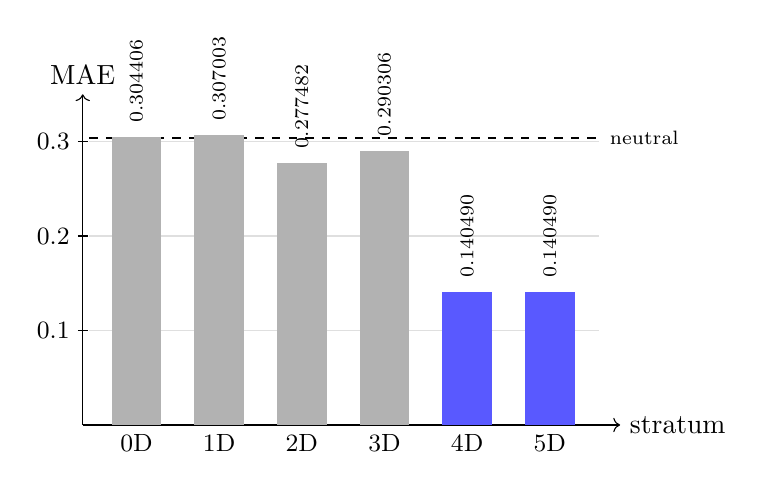
\begin{tikzpicture}[x=1.05cm,y=12cm]
  \draw[->] (0,0) -- (6.5,0) node[right] {stratum};
  \draw[->] (0,0) -- (0,0.35) node[above] {MAE};
  \foreach \y in {0.1,0.2,0.3}{
    \draw (-0.06,\y) -- (0.06,\y) node[left=3pt] {\small \y};
    \draw[gray!25] (0.08,\y) -- (6.25,\y);
  }
  \draw[dashed,thick] (0.08,0.303944) -- (6.25,0.303944)
    node[right] {\scriptsize neutral};
  \foreach \x/\h/\lab in {
    0.65/0.304406/0D,
    1.65/0.307003/1D,
    2.65/0.277482/2D,
    3.65/0.290306/3D}{
    \fill[gray!60] (\x-0.30,0) rectangle (\x+0.30,\h);
    \node[below] at (\x,0) {\small \lab};
    \node[above,rotate=90,anchor=west] at (\x,\h+0.005) {\scriptsize \h};
  }
  \foreach \x/\h/\lab in {4.65/0.140490/4D,5.65/0.140490/5D}{
    \fill[blue!65] (\x-0.30,0) rectangle (\x+0.30,\h);
    \node[below] at (\x,0) {\small \lab};
    \node[above,rotate=90,anchor=west] at (\x,\h+0.005) {\scriptsize \h};
  }
\end{tikzpicture}
\caption{The geometric strata alone remain near the neutral baseline.  The principal held-out
error reduction appears when the normalized prime coordinate is added.}
\label{fig:ablation}
\end{figure}

The zero-dimensional and one-dimensional calculations fail in the precise sense that their
errors are indistinguishable from, or slightly worse than, the neutral predictor.  Geometric
lifting to two and three coordinates changes the representation but does not create monotone
predictive improvement.  The decisive empirical reduction occurs at $4D$, where the arithmetic
prime field is added: the MAE falls by $53.78\%$ relative to the neutral $d=1$ predictor.  Adding
$K$ produces no further change on this data set because every evaluated ordinate was placed on
the critical line and therefore $K=0$.  This equality of the $4D$ and $5D$ rows is a necessary
internal control; it is not a certification that unobserved zeros also have $K=0$.

The ablation therefore establishes an information hierarchy, not RH: $0D$ collapses identity,
$1D$ loses $\beta$, $2D$ can represent the analytic location, $3D$ represents the complex
evolution, $4D$ supplies the observed prime-sensitive localization signal, and $5D$ exposes
hypothetical transverse displacement through $K$.  Universal critical-line certification still
requires an arithmetic argument applying to the full zero set rather than only to the tabulated
critical-line ordinates.

\subsection{Ternary Planck hierarchy and residual phase}\label{subsec:ternary}
We now record a separate scale hypothesis suggested by the three spatial coordinates used in the
geometric representation.  The choice of the integer $3$ is motivated by these three spatial
dimensions: the proposed model asks whether an isotropic three-channel organization leaves a
preferred discrete scale ratio equal to $3$.  This motivation does \emph{not} constitute a
derivation.  The existence of three independent spatial coordinates does not, by itself, imply
that every physical length must transform as $L\mapsto3L$.  Accordingly, everything in this
subsection is kept logically independent of the RH implications above.  The relevant mathematical
background is discrete scale invariance, for which a preferred ratio is an additional property of
the system rather than a consequence of ordinary dimensional analysis
\cite{SornetteDSI,Calcagni2017}.

Let $\ell_P$ denote the Planck length.  Using the 2022 CODATA value
\cite{CODATA2022},
\begin{equation}\label{eq:planck-length}
  \ell_P=1.616255(18)\times10^{-35}\ {\rm m},
\end{equation}
define the exact ternary sequence
\begin{equation}\label{eq:ternary-sequence}
  L_n=\ell_P3^n,\qquad n\in\mathbb Z.
\end{equation}
For the finite progression $0\le n\le129$,
\begin{equation}
  \resizebox{0.96\linewidth}{!}{$
  3^{129}=35370553733215749514562618584237555997034634776827523327290883$}
\end{equation}
and hence
\begin{equation}\label{eq:L129}
  L_{129}=5.716783432407862\times10^{26}\ {\rm m}.
\end{equation}
A representative present-day comoving radius of the observable Universe is approximately
$R_{\rm obs}=4.40\times10^{26}\,{\rm m}$, or about $46.5$ billion light-years, within the
standard cosmological picture \cite{Planck2018,NASACosmicTimes}.  Consequently,
\begin{equation}
  L_{128}=1.905594477469287\times10^{26}\,{\rm m}
  <R_{\rm obs}<L_{129},\qquad
  \frac{L_{129}}{R_{\rm obs}}\simeq1.2993.
\end{equation}
This bracketing is a numerical observation, not evidence by itself that cosmological scales are
quantized in powers of $3$.

For any positive measured scale $L_i$, define its base-$3$ coordinate, nearest stratum, and
residual by
\begin{equation}\label{eq:ternary-residual}
  q_i=\log_3\!\left(\frac{L_i}{\ell_P}\right),\qquad
  n_i=\operatorname{round}(q_i),\qquad
  \delta_i=q_i-n_i\in[-\tfrac12,\tfrac12].
\end{equation}
This is an exact change of coordinates:
\begin{equation}\label{eq:ternary-reconstruction}
  L_i=\ell_P3^{n_i+\delta_i}=L_{n_i}3^{\delta_i}.
\end{equation}
Thus $n_i$ labels a discrete scale stratum, while $\delta_i$ records the within-stratum location.
It is useful to call $\theta_i=2\pi\delta_i$ a logarithmic phase.  A nonzero residual is not
automatically an error: a family-dependent version may be written
\begin{equation}\label{eq:ternary-families}
  L_{n,a}=\ell_P3^{n+\delta_a},
\end{equation}
where $a$ labels a consistently defined physical family and $\delta_a$ is a phase offset to be
estimated from data.  The boundary $|\delta_i|=1/2$ merely means that $L_i$ is logarithmically
equidistant from two adjacent ternary levels.  It has no mathematical identity with the critical
line $\Re(s)=1/2$.

The residual also supplies a controlled local expansion.  Since
\begin{equation}
  3^\delta=e^{(\log3)\delta}
  =\sum_{k=0}^{\infty}\frac{[(\log3)\delta]^k}{k!},
\end{equation}
equation~\eqref{eq:ternary-reconstruction} becomes
\begin{equation}\label{eq:ternary-taylor}
  L_i=L_{n_i}\left[1+(\log3)\delta_i
  +\frac{(\log3)^2}{2}\delta_i^2
  +\frac{(\log3)^3}{6}\delta_i^3+\cdots\right].
\end{equation}
The first coefficients are $1.0986122887$, $0.603474$, $0.221014$, $0.060701$, and
$0.013337$.  Even at the endpoint $\delta=1/2$, truncation after the sixth power approximates
$\sqrt3$ with relative error $-1.86\times10^{-6}$.

An exploratory calculation on 14 heterogeneous reference scales gave
\begin{equation}
  \overline\delta=0.236231,\qquad
  \overline{|\delta|}=0.314932,\qquad
  \max|\delta|=0.452459.
\end{equation}
For a uniform null distribution on $[-1/2,1/2]$, one has
$\mathbb E|\delta|=1/4$.  The illustrative sample therefore does \emph{not} show concentration
around zero.  Moreover, it was not preregistered and mixes radii, widths, heights, and distances;
changing radius to diameter shifts the phase by $\log_3 2$ modulo one.  A legitimate test must
predefine homogeneous observables, measurement uncertainties, selection rules, the null model,
and a held-out replication set.  The present result is therefore a reproducible coordinate system
and a test protocol, not an established law fixing the sizes of planets, particles, or the
Universe.  Such bounds also depend on dynamics, gravity, interactions, and equations of state.

\subsection{From a scale code to a dynamical unification criterion}\label{subsec:unification}
If the ternary organization survives prospective tests, equation~\eqref{eq:ternary-families}
provides a common \emph{kinematic} code for quantum, macroscopic, and cosmological scales.  This
possibility is anchored at
\begin{equation}\label{eq:planck-bridge}
  \ell_P=\sqrt{\frac{\hbar G}{c^3}},
\end{equation}
which already combines the quantum constant $\hbar$, the gravitational constant $G$, and the
relativistic invariant speed $c$.  A shared scale coordinate is not yet a dynamical unification,
however.  That stronger claim requires a single evolution law whose controlled limits reproduce
quantum theory and general relativity.

For this purpose define the inverse scale
\begin{equation}\label{eq:ternary-mu}
  \mu_{n,a}=L_{n,a}^{-1}=\ell_P^{-1}3^{-(n+\delta_a)},
  \qquad \mu_{n+1,a}=\frac{\mu_{n,a}}{3}.
\end{equation}
The passage $n\mapsto n+1$ is then a finite coarse-graining step.  This interpretation is
compatible with the renormalization-group idea that effective couplings and fields depend on the
resolution scale, including scale-dependent effective actions used in quantum-gravity research
\cite{Reuter1998,Donoghue1994,Ambjorn2024}.  It does not require the continuum flow to be
fundamentally discrete; the ternary model instead proposes that physically distinguished sections
of that flow occur at the scales~\eqref{eq:ternary-mu}.

Introduce a state at each stratum,
\begin{equation}\label{eq:cross-scale-state}
  \mathcal S_{n,a}
  =\bigl(n,\delta_a,\Psi_{n,a},g^{(n,a)}_{\mu\nu},\mathbf g_{n,a}\bigr),
\end{equation}
where $\Psi_{n,a}$ denotes the quantum state or matter fields,
$g^{(n,a)}_{\mu\nu}$ the effective spacetime metric, and $\mathbf g_{n,a}$ the dimensionless
couplings.  The missing dynamical object is a transition operator
\begin{equation}\label{eq:cross-scale-transition}
  \mathcal T_{n,a}:\mathcal S_{n,a}\longmapsto\mathcal S_{n+1,a},
  \qquad
  \mathcal T^{(m)}_{n,a}
  =\mathcal T_{n+m-1,a}\circ\cdots\circ\mathcal T_{n,a}.
\end{equation}
The phase need not remain fixed: interactions or a change of physical family may produce
$\delta_a\mapsto\delta'_a$.  Equation~\eqref{eq:cross-scale-transition} therefore supplies the
precise location at which the proposed amplitude--phase variables, conservation laws, and
dimensionless Buckingham groups must enter.

\paragraph{Worked one-step example.}
To demonstrate how a calculable transition would operate, let one component $g_n$ of
$\mathbf g_{n,a}$ obey the toy one-loop flow
\begin{equation}\label{eq:toy-beta}
  \frac{dg}{d\log\mu}=b g^2.
\end{equation}
Because $\log\mu_{n+1}-\log\mu_n=-\log3$, exact integration over one ternary step gives
\begin{equation}\label{eq:toy-step}
  \frac{1}{g_{n+1}}=\frac{1}{g_n}+b\log3.
\end{equation}
For $g_n=0.2000$ and $b=0.1000$,
\begin{equation}
  g_{n+1}=\frac{1}{5+0.1\log3}=0.19570\ldots .
\end{equation}
The algebraic inverse,
\begin{equation}
  \frac{1}{g_n}=\frac{1}{g_{n+1}}-b\log3,
\end{equation}
recovers the initial coupling whenever the denominator is nonzero.  This example makes a next
state numerically definite once a beta function and initial data are supplied.  It does not prove
that the chosen beta function describes Nature, and algebraic reversibility of the coupling does
not restore microscopic degrees of freedom that a genuine coarse-graining operation may have
integrated out.

\paragraph{Spherical reduction from three spatial coordinates to one.}
The monopole breathing construction gives a second, geometrically exact example.  Expand a scalar
degree of freedom in spherical harmonics,
\begin{equation}\label{eq:spherical-expansion}
  \Phi(t,r,\vartheta,\varphi)
  =\sum_{\ell=0}^{\infty}\sum_{m=-\ell}^{\ell}
  \phi_{\ell m}(t,r)Y_{\ell m}(\vartheta,\varphi).
\end{equation}
Spherical symmetry selects the monopole sector $\ell=m=0$, so that
\begin{equation}\label{eq:monopole-reduction}
  \Phi(t,r,\vartheta,\varphi)
  =\phi_{00}(t,r)Y_{00}
  =\frac{\phi_0(t,r)}{\sqrt{4\pi}}.
\end{equation}
The angular coordinates have not been assigned arbitrary values; their dependence is fixed by the
unique constant harmonic $Y_{00}$.  For a static spherically symmetric line element
\begin{equation}
  ds^2=-f(r)c^2dt^2+f(r)^{-1}dr^2+r^2d\Omega^2,
\end{equation}
the angular integral in the scalar action can then be performed exactly.  With the harmonic
normalized by $\int|Y_{00}|^2d\Omega=1$, one obtains, up to the chosen field normalization,
\begin{equation}\label{eq:radial-action}
  S_0=-\frac12\int dt\,dr\,r^2
  \left[-\frac{1}{f(r)c^2}(\partial_t\phi_0)^2
  +f(r)(\partial_r\phi_0)^2\right].
\end{equation}
Thus a $3+1$-dimensional field problem reduces to an effective $1+1$-dimensional problem
$(t,r)$; on a fixed-time spatial slice only the radial coordinate remains.  This is the precise
mathematical sense in which the monopole model passes from three spatial coordinates to one.
The reduced action is also a concrete interface between a quantum field mode $\phi_0$ and a
relativistic geometry $f(r)$.  It becomes a fundamental unification only if the geometry and its
backreaction are themselves included in the quantum dynamics rather than held fixed as a
classical background.
The minimal semiclassical closure promotes the spherical factor to $f(t,r)$ and couples the
geometry to the quantum expectation value of stress--energy,
\begin{equation}\label{eq:semiclassical-backreaction}
  G_{\mu\nu}[g]+\Lambda g_{\mu\nu}
  =\frac{8\pi G}{c^4}
  \langle\Psi|\widehat T_{\mu\nu}[\phi_0,g]|\Psi\rangle .
\end{equation}
Equation~\eqref{eq:semiclassical-backreaction} supplies the missing feedback variable: the field
changes the geometry and the geometry changes the field evolution.  It is a semiclassical
interface, not yet a quantization of $g_{\mu\nu}$ itself \cite{BirrellDavies}.

Black-hole horizon encoding is related but dimensionally different.  The Bekenstein--Hawking
entropy is proportional to the two-dimensional horizon area,
\begin{equation}\label{eq:bh-entropy}
  S_{\rm BH}=\frac{k_Bc^3A}{4G\hbar}=\frac{k_BA}{4\ell_P^2},
\end{equation}
which motivated holographic descriptions of bulk information
\cite{Bekenstein1973,Hawking1975,Susskind1995}.  Equation~\eqref{eq:radial-action} is an exact
symmetry reduction, whereas equation~\eqref{eq:bh-entropy} is an area law.  Neither identity alone
proves unitary recovery of all information from a completely evaporating black hole.  Modern
replica-wormhole and island calculations address that further dynamical question
\cite{Almheiri2020}; it must not be inserted as a consequence of spherical symmetry.

\paragraph{Entropy as an evidential observable.}
The proposed transition can be tested through an entropy budget.  For a reduced quantum state
$\widehat\rho_{n,a}$, define
\begin{equation}\label{eq:von-neumann-stratum}
  S_{\rm vN}(n,a)=-k_B\operatorname{Tr}
  \bigl(\widehat\rho_{n,a}\log\widehat\rho_{n,a}\bigr).
\end{equation}
For a black-hole sector, the appropriate quantity is the generalized entropy
\begin{equation}\label{eq:generalized-entropy}
  S_{\rm gen}(n)=\frac{k_BA_n}{4\ell_P^2}+S_{\rm out}(n),
\end{equation}
combining horizon area with the entropy of quantum fields outside the horizon.  A ternary
transition makes the definite comparison
\begin{equation}\label{eq:entropy-step}
  \Delta_3S_{\rm gen}(n)
  =S_{\rm gen}(n+1)-S_{\rm gen}(n),
  \qquad \mu_{n+1}=\mu_n/3.
\end{equation}
Under the hypotheses of the generalized second law, the expected sign is
$\Delta_3S_{\rm gen}\ge0$ \cite{Wall2012}.  For a fundamentally closed unitary system, however,
the entropy of the complete state remains constant; an increase in a reduced entropy represents
entanglement or coarse graining, not destruction of total information.  The associated mutual
information,
\begin{equation}\label{eq:mutual-information-link}
  I(\text{field}:\text{geometry})
  =S_{\rm field}+S_{\rm geometry}-S_{\rm total}\ge0,
\end{equation}
measures correlations stored across the two sectors.

Evidence for the model would therefore require the same frozen transition rule to predict the
magnitude, not only the sign, of~\eqref{eq:entropy-step} over several strata.  The comparison must
include continuous-scale evolution and alternative discrete ratios as null competitors.  A
smaller held-out error for ratio $3$, together with conservation of total information and the
predicted redistribution between area, exterior fields, and mutual information, would support
the ternary dynamics.  Entropy measurements alone, without this quantitative competitor test,
would not identify the base $3$ uniquely.

A candidate action realizing this program may be organized schematically as
\begin{equation}\label{eq:cross-scale-action}
  \begin{aligned}
  S&=\sum_{n,a}\int d^4x\,\sqrt{-g^{(n,a)}}\,\mathcal L_{n,a},\\
  \mathcal L_{n,a}
  &=\frac{c^3}{16\pi G_{n,a}}\bigl(R_{n,a}-2\Lambda_{n,a}\bigr)\\
  &\quad+\mathcal L_{\rm matter}(\Psi_{n,a},g^{(n,a)};\mathbf g_{n,a})\\
  &\quad+\mathcal L_{\rm link}(\mathcal S_{n,a},\mathcal S_{n+1,a}).
  \end{aligned}
\end{equation}
Here $\mathcal L_{\rm link}$ is not supplied by the scale identity and must be derived or fitted
without using the observations later claimed as predictions.  It encodes the transport of
information between adjacent strata and distinguishes a physical theory from a relabeling of
lengths.

We therefore define a \emph{dynamical ternary unification} only if the same specified model
satisfies all of the following tests:
\begin{enumerate}[label=(U\arabic*)]
  \item \textbf{Closure:} the maps $\mathcal T_{n,a}$ are well defined and their compositions do
  not depend on an unstated change of variables or units.
  \item \textbf{Quantum:} microscopic evolution preserves probabilities---unitarily
  for closed systems, or by a completely positive, trace-preserving map when open.
  \item \textbf{Relativistic consistency:} the macroscopic equations are generally covariant and
  recover Einstein dynamics, with controlled corrections, in the appropriate limit.
  \item \textbf{Conservation:} symmetries of~\eqref{eq:cross-scale-action} generate the associated
  Noether conservation laws; apparent loss in one stratum is balanced by the link and neighboring
  strata rather than deleted by definition.
  \item \textbf{Correspondence:} the same parameters recover tested quantum-field behavior at
  short distances and tested gravitational behavior at long distances.
  \item \textbf{Prediction:} parameters calibrated on a frozen training set predict held-out
  scales, transition phases, or dimensionless observables more accurately than continuous-scale
  and alternative-base models.
\end{enumerate}
Meeting these conditions would promote the ternary hierarchy from a coordinate system to a
candidate unifying dynamics.  At present, equations~\eqref{eq:cross-scale-state}--
\eqref{eq:cross-scale-action} specify the deductive research program and expose its missing term:
the independently justified link dynamics $\mathcal L_{\rm link}$.  They do not yet establish
that Nature selects the ratio $3$ or that quantum gravity has been derived.

\section{Conclusions}
The revised framework is ordered in linked but logically separated levels:
\begin{equation}
 \boxed{\begin{gathered}
 \text{analytic identity}\to F_2/F_4\to\text{graph involution},\\
 [L,P_R]=0\to[J_c,J_n]=0\to(P_{\parallel},P_{\perp},O_2),\\
 \text{asymptotic wave}\to K\to\text{finite-height confinement criterion},\\
 \text{prime field}\to\text{passive spectral target}\to\text{held-out tests}.
 \end{gathered}}
\end{equation}
The ternary Planck construction of Section~\ref{subsec:ternary} is likewise kept separate: it is
a falsifiable discrete-scale ansatz motivated by the model's three spatial coordinates, and it is
not used in any proof or conditional confinement statement concerning the critical line.
Section~\ref{subsec:unification} identifies the exact monopolar $3D\to1D$ reduction, the
field--geometry backreaction variable, and an entropy-based validation protocol.  These provide a
defined quantum--relativistic interface; promotion to a fundamental unification requires an
independently derived link dynamics and successful held-out predictions.
The critical reversible closure is established by the identity
\begin{equation}
 1-\rho=\bar\rho\iff\Re(\rho)=1/2.
\end{equation}
The symmetry graph turns this identity into an orbit reduction from four to two positions. The null--neutral--non-null pipeline permits the multiscale topology of the ordinates to be studied separately through $H_0$. Voros's secondary functions provide an established precedent for speaking of a second generation built over the zeros.  The M\"obius coordinate adds a complementary exact description: reflection preserves phase and reciprocates amplitude.  Buckingham reduction then isolates $K=(\beta-1/2)/\gamma$ as the dimensionless transverse deformation.

The asymptotic-wave mechanism makes the two scalar axes explicit.  Critical reflection is
$J_c=\operatorname{diag}(-1,1)$, so $P_{\perp}$ detects the sole confinement defect and
$P_{\parallel}$ preserves the ordinate.  Nodal inversion is instead $J_n=-I_2$, for which
$I_2+J_n=O_2$ has rank zero.  The commutation law shows that these decompositions are
compatible with the graph symmetry sectors.  Theorem~\ref{thm:injective-confinement} then
states the finite-$T$ closure exactly: an injective cell representation commuting with the
critical reflection has no $F_4$ sector, and verification for every finite $T$ gives the
universal critical-line statement.

The paired Smith construction in Section~\ref{subsec:quaternion-smith} gives a further exact
representation of the same reflection.  The lift
$Q_\rho=w(\rho)+w(R\rho)j$ embeds the direct and reflected complex coordinates in
$\mathbb H$, and the component exchange $\mathcal P$ satisfies
$\Phi\circ R=\mathcal P\circ\Phi$.  Consequently its nonnegative defect
$\mathcal D_{\mathbb H}(\rho)$ vanishes exactly on the critical line.  After separating
$Q_\rho=r_\rho U_\rho$, the scale is retained by $r_\rho$ and the unit orientation lies on
$S^3$.  The associated two complex coordinates are reflection-linked, so this is an exact
two-dimensional embedding in four real coordinates rather than a claim that the zero set
fills the whole hypersphere.

The prime-channel construction in Proposition~\ref{prop:prime-defect-unique-intersection}
retains the same reflected orientation with an explicit $\pm$ square-root pair.  Its squared
separation is a positive sum of $\sinh^2$ terms, so phase cancellation cannot hide a transverse
component.  The global quantity $\mathfrak G_{P,M}(T)$ sums these squared defects over the
complete analytic zero set with multiplicity, and Theorem~\ref{thm:global-summed-prime-defect}
shows that its nullity is exactly equivalent to the absence of the $F_4$ sector below $T$.
The algebraic cancellation of the two signed branches is kept distinct from this positive
summed-defect criterion.

Section~\ref{sec:cantor-closure} completes the coordinate and set-theoretic organization.
Every zero position defines one occupied node as the intersection of its two coordinate lines.
The inside--outside and above--below involutions generate a four-node Klein orbit whose average
is the null vector; this cancellation centers the orbit but does not replace individual
fixedness.  Unit-cell uniqueness converts reflection invariance into fixedness.  Cantor pairing
then flattens the integer cell grid to one reversible discrete address, while the exact
prime-power identity \eqref{eq:prime-power-line} supplies the arithmetic content of the
one-dimensional signal.  Finally, the nested-cubical lemma separates a finite numerical bound
from exact confinement: transverse widths tending to zero force $x=0$ only when membership is
established at every stage.  Buckingham reduction remains compatible with this construction by
providing dimensionless state invariants rather than a second cell enumeration.

The methodological contribution of the present text is to integrate these pieces into a reproducible scheme with explicit scope conditions. Theorem~\ref{thm:commutation-law} is the matrix and graph compatibility law; Theorem~\ref{thm:injective-confinement} is the finite-height cell criterion; Theorem~\ref{thm:saturation} is a set-theoretic saturation criterion; Theorem~\ref{thm:cycle-passivity} is a conditional dynamical confinement theorem; and \eqref{eq:predictMAE} is a finite out-of-sample result.  None is substituted for another.  The operator route becomes decisive only if its characteristic function is derived arithmetically and shown to reproduce $\xi$ without assuming the location of its zeros.  The empirical route remains falsifiable through frozen replication at larger heights.  This separation preserves the exact content of the symmetry, commutation, matrix-compression, and passivity results while identifying the concrete analytic construction on which a full spectral conclusion depends.

The Euler--Fourier extension in Section~\ref{sec:euler-fourier-drum} now supplies the missing
prime--singularity bridge in operational form.  The identities
\eqref{eq:eulerTraceZeta}--\eqref{eq:primeSelector} prove that the arithmetic drum resolves
each prime-power channel uniquely, while the finite sonifications and graphical audit expose
that reconstruction directly.  The universal logical closure is Theorem
\ref{thm:universal-route-equivalence}: RH, reality of every $E_\rho$, nullity of
$\mathcal P_{\rm ext}(T)$ at every finite height, and nullity of the positive prime defect are
equivalent statements.  Corollary~\ref{cor:spectral-completion-target} fixes the sole
operator-theoretic completion target.  Thus the manuscript closes the arithmetic bridge and
the exact reduction without replacing the still-independent determinant realization by a
finite computation or an acoustic analogy.

The relativistic extension fixes the previously free playback scale by
$\kappa=c/L_0$.  It converts the same $m\log p$ channels into massless dispersion modes,
constructs their balanced standing-wave superposition, and identifies the commuting
arithmetic angular momenta $\widehat L_p=\hbar N_p$.  Equation
\eqref{eq:passiveNormBalance} separates conservative propagation from passive loss, while
\eqref{eq:primeInteractionTarget} states the precise interaction problem that connects the
free prime spectrum to the completed-zero spectrum.  The accompanying numerical audit tests
the wave discretization and is retained as reproducible support rather than as a substitute
for the analytic determinant identity.

\appendix
\section{Pseudocode for the non-null graph}
\begin{verbatim}
input: gamma[1..N], epsilon_grid
x[n] = Nbar(gamma[n])

for epsilon in epsilon_grid:
    A = zeros(N,N)
    for i < j:
        if abs(x[i]-x[j]) <= epsilon:
            A[i,j] = A[j,i] = 1
    D = diag(row_sums(A))
    L = D - A
    eigenvalues = eigvalsh(L)
    beta0 = count(abs(eigenvalues) < tolerance)
    save(epsilon, beta0, eigenvalues)
\end{verbatim}

\section{Pseudocode for the family identifier}
\begin{verbatim}
input: rho
C = conjugate(rho)
F = 1 - rho
R = 1 - conjugate(rho)
Delta = F - C

orbit = unique({rho, C, F, R})
if R == rho:
    family = F2
else:
    family = F4
\end{verbatim}

\section{Operator extension: radial monopole, breathing mode, and spectrum}\label{sec:monopolo}
\subsection{Two meanings of ``monopole''}
In this work the term \emph{monopole operator} is used in the nuclear sense of multipolarity $L=0$. It must not be confused with the Dirac magnetic monopole, which would correspond to a hypothetical isolated magnetic charge. The distinction is relevant: the former is an established collective operator in nuclear physics; the latter is a hypothetical particle sought experimentally.

\subsection{Isoscalar monopole operator}
For a nucleus of mass number $A$, the one-body isoscalar monopole operator is represented by the quadratic radial coordinate and, at the many-body level, by
\begin{equation}\label{eq:mis0}
  \widehat M_{\rm IS0}=\sum_{i=1}^{A} r_i^2 .
\end{equation}
It is a scalar operator under rotations and selects monopole excitations $J^\pi=0^+$. The associated strength function can be written as
\begin{equation}\label{eq:monostrength}
 S_{\rm IS0}(E)=\sum_{\nu}
 \left|\langle \Psi_\nu|\widehat M_{\rm IS0}|\Psi_0\rangle\right|^2
 \delta\!\left(E-(E_\nu-E_0)\right).
\end{equation}
The isoscalar giant monopole resonance (ISGMR) corresponds to a collective radial response in which protons and neutrons oscillate approximately in phase. It is therefore called a \emph{breathing mode}: the nuclear distribution moves between configurations of higher and lower density while preserving, to first approximation, spherical symmetry.

For electric monopole $E0$ transitions, the charge operator contains the proton analogue
\begin{equation}\label{eq:e0op}
  \widehat M(E0)=e\sum_{p=1}^{Z} r_p^2,
\end{equation}
and the transition strength is determined by its matrix element. In a pure $E0$ transition, single-photon emission is forbidden by angular-momentum conservation; the channels include internal conversion and, when energetically allowed, internal $e^-e^+$ pair creation.

\subsection{Collective coordinate and maximum--minimum}
The geometry of the mode can be idealized through a collective radial coordinate
\begin{equation}\label{eq:radialcollective}
  R_c(t)=R_0+A_M\cos(\omega_M t+\phi),
\end{equation}
with
\begin{equation}
  R_{\max}=R_0+A_M,
  \qquad
  R_{\min}=R_0-A_M.
\end{equation}
The centered variable
\begin{equation}
  x(t)=R_c(t)-R_0
\end{equation}
has the radial involution
\begin{equation}\label{eq:radialinvolution}
  \mathcal J:x\mapsto -x,
  \qquad
  \mathcal J^2=I.
\end{equation}
Thus expansion and compression appear as homologous states relative to the fixed point $x=0$, representing the equilibrium radius. The extrema $+A_M$ and $-A_M$ form a pair under $\mathcal J$.

\subsection{Collective Hamiltonian and quantization}
Near equilibrium, the harmonic approximation leads to the collective Hamiltonian
\begin{equation}\label{eq:monoham}
 H_M=\frac{P_c^2}{2M_{\rm eff}}
     +\frac12 C_M(R_c-R_0)^2,
 \qquad
 \omega_M=\sqrt{\frac{C_M}{M_{\rm eff}}},
\end{equation}
where $M_{\rm eff}$ is the collective inertia and $C_M$ the restoring stiffness. Hamilton's equations imply
\begin{equation}
  \ddot R_c+\omega_M^2(R_c-R_0)=0,
\end{equation}
which recovers \eqref{eq:radialcollective}. Quantizing the radial coordinate gives
\begin{equation}\label{eq:monohamq}
 \widehat H_M=
 -\frac{\hbar^2}{2M_{\rm eff}}\frac{d^2}{dR_c^2}
 +\frac12 C_M(R_c-R_0)^2,
\end{equation}
and, in the ideal harmonic approximation,
\begin{equation}
 E_n=\hbar\omega_M\left(n+\frac12\right).
\end{equation}
The resonance frequency determines the scale at which the monopole response is maximized; the observed spectral width encodes damping and fragmentation of the collective mode.

\subsection{Structural correspondence with the graph-operator language}
The nuclear monopole operator $\widehat M_{\rm IS0}$ and the graph symmetry operator $P_R$ belong to different theories, but they permit comparison of the same abstract architecture:
\begin{equation}\label{eq:operatorparallel}
\begin{array}{ccc}
\text{radial mode} &:& \mathcal J^2=I,\quad x\leftrightarrow -x,\quad \operatorname{Fix}(\mathcal J)=\{0\},\\[1mm]
\text{Riemann graph} &:& P_R^2=I,\quad v_\rho\leftrightarrow v_{R(\rho)},\quad \operatorname{Fix}(P_R).
\end{array}
\end{equation}
In both cases there is an involution, a fixed set, and a decomposition of the space into sectors even and odd with respect to the operator. If the operator commutes with the corresponding spectral generator, their eigenspaces can be organized simultaneously. For the graph, this condition is
\begin{equation}
 [L,P_R]=0.
\end{equation}
For the ideal monopole oscillator, the radial reflection $\mathcal J$ commutes with the harmonic Hamiltonian,
\begin{equation}\label{eq:monoparity}
 [\widehat H_M,\mathcal J]=0,
\end{equation}
because the potential depends on $(R_c-R_0)^2$. Thus both languages explicitly exhibit an involutive symmetry compatible with a spectral operator.

This correspondence does not physically identify $P_R$ with $\widehat M_{\rm IS0}$ or $\widehat H_M$; it establishes an equivalence of operator architecture: involution, fixed point, homologous pairs, commutation with a spectral operator, and organization of eigenmodes. This parallelism provides a common language for describing the maximum--minimum closure of the monopole mode and the closure of orbits under $R(s)=1-\overline{s}$.

\section{Passive--adjoint criterion and conservation of realizability}

\subsection{Two reflections and the centered variable}
The holomorphic functional reflection $F(s)=1-s$ and the same-height critical reflection
$R(s)=1-\overline s$ must be distinguished.  For $z=s-1/2$ they act as
\begin{equation}
 F:z\mapsto-z,
 \qquad
 R:z\mapsto-\overline z.
\end{equation}
The second action is the one implemented by an adjoint-reflection architecture.

\subsection{Horizontal energy coordinate and the Hardy amplitude}
The centered spectral coordinate becomes a real-energy coordinate after a quarter-turn of
the complex plane.

\begin{proposition}[Exact energy-axis rotation]\label{prop:energy-axis-rotation}
Let
\begin{equation}\label{eq:energyrotation}
 s=\beta+i\gamma,
 \qquad z=s-\frac12,
 \qquad E=-iz.
\end{equation}
Then
\begin{equation}\label{eq:energycomponents}
 E=\gamma-i\left(\beta-\frac12\right),
 \qquad \Re E=\gamma,
 \qquad \Im E=-\left(\beta-\frac12\right),
\end{equation}
and hence
\begin{equation}\label{eq:energyaxis-equivalence}
 \Re s=\frac12
 \quad\Longleftrightarrow\quad
 z\in i\mathbb R
 \quad\Longleftrightarrow\quad
 E\in\mathbb R.
\end{equation}
For real $E$, define the Riemann--Siegel phase and Hardy function by
\begin{equation}\label{eq:hardyZ}
 \vartheta(E)=\Im\log\Gamma\!\left(\frac14+\frac{iE}{2}\right)
               -\frac{E}{2}\log\pi,
 \qquad
 Z(E)=e^{i\vartheta(E)}\zeta\!\left(\frac12+iE\right).
\end{equation}
Then $Z(E)$ is real-valued and
\begin{equation}\label{eq:hardyzeros}
 Z(E)=0
 \quad\Longleftrightarrow\quad
 \zeta\!\left(\frac12+iE\right)=0.
\end{equation}
If $H=H^*$ is a quantum Hamiltonian and $A=iH$, then
\begin{equation}\label{eq:energygenerator}
 A^*=-A,
 \qquad \sigma(A)=i\sigma(H)\subset i\mathbb R.
\end{equation}
Thus a real energy $E_n\in\sigma(H)$ is carried to the centered spectral value
$z_n=iE_n$.  The alternative convention $A=-iH$ carries $E_n$ to the reflected value
$-iE_n$.
\end{proposition}

\begin{proof}
Substitution in \eqref{eq:energyrotation} gives
\[
 E=-i\left[\left(\beta-\frac12\right)+i\gamma\right]
   =\gamma-i\left(\beta-\frac12\right),
\]
which proves \eqref{eq:energycomponents}--\eqref{eq:energyaxis-equivalence}.  For real $E$,
complex conjugation gives
$\overline{\zeta(1/2+iE)}=\zeta(1/2-iE)$.  On the critical line, the functional-equation
factor satisfies
\begin{equation}\label{eq:chi-theta}
 \chi\!\left(\frac12+iE\right)=e^{-2i\vartheta(E)},
 \qquad
 \zeta\!\left(\frac12+iE\right)
 =\chi\!\left(\frac12+iE\right)\zeta\!\left(\frac12-iE\right).
\end{equation}
Consequently,
\[
 \overline{Z(E)}
 =e^{-i\vartheta(E)}\zeta\!\left(\frac12-iE\right)
 =e^{i\vartheta(E)}\zeta\!\left(\frac12+iE\right)
 =Z(E),
\]
so $Z(E)\in\mathbb R$.  Since the phase factor never vanishes,
\eqref{eq:hardyzeros} follows.  Finally, $H=H^*$ gives
$(iH)^*=-iH=-A$ and the spectral mapping
$\sigma(iH)=i\sigma(H)$, proving \eqref{eq:energygenerator}.
\end{proof}

\begin{remark}[Scope of the horizontal plot]\label{rem:hardy-scope}
The graph of $Z(E)$ displays exactly the zeros already lying on the critical line, with
horizontal coordinate $E=\gamma$ and vertical amplitude $Z(E)$.  By itself it does not
exclude zeros with $\Im E\ne0$, equivalently $\Re s\ne1/2$.  That exclusion requires the
global spectral realization stated in Theorem~\ref{thm:general-passive-adjoint}.
\end{remark}

\subsection{Abstract spectral criterion}
Let $A$ be a closed, densely defined generator of a strongly continuous contraction semigroup
on a complex Hilbert space $\mathcal H$, and let $J$ be a unitary involution satisfying the
domain-level identity
\begin{equation}\label{eq:JAJ}
 JAJ^{-1}=-A^*.
\end{equation}
The semigroup statements below use the Lumer--Phillips framework and standard Hilbert-space
semigroup theory \cite{LumerPhillips,EngelNagel}.
Since $\sigma(A^*)=\overline{\sigma(A)}$, unitary equivalence gives
\begin{equation}
 \sigma(A)=-\overline{\sigma(A)}.
\end{equation}
Contractivity places $\sigma(A)$ in the closed left half-plane, while the reflected symmetry
places it in the closed right half-plane.  Therefore
\begin{equation}\label{eq:imaginaryspectrum}
 \sigma(A)\subset i\mathbb R.
\end{equation}
Consequently, if an independently constructed arithmetic characteristic function realizes
every nontrivial zero through $z_\rho=\rho-1/2\in\sigma(A)$, then
$\Re\rho=1/2$.

The same hypotheses imply more than spectral confinement.  Conjugating the forward
semigroup by $J$ yields a contractive reverse evolution.  Hence $A$ and $-A$ both generate
contractions, the evolution extends to a unitary group, and
\begin{equation}\label{eq:skewadjoint}
 A^*=-A,
 \qquad [A,J]=0.
\end{equation}
Thus exact reflection plus two-sided passivity collapses dissipation to conservation.

Define the realizable sector by
\begin{equation}
 \mathcal R=\operatorname{Fix}(J)=\{u\in\mathcal H:Ju=u\}.
\end{equation}
Equation \eqref{eq:skewadjoint} implies
\begin{equation}\label{eq:realizability}
 U(t)\mathcal R=\mathcal R,
 \qquad
 \|U(t)u\|=\|u\|.
\end{equation}
We call \eqref{eq:realizability} conservation of realizability: it is a proposed name for the
invariance of an admissible symmetry sector together with norm conservation, not an additional
fundamental law of physics.

\subsection{Open channels and the dilation limitation}
For an effective passive generator
\begin{equation}
 A=-iH_0-\frac12WW^*,
 \qquad H_0=H_0^*,
\end{equation}
one has $A+A^*=-WW^*$.  Exact conservative closure therefore forces $W=0$.  A genuinely
decaying subsystem must consequently be embedded in a larger conservative dilation or treated
through scattering and resonances rather than identified with the final two-sided system.

For the dilation operator
\begin{equation}
 H_0=-i\left(t\frac d{dt}+\frac12\right)
 \quad\text{on }L^2(0,\infty),
\end{equation}
the unitary logarithmic change $(Vf)(x)=e^{x/2}f(e^x)$ transforms $H_0$ into
$-i\,d/dx$ on $L^2(\mathbb R)$.  It has no nonzero square-integrable eigenvectors.  Therefore
critical frequencies in this particular free model must be treated as generalized modes or
resonances, or a different free operator must be constructed; they cannot simply be declared
to be point spectrum.

\section{Mellin--Laplace prime bridge and the spectral target}
Let
\begin{equation}
 \psi(x)=\sum_{n\le x}\Lambda(n),
 \qquad
 \phi_{\Lambda,\varepsilon}(t)
 =e^{-(1/2+\varepsilon)t}\bigl[\psi(e^t)-e^t\bigr].
\end{equation}
With $s=z+1/2+\varepsilon$, the change of variable $x=e^t$ gives, initially for
$\Re s>1$,
\begin{equation}\label{eq:primeLaplace}
 \widehat\phi_{\Lambda,\varepsilon}(z)
 =-\frac1s\frac{\zeta'(s)}{\zeta(s)}-\frac1{s-1}.
\end{equation}
The completed logarithmic derivative is
\begin{equation}\label{eq:xilogderivative}
 \frac{\xi'(s)}{\xi(s)}
 =\frac1s+\frac1{s-1}-\frac12\log\pi
 +\frac12\frac{\Gamma'(s/2)}{\Gamma(s/2)}
 +\frac{\zeta'(s)}{\zeta(s)}.
\end{equation}
Equations \eqref{eq:primeLaplace}--\eqref{eq:xilogderivative} are an exact prime-to-singularity
bridge.  A pole of a transfer function is not automatically an eigenvalue, however, and
membership of $\phi_{\Lambda,\varepsilon}$ in a chosen Hilbert space must be proved rather than
assumed; in the boundary limit it may require a rigged-Hilbert or distributional formulation.

The specific construction to be established is a characteristic or perturbation determinant
\begin{equation}\label{eq:determinanttarget}
 D(z)=E(z)\,\xi\!\left(\frac12+z\right),
 \qquad E(z)\ne0,
\end{equation}
derived from the prime data and compatible with \eqref{eq:JAJ}.

\begin{theorem}[General passive--adjoint arithmetic confinement]\label{thm:general-passive-adjoint}
Let $A$ be a closed, densely defined generator of a strongly continuous contraction
semigroup on a complex Hilbert space $\mathcal H$.  Let $J$ be a unitary involution such that
$J\mathcal D(A)=\mathcal D(A^*)$ and
\begin{equation}\label{eq:generalJAJ}
 JAJ^{-1}=-A^*.
\end{equation}
Then the conclusion
\begin{equation}\label{eq:generalimaginary}
 A^*=-A,
 \qquad \sigma(A)\subset i\mathbb R,
\end{equation}
follows from the operator hypotheses alone and does not assume the Riemann Hypothesis.

Suppose, in addition, that an arithmetic characteristic function $D$ is constructed
independently of RH and satisfies, on a domain containing every shifted nontrivial zero,
\begin{equation}\label{eq:generalrealization}
 D(z)=E(z)\,\xi\!\left(\frac12+z\right),
 \qquad E(z)\ne0,
 \qquad D(z)=0\Longrightarrow z\in\sigma(A).
\end{equation}
Then every nontrivial zero $\rho$ of $\zeta$ satisfies
\begin{equation}\label{eq:generalRHconclusion}
 \rho=\frac12+z_\rho,
 \qquad z_\rho\in i\mathbb R,
 \qquad \Re\rho=\frac12.
\end{equation}
Consequently, once all hypotheses in \eqref{eq:generalJAJ}--\eqref{eq:generalrealization}
have been established without using the location of the zeta zeros, RH is a consequence of
the construction rather than a premise of it.
\end{theorem}

\begin{proof}
Contractivity gives $\sigma(A)\subset\{z:\Re z\le0\}$.  From
\eqref{eq:generalJAJ}, unitary equivalence, and
$\sigma(A^*)=\overline{\sigma(A)}$, one obtains
$\sigma(A)=-\overline{\sigma(A)}$.  Applying the left-half-plane inclusion to the reflected
spectral value forces $\Re z\ge0$ for every $z\in\sigma(A)$; hence
$\sigma(A)\subset i\mathbb R$.  Equivalently, conjugation by $J$ supplies the contractive
reverse evolution.  The forward contraction semigroup therefore extends to a unitary group,
whose generator is skew-adjoint, so $A^*=-A$.

Now let $\rho$ be a nontrivial zero and put $z_\rho=\rho-1/2$.  Since $E$ never vanishes,
\eqref{eq:generalrealization} gives $D(z_\rho)=0$, and the realization hypothesis gives
$z_\rho\in\sigma(A)$.  Equation \eqref{eq:generalimaginary} yields
$\Re z_\rho=0$, whence $\Re\rho=1/2$.
\end{proof}

The theorem separates the independent operator statement from its arithmetic application.
The first paragraph is an unconditional abstract result.  The second becomes an RH proof only
after the determinant, spectral inclusion, and domain identities have themselves been proved
without invoking RH.  Weil positivity and recent operator
realizations of the Weil quadratic form provide the closest established comparison: their
positivity is an RH-equivalent criterion, while their finite-window eigenvalues are auxiliary
variational values and are not automatically the ordinates $\gamma_n$
\cite{ConnesConsaniScaling,ConnesConsaniWeil,Suzuki2026}.

\section{Euler--Fourier arithmetic drum, sonification, and universal routes}
\label{sec:euler-fourier-drum}

This section makes the prime--singularity bridge operational.  The construction has three
separate layers: an exact Euler trace, an exact Fourier decomposition of the logarithmic
derivative, and a finite audible rendering.  The first two are mathematical identities; the
third is a reproducible representation of a finite truncation.

\subsection{Euler Hamiltonian and the prime--integer correspondence}
Let $\mathcal H_E=\ell^2(\mathbb N)$ with canonical basis $\{e_n\}_{n\ge1}$, and define
the nonnegative diagonal operator
\begin{equation}\label{eq:eulerHamiltonian}
 H_Ee_n=(\log n)e_n.
\end{equation}
Unique factorization, $n=\prod_p p^{k_p}$, identifies the same operator with the bosonic
prime-mode sum
\begin{equation}\label{eq:eulerFockHamiltonian}
 H_E=\sum_p(\log p)N_p,
 \qquad
 \log n=\sum_p k_p\log p.
\end{equation}
Consequently, for $\Re s>1$, the trace is absolutely convergent and
\begin{equation}\label{eq:eulerTraceZeta}
 \operatorname{Tr}(e^{-sH_E})
 =\sum_{n\ge1}e^{-s\log n}
 =\sum_{n\ge1}\frac1{n^s}
 =\prod_p\frac1{1-p^{-s}}
 =\zeta(s).
\end{equation}
This is an exact realization of the Euler product as a partition trace.  Logarithmic
differentiation gives the von Mangoldt or prime-power channel expansion
\begin{equation}\label{eq:eulerLogDerivativeComb}
 -\frac{\zeta'(s)}{\zeta(s)}
 =\sum_{n\ge1}\frac{\Lambda(n)}{n^s}
 =\sum_p\sum_{m\ge1}(\log p)p^{-ms},
 \qquad \Re s>1.
\end{equation}
After meromorphic continuation, the logarithmic derivative has a pole at each zero of
$\zeta$, with residue equal to its multiplicity up to the displayed minus sign.  Together
with the elementary pole and gamma terms in \eqref{eq:xilogderivative}, this is the exact
prime--singularity connection used below.

\subsection{Fourier separation and uniqueness of every route}
Fix $\sigma>1$ and set
\begin{equation}\label{eq:primeTimeSignal}
 S_\sigma(t)=-\frac{\zeta'}{\zeta}(\sigma+it)
 =\sum_p\sum_{m\ge1}a_{p,m}(\sigma)e^{-it\omega_{p,m}},
\end{equation}
where
\begin{equation}\label{eq:primeChannelData}
 \omega_{p,m}=m\log p,
 \qquad
 a_{p,m}(\sigma)=(\log p)p^{-m\sigma}.
\end{equation}
Using the Fourier convention
\begin{equation}\label{eq:fourierConvention}
 \widehat f(\omega)=\int_{\mathbb R}f(t)e^{i\omega t}\,dt,
 \qquad
 f(t)=\frac1{2\pi}\int_{\mathbb R}\widehat f(\omega)e^{-i\omega t}\,d\omega,
\end{equation}
the signal is the inverse transform of the distributional comb
\begin{equation}\label{eq:primeFourierComb}
 \widehat S_\sigma(\omega)
 =2\pi\sum_p\sum_{m\ge1}a_{p,m}(\sigma)
 \delta(\omega-m\log p).
\end{equation}

\begin{proposition}[Exact prime-power selector]\label{prop:exact-prime-selector}
For every prime $p$ and integer $m\ge1$,
\begin{equation}\label{eq:primeSelector}
 \mathcal P_{p,m}[S_\sigma]
 :=\lim_{T\to\infty}\frac1{2T}\int_{-T}^{T}
 S_\sigma(t)e^{it m\log p}\,dt
 =(\log p)p^{-m\sigma}.
\end{equation}
Thus every prime-power route is recovered from the complete time signal without ambiguity.
\end{proposition}

\begin{proof}
Absolute convergence for $\sigma>1$ permits termwise averaging.  The mean of
$e^{it(\omega_{p,m}-\omega_{q,n})}$ is zero unless the two frequencies agree.  But
\begin{equation}\label{eq:primeFrequencyUniqueness}
 m\log p=n\log q
 \iff p^m=q^n
 \iff (p,m)=(q,n),
\end{equation}
by unique factorization.  Only the requested coefficient remains.
\end{proof}

Equation \eqref{eq:primeSelector} is the precise meaning of cancellation of the other
channels: it is orthogonal long-time averaging, not deletion of zeta zeros.  Finite $T$
produces a measurable leakage error; the graphical audit displays its decay.

For two channels of equal amplitude in exact phase opposition, the acoustic equilibrium is
\begin{equation}\label{eq:antipodalAcousticCancellation}
 Ae^{i\theta}+Ae^{i(\theta+\pi)}
 =Ae^{i\theta}-Ae^{i\theta}=0.
\end{equation}
Thus a $180^\circ$ phase separation cancels the combined observable.  This signed
cancellation is the acoustic counterpart of the $\pm$ branches already used in the
prime-defect construction.  It is not, by itself, individual nullity: two nonzero terms can
cancel.  The positive quantities $\mathcal P_{\rm ext}(T)$ and
$\mathfrak G_{P,M}(T)$ remove that ambiguity because sums of nonnegative squares vanish only
when every contributing transverse defect vanishes.

\subsection{Finite diagonal drum and exact autocorrelation}
For finite cutoffs $p\le P$ and $1\le m\le M$, let
$\mathcal H_{P,M}=\ell^2\bigl(\{(p,m):p\le P,\ 1\le m\le M\}\bigr)$ and define
\begin{equation}\label{eq:finitePrimeDrum}
 H_{P,M}e_{p,m}=(m\log p)e_{p,m},
 \qquad
 v_{\sigma;p,m}=\sqrt{\log p}\,p^{-m\sigma/2}.
\end{equation}
Then its matrix autocorrelation is exactly the truncated Euler--Fourier signal:
\begin{equation}\label{eq:drumAutocorrelation}
 v_\sigma^*e^{-itH_{P,M}}v_\sigma
 =\sum_{p\le P}\sum_{m=1}^{M}(\log p)p^{-m\sigma}e^{-itm\log p}.
\end{equation}
The accompanying computation uses the first $100$ primes and $M=4$, hence $400$ modes,
at $\sigma=1.1$.  Direct matrix evolution and the right-hand side of
\eqref{eq:drumAutocorrelation} agree to maximum absolute error
\begin{equation}\label{eq:drumNumericalIdentity}
 \max_t\left|v_\sigma^*e^{-itH_{P,M}}v_\sigma
 -\sum_{p\le P}\sum_{m=1}^{M}(\log p)p^{-m\sigma}e^{-itm\log p}\right|
 =1.35\times10^{-16}.
\end{equation}
The audible conversion uses the declared time scale $\kappa=800$,
\begin{equation}\label{eq:audibleScaling}
 f_{p,m}=\frac{\kappa\,m\log p}{2\pi}\ \text{hertz}.
\end{equation}
This scaling changes only playback speed; it does not alter the arithmetic ratios or the
coefficient identity.

\subsection{Relativistic prime wave, angular balance, and passivity}
\label{subsec:relativistic-prime-wave}
Let $L_0>0$ be a reference length and restore physical units with
\begin{equation}\label{eq:relativisticScale}
 \kappa=\frac{c}{L_0}.
\end{equation}
On the arithmetic basis $\{e_n\}$, define the prime-valuation number operators
\begin{equation}\label{eq:primeNumberOperators}
 N_pe_n=v_p(n)e_n,
 \qquad
 \widehat L_p=\hbar N_p,
\end{equation}
where $v_p(n)$ is the exponent of $p$ in $n$.  The physical arithmetic Hamiltonian is
\begin{equation}\label{eq:physicalPrimeHamiltonian}
 \mathsf H_{\rm pr}
 =\frac{\hbar c}{L_0}H_E
 =\frac{c}{L_0}\sum_p(\log p)\widehat L_p.
\end{equation}
Thus
\begin{equation}\label{eq:physicalPrimeEnergy}
 \mathsf H_{\rm pr}e_n
 =\frac{\hbar c}{L_0}(\log n)e_n,
 \qquad
 \operatorname{Tr}\exp\!\left(-\frac{sL_0}{\hbar c}\mathsf H_{\rm pr}\right)
 =\zeta(s),\quad \Re s>1.
\end{equation}
Because all $N_p$ are simultaneously diagonal,
\begin{equation}\label{eq:angularMomentumCommutation}
 [\mathsf H_{\rm pr},\widehat L_p]=0,
 \qquad
 \frac{d}{dt}\langle\widehat L_p\rangle=0
\end{equation}
under the conservative evolution.  The notation $\widehat L_p$ denotes an
\emph{arithmetic angular momentum}: it has the action eigenvalues $m\hbar$ but becomes a
physical orbital or spin angular momentum only after a corresponding rotational degree of
freedom has been specified.

For a prime-power channel $(p,m)$ set
\begin{equation}\label{eq:relativisticPrimeDispersion}
 k_{p,m}=\frac{m\log p}{L_0},
 \qquad
 \omega_{p,m}=ck_{p,m},
 \qquad
 E_{p,m}=\hbar\omega_{p,m}=cP_{p,m}.
\end{equation}
The two equal-amplitude counterpropagating components
\begin{equation}\label{eq:counterpropagatingPrimeBranches}
 \psi_{p,m}^{\pm}(x,t)
 =A_{p,m}e^{\pm ik_{p,m}x-i\omega_{p,m}t}
\end{equation}
superpose to the even standing wave
\begin{equation}\label{eq:relativisticPrimeStandingWave}
 \Psi_{p,m}(x,t)
 =2A_{p,m}\cos(k_{p,m}x)e^{-i\omega_{p,m}t},
 \qquad
 \Psi_{p,m}(-x,t)=\Psi_{p,m}(x,t).
\end{equation}
It satisfies
\begin{equation}\label{eq:primeWaveEquation}
 \left(\partial_t^2-c^2\partial_x^2\right)\Psi_{p,m}=0
\end{equation}
and has nodes
\begin{equation}\label{eq:primeWaveNodes}
 x_{r;p,m}=\frac{(2r+1)\pi L_0}{2m\log p},
 \qquad r\in\mathbb Z.
\end{equation}
For possibly unequal directional amplitudes, define the normalized directional imbalance
\begin{equation}\label{eq:directionalFluxBalance}
 \mathcal J_{p,m}=c\left(|A_{p,m}^{+}|^2-|A_{p,m}^{-}|^2\right).
\end{equation}
Equal weights give $\mathcal J_{p,m}=0$.  A local phase difference of $\pi$ additionally
gives the amplitude cancellation in \eqref{eq:antipodalAcousticCancellation}; flux balance
and phase cancellation are related but logically distinct statements.

The passive extension is
\begin{equation}\label{eq:relativisticPassiveEvolution}
 i\hbar\partial_t\Psi
 =\left(\mathsf H_{\rm pr}-\frac{i\hbar}{2}\Gamma\right)\Psi,
 \qquad
 \Gamma=WW^*\ge0,
\end{equation}
where $\Gamma$ has units of inverse time.  Its exact norm balance is
\begin{equation}\label{eq:passiveNormBalance}
 \frac{d}{dt}\|\Psi(t)\|^2
 =-\langle\Psi(t),\Gamma\Psi(t)\rangle\le0.
\end{equation}
Hence the closed wave is conservative for $W=0$; a nonzero $W$ describes an effective open
subsystem or must be embedded in a conservative dilation.

Figure~\ref{fig:relativistic-prime-wave-audit} audits the construction for the first $25$
primes and $1\le m\le4$.  In normalized plotting units $L_0=c=\hbar=1$, the dispersion
error is zero by construction.  A centered finite-difference evaluation of
\eqref{eq:primeWaveEquation} converges as $N^{-2}$ and reaches the relative residual
\begin{equation}\label{eq:primeWaveNumericalResidual}
 \mathcal R_{675}=3.682474\times10^{-6}.
\end{equation}
This numerical value checks the discretization of the exact wave identity; it neither derives
$c$ from the Euler product nor tests the location of zeta zeros.

\begin{figure}[H]
\centering
\includegraphics[width=\textwidth]{figures/onda_prima_relativista.png}
\caption{Relativistic prime-wave audit.  Panel A shows equal counterpropagating branches as
a standing wave; Panel B verifies $\omega/c=k$ for $100$ prime-power modes; Panel C orders
the reduced energies $m\log p$; Panel D shows second-order convergence of the numerical
wave-equation residual.  Plotting units are $L_0=c=\hbar=1$.}
\label{fig:relativistic-prime-wave-audit}
\end{figure}

\begin{figure}[p]
\centering
\includegraphics[width=\textwidth]{figures/auditoria_grafica_euler_fourier.png}
\caption{Graphical audit of the Euler--Fourier bridge.  Panel A is the finite
prime-power comb; Panel B is its Fourier synthesis; Panel C is the finite-$T$ selector
error; Panel D is the universal map $\operatorname{Im}E_\rho=1/2-\beta$.  The first three
panels verify the finite arithmetic realization.  The last panel visualizes the exact RH
reduction, not an independent verification that all zeros lie on the line.}
\label{fig:euler-fourier-audit}
\end{figure}

\begin{figure}[p]
\centering
\includegraphics[width=0.94\textwidth]{figures/espectrograma_tambor_aritmetico.png}
\caption{Spectrogram of the finite $400$-mode arithmetic drum.  Audible frequency is a
scaled image of $m\log p$; intensity is derived from $(\log p)p^{-m\sigma}$.}
\label{fig:arithmetic-drum-spectrogram}
\end{figure}
\clearpage

The drum terminology is an inverse-spectral analogy.  For a circular membrane the radial
modes are governed by Bessel zeros \cite{DLMFBessel}; moreover, isospectral examples show
that a spectrum need not determine a unique geometric drum \cite{GordonWebbWolpert}.
Accordingly, the present construction does not claim uniqueness of a physical shape.  RH
would require one valid self-adjoint arithmetic realization of the completed zeta zeros, not
geometric uniqueness.

\subsection{Sonification of the first $10{,}001$ primes}
The supplied long-form audio contains exactly the first $10{,}001$ primes,
\begin{equation}\label{eq:sonificationRange}
 p_1=2,
 \qquad p_{10001}=104743,
 \qquad \text{duration}=450.045\ \text{seconds (WAV)}.
\end{equation}
For its $m=1$ layer, the exact machine-readable map stores
\begin{equation}\label{eq:sonificationExactMap}
 \omega_p=\log p,
 \qquad A_p=\frac{\log p}{p^{1.1}},
 \qquad \phi_p\equiv-\gamma_1\log p\pmod{2\pi},
\end{equation}
where $\gamma_1$ is the first positive zeta-zero ordinate.  Octave folding and amplitude
compression are used only in the perceptual waveform and are explicitly declared; the CSV
table preserves the unfurled mathematical values.  The stereo classification contains one
ramified prime, $5016$ primes congruent to $3$ modulo $4$, and $4984$ primes congruent to
$1$ modulo $4$.  The files are
\texttt{secuencia\_10001\_primos.wav},
\texttt{secuencia\_10001\_primos.mp3}, and
\texttt{mapa\_10001\_primos.csv}.

This is a finite prefix of an unbounded algorithm:
\begin{equation}\label{eq:unboundedSonificationAlgorithm}
 p\longmapsto
 \left(\log p,\frac{\log p}{p^\sigma},-\gamma\log p\bmod 2\pi\right),
 \qquad p\in\mathbb P.
\end{equation}
The rule extends to every prime, but a finite audio file is not itself a statement about
infinitely many zeros.

\subsection{Exact universal reduction of RH}
Define the completed spectral coordinate
\begin{equation}\label{eq:completedSpectralCoordinate}
 \Xi(E)=\xi\!\left(\frac12+iE\right).
\end{equation}
If $\rho=\beta+i\gamma$ is a nontrivial zero, the corresponding zero of $\Xi$ is
\begin{equation}\label{eq:zeroEnergyMap}
 E_\rho=\frac{\rho-1/2}{i}
 =\gamma+i\left(\frac12-\beta\right).
\end{equation}
Therefore
\begin{equation}\label{eq:energyRealityCriticalLine}
 E_\rho\in\mathbb R
 \iff \operatorname{Im}E_\rho=0
 \iff \beta=\frac12.
\end{equation}
For finite height define the nonnegative exterior energy
\begin{equation}\label{eq:exteriorEnergy}
 \mathcal P_{\rm ext}(T)
 =\sum_{\substack{\rho\in Z^*\\0<\operatorname{Im}\rho\le T}}
 m(\rho)\,|\operatorname{Im}E_\rho|^2
 =\sum_{\substack{\rho\in Z^*\\0<\operatorname{Im}\rho\le T}}
 m(\rho)\left(\Re\rho-\frac12\right)^2.
\end{equation}

\begin{theorem}[Universal-route equivalence]\label{thm:universal-route-equivalence}
The following assertions are equivalent:
\begin{align}
 &\text{RH};\label{eq:routeRH}\\
 &E_\rho\in\mathbb R\quad\text{for every nontrivial zero }\rho;\label{eq:routeReal}\\
 &\mathcal P_{\rm ext}(T)=0\quad\text{for every finite }T>0;\label{eq:routeExterior}\\
 &\mathfrak G_{P,M}(T)=0\quad\text{for every finite }T>0
 \text{ and every fixed}\notag\\
 &\hspace{3em}\text{nonempty finite prime-power cutoff}.\label{eq:routePrimeDefect}
\end{align}
These are the exact universal routes obtained respectively from spectral reality, positive
exterior energy, and the positive prime-channel defect.
\end{theorem}

\begin{proof}
Equivalence of \eqref{eq:routeRH} and \eqref{eq:routeReal} is
\eqref{eq:energyRealityCriticalLine}.  Since every summand in
\eqref{eq:exteriorEnergy} is nonnegative, \eqref{eq:routeExterior} holds for every finite
$T$ exactly when every nontrivial zero has $\Re\rho=1/2$.  Equivalence with
\eqref{eq:routePrimeDefect} is Theorem~\ref{thm:global-summed-prime-defect}, followed along
an exhaustive sequence $T\to\infty$.
\end{proof}

The theorem closes the \emph{reduction}: no additional equivalent criterion is needed.  To
close RH unconditionally by the operator route, the one remaining implication is fixed in the
following statement.

\begin{corollary}[Single spectral completion target]\label{cor:spectral-completion-target}
Suppose a self-adjoint operator $H$ and a regularized characteristic function $D_H$ are
constructed independently of RH such that, with multiplicities and with no extra or missing
zeros,
\begin{equation}\label{eq:selfAdjointCompletion}
 D_H(E)=e^{g(E)}\Xi(E),
 \qquad e^{g(E)}\ne0,
 \qquad D_H(E)=0\iff E\in\sigma_{\rm p}(H).
\end{equation}
Then RH follows.
\end{corollary}

\begin{proof}
Self-adjointness gives $\sigma_{\rm p}(H)\subset\mathbb R$.  Equation
\eqref{eq:selfAdjointCompletion} places every $E_\rho$ in that real spectrum.  Theorem
\ref{thm:universal-route-equivalence} then gives RH.
\end{proof}

The relativistic free operator identifies a concrete interaction problem:
\begin{equation}\label{eq:primeInteractionTarget}
 \mathsf H_{\rm int}=\mathsf H_{\rm pr}+V,
 \qquad V=V^*,
 \qquad
 \det_{\rm reg}(EI-\mathsf H_{\rm int})
 \stackrel{\rm target}{=}e^{g(E)}\Xi(E).
\end{equation}
For \eqref{eq:primeInteractionTarget} to have evidentiary force, $V$ must be derived from
the prime-side response and domain conditions, rather than fitted using pretabulated zero
ordinates.

The Euler operator \eqref{eq:eulerHamiltonian} and finite drum
\eqref{eq:finitePrimeDrum} rigorously realize the prime side, but their spectra are
$\{\log n\}$ and $\{m\log p\}$, not the zero ordinates.  Hence they establish the exact
arithmetic/acoustic bridge and identify the unique final spectral target; they do not by
themselves establish \eqref{eq:selfAdjointCompletion}.  This boundary is substantive and
prevents a zero of a trace or transfer function from being silently relabelled as an
eigenvalue.

\section{Frozen predictive protocol}
This appendix records the protocol behind \eqref{eq:predictMAE}.  It is included so that the
fourth-coordinate experiment can be rerun without selecting thresholds after viewing the test
block.

\begin{enumerate}[leftmargin=*]
\item Generate the channels $\omega_{p,m}=m\log p$ and weights
$a_{p,m}=(\log p)/p^{m/2}$ for $p\le1000$ and $1\le m\le3$, then normalize the weights.
\item Evaluate $Q_\Lambda$ on the first $200$ ordinates and on ten matched controls per ordinate,
obtained with fixed random seed $20260902$ and displacement bounded by $0.45$ of the local
nearest-neighbour distance.  Estimate the two one-dimensional densities by Gaussian kernels.
\item Estimate the normalized-gap density from the first $199$ gaps using local scale
$2\pi/\log(\gamma/2\pi)$.
\item For each index $201$--$1000$, use the true next ordinate as a positive candidate and
$20$ candidates with normalized displacement sampled on $[0.05,2.5]$ as controls.  Fit a
balanced logistic ranker to two frozen features: the prime-field log likelihood ratio and the
gap log density.
\item Freeze the coefficients.  For each current ordinate with index $1011$--$1100$, evaluate
$5000$ candidate displacements on the fixed grid $[0.05,2.5]$ and choose the highest ranking
score.  Compare only after all predictions have been recorded.
\end{enumerate}

The balanced score is not calibrated to the base rate of points on a continuum.  The primary
performance quantities are therefore location errors and comparison with the neutral predictor,
not the numerical score itself.  A stronger prospective test should publish the code, seed,
prime cutoffs, candidate grid, and coefficients before revealing a new block of ordinates.

\begin{thebibliography}{99}
\bibitem{Ahlfors}
L. V. Ahlfors, \emph{Complex Analysis}, 3rd ed., McGraw--Hill, 1979.

\bibitem{Buckingham1914}
E. Buckingham, \emph{On physically similar systems; illustrations of the use of dimensional
equations}, Physical Review \textbf{4} (1914), 345--376,
doi:10.1103/PhysRev.4.345.

\bibitem{Cantor1878}
G. Cantor, \emph{Ein Beitrag zur Mannigfaltigkeitslehre}, Journal f\"ur die reine und
angewandte Mathematik \textbf{84} (1878), 242--258.

\bibitem{Arias}
J. Arias de Reyna, \emph{Computation of the secondary zeta function}, arXiv:2006.04869, 2020.

\bibitem{Bombieri}
E. Bombieri, \emph{The Riemann Hypothesis}, in: The Millennium Prize Problems, Clay Mathematics Institute/AMS, 2006.

\bibitem{ClayRH2026}
Clay Mathematics Institute, \emph{Riemann Hypothesis}, Millennium Prize Problem overview and official resources, accessed 26 August 2026.

\bibitem{DLMFreflection}
NIST Digital Library of Mathematical Functions, \S25.4, \emph{Reflection Formulas: Riemann Zeta Function}, accessed 2026.

\bibitem{DLMFzeros}
NIST Digital Library of Mathematical Functions, \S25.10, \emph{Zeros: Riemann Zeta Function}, accessed 2026.

\bibitem{DLMFBessel}
NIST Digital Library of Mathematical Functions, \S10.21,
\emph{Zeros: Bessel and Hankel Functions}, accessed 2026.

\bibitem{GordonWebbWolpert}
C. Gordon, D. Webb, and S. Wolpert,
\emph{One cannot hear the shape of a drum},
Bulletin of the American Mathematical Society \textbf{27} (1992), 134--138,
doi:10.1090/S0273-0979-1992-00289-6.

\bibitem{EdelsbrunnerHarer}
H. Edelsbrunner and J. Harer, \emph{Computational Topology: An Introduction}, American Mathematical Society, 2010.

\bibitem{GUDHI}
GUDHI Project, \emph{Rips complex and persistent homology documentation}, INRIA, accessed 2026.

\bibitem{GodsilRoyle}
C. Godsil and G. Royle, \emph{Algebraic Graph Theory}, Graduate Texts in Mathematics 207, Springer, 2001.

\bibitem{DuguetMonopole}
T. Duguet et al., \emph{Ab initio description of monopole resonances in light- and medium-mass nuclei}, Eur. Phys. J. A (2024), monopole operator $r^2=\sum_i r_i^2$ and radial response.

\bibitem{Harakeh}
M. N. Harakeh and A. van der Woude, \emph{Giant Resonances: Fundamental High-Frequency Modes of Nuclear Excitation}, Oxford University Press, 2001.

\bibitem{IAEAE0}
T. Kib\'edi et al., \emph{BrIcc: Conversion coefficients and electric monopole transitions}, Nuclear Data Section, International Atomic Energy Agency; E0 transition strength and internal-conversion/pair channels.

\bibitem{CERNMonopole}
CERN, \emph{MoEDAL--MAPP and the search for magnetic monopoles}, CERN experimental overview, accessed 2026.

\bibitem{Odlyzko}
A. M. Odlyzko, \emph{Tables of zeros of the Riemann zeta function}, University of Minnesota, electronic tables, accessed 2026.

\bibitem{Riemann}
B. Riemann, \emph{Ueber die Anzahl der Primzahlen unter einer gegebenen Grösse}, Monatsberichte der Berliner Akademie, 1859.

\bibitem{Rudin}
W. Rudin, \emph{Principles of Mathematical Analysis}, 3rd ed., McGraw--Hill, 1976.

\bibitem{Smith1939}
P. H. Smith, \emph{Transmission Line Calculator}, Electronics, vol.~12, no.~1
(January 1939), 29--31.

\bibitem{Titchmarsh}
E. C. Titchmarsh, revised by D. R. Heath-Brown, \emph{The Theory of the Riemann Zeta-Function}, 2nd ed., Oxford University Press, 1986.

\bibitem{Voros2003}
A. Voros, \emph{Zeta functions for the Riemann zeros}, Ann. Inst. Fourier 53 (2003), no. 3, 665--699, doi:10.5802/aif.1955.

\bibitem{Voros2010}
A. Voros, \emph{Zeta Functions over Zeros of Zeta Functions}, Lecture Notes of the Unione Matematica Italiana 8, Springer, 2010.

\bibitem{Montgomery1973}
H. L. Montgomery, \emph{The pair correlation of zeros of the zeta function}, in: Analytic Number Theory (St. Louis, 1972), Proc. Sympos. Pure Math. 24, American Mathematical Society, Providence, 1973, pp. 181--193, doi:10.1090/pspum/024/9944.

\bibitem{BGS1984}
O. Bohigas, M. J. Giannoni and C. Schmit, \emph{Characterization of chaotic quantum spectra and universality of level fluctuation laws}, Phys. Rev. Lett. 52 (1984), 1--4, doi:10.1103/PhysRevLett.52.1.

\bibitem{DLMFphysical}
NIST Digital Library of Mathematical Functions, \S25.17, \emph{Physical Applications: Zeta and Related Functions}, accessed 2026.

\bibitem{IASDyson}
Institute for Advanced Study, \emph{From Prime Numbers to Nuclear Physics and Beyond}, historical account of the Montgomery--Dyson correspondence, 2013, accessed 2026.

\bibitem{LumerPhillips}
G. Lumer and R. S. Phillips, \emph{Dissipative operators in a Banach space}, Pacific J. Math. \textbf{11} (1961), 679--698.

\bibitem{EngelNagel}
K.-J. Engel and R. Nagel, \emph{One-Parameter Semigroups for Linear Evolution Equations}, Graduate Texts in Mathematics 194, Springer, 2000.

\bibitem{Li1997}
X.-J. Li, \emph{The positivity of a sequence of numbers and the Riemann hypothesis}, J. Number Theory \textbf{65} (1997), 325--333, doi:10.1006/jnth.1997.2137.

\bibitem{BombieriLagarias}
E. Bombieri and J. C. Lagarias, \emph{Complements to Li's criterion for the Riemann hypothesis}, J. Number Theory \textbf{77} (1999), 274--287, doi:10.1006/jnth.1999.2392.

\bibitem{ConnesConsaniScaling}
A. Connes and C. Consani, \emph{The scaling Hamiltonian}, J. Operator Theory \textbf{85} (2021), 257--276; arXiv:1910.14368.

\bibitem{ConnesConsaniWeil}
A. Connes and C. Consani, \emph{Weil positivity and trace formula, the archimedean place}, Selecta Math. (N.S.) \textbf{27} (2021), Paper 77.

\bibitem{Suzuki2026}
M. Suzuki, \emph{Weil's quadratic form via the screw function}, arXiv:2606.09096v2 [math.NT], 2026, preprint.

\bibitem{CODATA2022}
P. J. Mohr, D. B. Newell, B. N. Taylor, and E. Tiesinga,
\emph{CODATA recommended values of the fundamental physical constants: 2022},
Rev. Mod. Phys. \textbf{97} (2025), 025002,
doi:10.1103/RevModPhys.97.025002.

\bibitem{SornetteDSI}
D. Sornette, \emph{Discrete scale invariance and complex dimensions},
Phys. Rep. \textbf{297} (1998), 239--270,
doi:10.1016/S0370-1573(97)00076-8.

\bibitem{Calcagni2017}
G. Calcagni, \emph{Complex dimensions and their observability},
Phys. Rev. D \textbf{96} (2017), 046001,
doi:10.1103/PhysRevD.96.046001.

\bibitem{Planck2018}
N. Aghanim et al. (Planck Collaboration), \emph{Planck 2018 results. VI. Cosmological parameters},
Astron. Astrophys. \textbf{641} (2020), A6,
doi:10.1051/0004-6361/201833910.

\bibitem{NASACosmicTimes}
NASA Goddard Space Flight Center, \emph{Age and Size of the Universe Through the Years},
Cosmic Times educational resource, accessed September 2026.

\bibitem{Donoghue1994}
J. F. Donoghue, \emph{General relativity as an effective field theory: The leading quantum
corrections}, Phys. Rev. D \textbf{50} (1994), 3874--3888,
doi:10.1103/PhysRevD.50.3874.

\bibitem{Reuter1998}
M. Reuter, \emph{Nonperturbative evolution equation for quantum gravity},
Phys. Rev. D \textbf{57} (1998), 971--985,
doi:10.1103/PhysRevD.57.971.

\bibitem{Ambjorn2024}
J. Ambj{\o}rn, J. Gizbert-Studnicki, A. G\"orlich, and D. N\'emeth,
\emph{Is lattice quantum gravity asymptotically safe? Making contact between causal dynamical
triangulations and the functional renormalization group},
Phys. Rev. D \textbf{110} (2024), 126006,
doi:10.1103/PhysRevD.110.126006.

\bibitem{Bekenstein1973}
J. D. Bekenstein, \emph{Black holes and entropy},
Phys. Rev. D \textbf{7} (1973), 2333--2346,
doi:10.1103/PhysRevD.7.2333.

\bibitem{Hawking1975}
S. W. Hawking, \emph{Particle creation by black holes},
Commun. Math. Phys. \textbf{43} (1975), 199--220,
doi:10.1007/BF02345020.

\bibitem{Susskind1995}
L. Susskind, \emph{The world as a hologram},
J. Math. Phys. \textbf{36} (1995), 6377--6396,
doi:10.1063/1.531249.

\bibitem{Almheiri2020}
A. Almheiri, T. Hartman, J. Maldacena, E. Shaghoulian, and A. Tajdini,
\emph{Replica wormholes and the entropy of Hawking radiation},
J. High Energy Phys. \textbf{05} (2020), 013,
doi:10.1007/JHEP05(2020)013.

\bibitem{BirrellDavies}
N. D. Birrell and P. C. W. Davies,
\emph{Quantum Fields in Curved Space}, Cambridge University Press, 1982.

\bibitem{Wall2012}
A. C. Wall, \emph{Proof of the generalized second law for rapidly changing fields and arbitrary
horizon slices}, Phys. Rev. D \textbf{85} (2012), 104049,
doi:10.1103/PhysRevD.85.104049.
\end{thebibliography}

\end{document}
